%% Qualitative-behaviour control with uncontrollable linearisation
\documentclass[11pt,reqno]{amsart}

\usepackage{amsmath,amssymb,amsthm,mathtools}
\usepackage[margin=1.1in]{geometry}
\usepackage{xcolor}
\usepackage{tikz}
\usetikzlibrary{decorations.markings,arrows.meta}
\usepackage{graphicx}
\usepackage{cite}
\usepackage[colorlinks=true,linkcolor=blue,citecolor=blue]{hyperref}


% ---------------------------------------------------------------------
%  Numbering: statements carry NO numbers.
%  Each subsection holds at most one statement of any given kind, so an
%  item is named by its kind and its subsection: "the Theorem of \S2.4",
%  "the Corollary of \S2.4".  The single exception is \S4.4, which holds
%  two Lemmas; the first is cited as "the first Lemma of \S5.5".
%  Cross-references are therefore made to the SUBSECTION label
%  (\S\ref{sec:...}), never to the statement, and EVERY internal \S
%  reference is marked "above" or "below" -- bare "\S N" is reserved for
%  nothing, so it can never be misread as a pointer into a cited paper
%  (which always appears bracketed, as \cite[\S4.2]{Shosh1990}).
%  The \label{thm:...} etc.
%  tags are kept as source anchors ONLY -- do NOT \ref them, since an
%  unnumbered environment silently yields a stale counter value.
%  To restore numbering: drop the stars and give each the [theorem] option.
%  Proofs longer than a few lines are in the appendices, cited as
%  Appendix~\ref{app:...}; each appendix opens with an outline.
% ---------------------------------------------------------------------
\theoremstyle{plain}
\newtheorem*{theorem}{Theorem}
\newtheorem*{proposition}{Proposition}
\newtheorem*{lemma}{Lemma}
\newtheorem*{corollary}{Corollary}
\newtheorem*{conjecture}{Conjecture}
\theoremstyle{definition}
\newtheorem*{definition}{Definition}
\newtheorem*{example}{Example}
\theoremstyle{remark}
\newtheorem*{remark}{Remark}

\DeclareMathOperator{\graph}{graph}
\newcommand{\R}{\mathbb{R}}
\newcommand{\C}{\mathbb{C}}
\newcommand{\Crit}{\mathrm{Crit}}
\newcommand{\Sig}{\Sigma}
\newcommand{\clo}{v\!\circ\! s}   % closed loop
\newcommand{\germ}[2]{(#1,#2)}

\begin{document}

\title[Qualitative-behaviour control with uncontrollable linearisation]
{Qualitative-behaviour control with uncontrollable linearisation:\\
branching feedback and the geometry of its singularity locus}

% robust macros keep amsart from upper-casing these two lines
\DeclareRobustCommand{\authoraffil}{{\normalfont\small Independent researcher}}
\DeclareRobustCommand{\authoremail}{{\normalfont\small\texttt{alexshosh@aol.com}}}
\DeclareRobustCommand{\authordate}{{\normalfont\small October 2026}}
\author[Alex Shoshitaishvili]{Alex Shoshitaishvili\textsuperscript{*}\\ \authoraffil\\ \authoremail\\[4pt] \authordate}
\thanks{\textsuperscript{*}Also published as A.\,N.~Shoshitaishvili.}

\dedicatory{Dedicated, with deep gratitude, to the memory of Vladimir Arnold, Roger Brockett,\\ Mark Krasnosel'skii, Alexander Krasnosel'skii, Aleksei Pokrovskii, Aleksei Kleptsyn\\ and Nikolai Bobylev}

\hypersetup{
  pdftitle={Qualitative-behaviour control with uncontrollable linearisation: branching feedback and the geometry of its singularity locus},
  pdfauthor={Alex Shoshitaishvili}
}
\date{}

\begin{abstract}
We study feedback synthesis at a working point where the linearisation of the
plant is \emph{uncontrollable}. We recast the qualitative-behaviour control machinery of
\cite{Shosh1990,Shosh1988,Shosh1991,Shosh1992} in the language of geometric control. The organising object
is the integral manifold~$M$ of the plant--reference product system; solvability
of the \emph{qualitative-behaviour control (QBC) problem}, choosing feedback so that the closed loop
reproduces the dynamics of a prescribed reference system, is equivalent to $M$ being the graph $x=F(z)$ of a
diffeomorphism $F$, and uncontrollability of the linearisation forces $F$ to be singular
whenever the spectrum of the reference does not contain some uncontrollable eigenvalue of the plant. When the inverse of this projection is
multivalued, as in our examples, the feedback obtained by inverting it is multivalued, ramifying along the critical
value set~$\pi(\Sig)$ of that projection. This set depends on the chosen coupling, and the
controllability degeneracy forces it to contain the working point. We give
the geometry of $\Sig$ (Section~\ref{sec:core}), apply the construction to the
nonholonomic (Brockett) integrator, where a weighted blow-up resolves the plant
into a family of surfaces on which the synthesis has a half-attraction
time (the time to halve the size of the state) that does not depend on the initial point, and where the ramification over the excluded axis is a circle of
directions, and where
rotating the branch chosen on the axis turns the synthesis into a continuous time-periodic stabiliser of
Coron's type (Section~\ref{sec:brockett}), and use the branching feedback to synthesise a
periodic motion of \emph{prescribed frequency} when the critical mode $\pm i\omega_0$ is
uncontrollable (Section~\ref{sec:frequency}). No smooth feedback can change the frequency $\omega_0$ of this mode. A branching feedback can: for
nondegenerate quadratic control terms it produces an attracting cycle with a prescribed frequency from an
explicit range, apart from a few resonances with $\omega_0$. Note that a similar branching feedback can also
make the working point asymptotically stable for a plant whose linearisation there is uncontrollable and
unstable, when its quadratic terms satisfy an explicit sign condition (Section~\ref{sec:stab}).
\end{abstract}

\maketitle

% =====================================================================
\section{Introduction}\label{sec:intro}
% =====================================================================

Let a plant $\dot x=v(x,u)$ be given, with state $x$ in the \emph{state space} $X$ and control $u$ in the
\emph{control space} $\mathcal U$; near the working point $x=0$, $u=0$ it reads
\begin{equation}\label{eq:plant}
  \dot x = A x + C u + b(x,u), \qquad x\in\R^{N},\ u\in\R^{\ell},\quad b=o(x,u).
\end{equation}
Let also a \emph{reference system} $\dot z=w(z)$ be given on the \emph{reference state space} $Z$; near $z=0$
it reads
\begin{equation}\label{eq:ref}
  \dot z = D z + d(z), \qquad z\in\R^{N},\quad d=o(z).
\end{equation}
We wish the closed loop to reproduce the qualitative behaviour of the reference. The
\emph{qualitative-behaviour control (QBC) problem} asks for a feedback $u=s(x)$ making the
closed loop $C^{k}$-conjugate to \eqref{eq:ref}. When $(A,C)$ is controllable, the linear problem is classical: it is solved by pole placement or by Rosenbrock's
structural theorem, and the nonlinear problem reduces to the linear one \cite[Thm.~2.5]{Shosh1990}. The paper shows how to deal with this problem, especially in the
\emph{linearly uncontrollable} case --- $(A,C)$ uncontrollable.

\medskip
\noindent\textbf{The paper \cite{Shosh1990}.} The method comes from the author's paper \cite{Shosh1990} of 1990. It has
two parts: control (\S2--\S5) and observation (\S6). It is cited almost only for the second part: French researchers
name it, together with later works, as the starting point of the Kazantzis--Kravaris/Luenberger (KKL) observer
theory \cite{BrivadisAndrieuBernardSerres2023}; see also \cite{Andrieu2014} (for a survey of that theory see \cite{BernardAndrieuAstolfi2022}). The control part, which treats the QBC
problem, is practically unknown, although the QBC problem contains stabilisation, the synthesis of bifurcations and
the control of frequency as particular cases. The present preprint restates the control part in the language of geometric control and
extends it.

\medskip
\noindent\textbf{How to read this paper.} The main text, Sections~\ref{sec:intro}--\ref{sec:relation}
(pp.~1--\pageref{pg:mainend}), states the results; proofs of a few lines stay in it, and the longer proofs are only
outlined there. The extended proofs are in the appendices (pp.~\pageref{app:brockett}--\pageref{pg:append}), and each
appendix opens with an outline of its proof. The references are on pp.~\pageref{pg:refs}--\pageref{pg:last}. A short version of this paper, with the
results and their mechanism but without the proofs, is the preprint \cite{Core}.

\medskip
\noindent\textbf{Where linear controllability is lost.}
Engineering design prefers plants with controllable linearisation, but when a plant depends on
parameters, the loss of linear controllability is inevitable as soon as the family of plants is transversal
to a surface of degenerate linear controllability in the space of systems with control \cite[\S4.11]{Shosh1990}.
Several cases in the literature show this situation: a quadrocopter that has lost propellers, a
spacecraft with two control torques, a surface vessel without lateral thrust, a horizontal arm with a
passive joint, the unicycle. For each, the practical task has been solved, and always by abandoning smooth
static feedback. The quadrocopter hovers by spinning about its thrust axis
\cite{MuellerDAndrea2014,MuellerDAndrea2016}; the others are stabilised by laws that switch or depend on
time \cite{BrewerTsiotras2022,Reyhanoglu1997,PanPengLvTian2025,DeLucaMattoneOriolo2000,dAndreaNovelCoronPerruquetti2020}. Loss of controllability of the linearisation
also happens in practice in the areas of fluid control \cite{CoronLissy2014}, digital (sampled-data) control
\cite{YangWangWang2024}, turbomachinery \cite{LiawAbed1996}, robotics \cite{Sampei2018}, networks \cite{JiangLai2019},
quantum control \cite{Bournissou2023}, chemistry \cite{LeBalch2019} and biology \cite{CorneliusKathMotter2013}. A nonlinear
feedback generically stabilises a Hopf bifurcation even when the critical modes of the linearisation are uncontrollable
\cite{AbedFu1986,HamziKangBarbot2004}; such feedback changes the criticality, stability and amplitude of the cycle, but its
onset frequency stays $\omega_0$.
Asymptotic stabilisation of a position, asymptotic stabilisation of a trajectory and the synthesis of a cycle
of prescribed frequency are instances of one problem, the QBC problem with different
references: a trajectory is stabilised by stabilising the zero of the error between state and trajectory, a
system that may depend on time. In all the cases above this problem is of practical importance.
The area of applications becomes even wider when one considers the stabilisation of a desired trajectory (the author
started his research in this area from stable following of a glide path in landing).
This paper gives a method, branching feedback, which generalises regular static feedback and produces
the required control (Sections~\ref{sec:stab}--\ref{sec:brockett}) even when no regular feedback solving the
problem exists, and also considers more general equilibrium points for asymptotic
stabilisation (Section~\ref{sec:stab}) and a case which, as far as we know, has not been addressed in the literature: a cycle of
prescribed frequency (Section~\ref{sec:frequency}).

\medskip
\noindent\textbf{The obstruction, and what is known about it.}
That no continuous static feedback can stabilise certain systems with uncontrollable
linearisation is well established. Brockett's necessary condition \cite{Brockett1983}
is the topological source; it was shown by Ryan \cite{Ryan1994} to remain necessary when
the feedback is discontinuous and the solutions are understood in Filippov's sense, so researchers turned to other kinds of
feedback: sampled proximal-aiming feedback
\cite{CLSS1997}, smooth time-varying feedback and the return method
\cite{Coron2007}, patchy and hybrid constructions \cite{GoebelSanfeliceTeel2012}. Recent accounts of these
topological obstructions, including their extension from points to sets and to safety constraints, are
\cite{KvalheimKoditschek2022,JongeneelMoulay2023}. Each of these constructions establishes the
obstruction to feedback stabilising the plant and then \emph{constructs a substitute}. For the Brockett integrator, Zeng \cite{Zeng2022} locates the
discontinuity of a time-invariant law on the $x_3$-axis and observes the branching there, but does not describe the
axis as the critical value set of a projection, which is how it appears in this paper. In parallel, the control-bifurcation programme
\cite{KrenerKangChang2004,Kang1998} classifies systems with uncontrollable
linearisation by smooth normal forms and analyses the low-codimension
bifurcations (fold, transcritical, Hopf); it proves --- for the fold control
bifurcation --- that no continuous static feedback \emph{stabilises} the equilibria on both
sides of the set in state--control space where controllability is lost, and then passes
to smooth controlled-centre dynamics; the geometry of the feedback itself is not its subject.

\medskip
\noindent\textbf{What this paper adds.}
The machinery of \cite{Shosh1990} for the QBC problem is as follows. Its central object is not the plant alone but the integral
manifold $M$ of the \emph{plant--reference product system} $\dot x=v\bigl(x,h(x,z)\bigr)$, $\dot z=w(z)$, where
$u=h(x,z)$ is a \emph{coupling} of plant and reference $\dot z=w(z)$; the problem
is solvable iff $M$ is the graph of a diffeomorphism $F$ from
reference space to
plant space (the Theorem of \S\ref{sec:product} below). \emph{Uncontrollability forces $F$ to be singular at the
working point} whenever the reference spectrum does not contain some uncontrollable eigenvalue (the Proposition of
\S\ref{sec:graph} below), so $F$ is not a diffeomorphism. (We usually assume that $F$ is finite, i.e.\ every state has only finitely
many preimages under $F$ (see, however, Section~\ref{sec:brockett})). Then the QBC problem has no $C^1$ solution.
When $F^{-1}$ is multivalued, as at a fold, a ramification, $z^n$ or the Brockett circle, the feedback
$s(x)=h\bigl(x,F^{-1}(x)\bigr)$ has one value for each branch of $F^{-1}$ (values on different branches may
coincide), and its
\emph{ramification locus} (or, in the usual terminology, \emph{caustic}) --- where it loses smoothness --- is the critical value
set $\pi(\Sig)$, the image of the
critical set
\[
  \Sig \;=\; \{\, z : \det \partial_z F(z) = 0 \,\}
\]
of the projection $(x,z)\mapsto x$ restricted to $M$ --- its \emph{bifurcation set}
in the sense of \cite{AGV}, of which the fold is only the generic
codimension-one stratum (cusps and deeper singularities occur in general). The locus
depends on the chosen reference and coupling; what the controllability degeneracy forces is that
it contains the working point. Multivaluedness from a singular projection is familiar from optimal-control
synthesis, where the projection of a Lagrangian manifold is singular along its caustic; here it
arises from the stabilisation obstruction itself, with no cost functional. The resulting feedback is realised
as a \emph{branching closed/open-loop control} (Section~\ref{sec:core}).

We then put the machinery to work. Section~\ref{sec:brockett} applies it to the
nonholonomic (Brockett) integrator. A weighted blow-up resolves the plant into a
family of surfaces indexed by a cylinder, and a single reference is carried on the
blow-up itself, with the graph of the blow-down as the coupling manifold: the control is bounded by the
size of the state and the half-attraction time (the time to halve the size of the
state) does not depend on the initial point. The ramification locus is the axis and carries a circle of branches.
In the second approach we keep the surfaces of the family invariant instead, with the coupling the
blow-up suggests. This makes the attraction non-uniform; prefixing an initial phase restores uniformity,
and then a constant frequency, fixed by the designer, survives the motion. Finally, in the third approach, rotating the branch
used on the axis, in opposite directions on its two halves, and merging the branches into one value near the axis gives a
continuous time-periodic stabiliser of Coron's type with uniform exponential convergence
(Section~\ref{sec:rotating}).
Section~\ref{sec:frequency} is another example of our main result, the method of qualitative-behaviour
branching control: a
synthesis of periodic motion of \emph{prescribed frequency} whose critical mode is an
uncontrollable imaginary pair $\pm i\omega_0$. Smooth feedback leaves $\pm i\omega_0$ in the
closed-loop linearisation, so the onset frequency of a Hopf bifurcation from that pair is fixed by
the plant. We give conditions on the quadratic part of the control under which a branching feedback is
constructed that installs an attracting cycle on which $x_<$ moves at any prescribed angular
velocity $2\omega\neq\omega_0$, or $-2\omega$, by transporting a reference cycle of frequency
$\omega$ through the projection $z\mapsto z^{2}$ of the coupling manifold.

\medskip
\noindent\textbf{Main results.} The results are stated in detail in Sections~\ref{sec:setup}--\ref{sec:frequency}.
\begin{enumerate}
\item[(1)] \emph{The singularity is forced} (Proposition of \S\ref{sec:graph} below). If the linearisation $(A,C)$ is
  uncontrollable and the spectrum of the reference does not contain some uncontrollable eigenvalue of $A$, then the map $F$ of
  every coupling manifold is singular at the working point. Then the QBC problem has no $C^1$ solution. When
  $F^{-1}$ is multivalued, as at a fold, a ramification, $z^n$ or the Brockett circle, the feedback obtained by
  inverting $F$ has one value for each branch of $F^{-1}$, and its branches meet over the ramification locus $\pi(\Sig)$ (\S\ref{sec:core} below).
\item[(2)] \emph{Stabilisation} (Section~\ref{sec:stab}). For the corank-one normal form the sign of one number $\Delta$,
  computed from the linear and quadratic coefficients, decides: for $\Delta>0$ no bounded control stabilises the working
  point, and for $\Delta<0$ a branching feedback does. The model $\dot x=u^{n}$, $x,u\in\C$, has no continuous
  stabiliser, but an explicit $n$-branch one; under small deformations its branch point splits into at most
  $n-1$ nearby branch points, and the same reference and coupling serve the whole family of deformations with a control
  bounded uniformly, where every smooth stabiliser needs gains that grow without bound.
\item[(3)] \emph{The Brockett integrator} (Section~\ref{sec:brockett}). A branching feedback in closed form with
  $|u|\le c\nu$, $\nu=\bigl((x_1^{2}+x_2^{2})^{2}+x_3^{2}\bigr)^{1/4}$ the size of the state, and with a time
  after which $\nu$ has halved that does not depend on the initial point. Over each point of the $x_3$-axis the
  branches form a circle. Rotating the branch used on the axis, in opposite directions on its two halves, gives a
  continuous time-periodic stabiliser with uniform exponential convergence (Theorem of \S\ref{sec:rotating} below).
\item[(4)] \emph{Prescribed frequency} (Section~\ref{sec:frequency}). Let the critical pair $\pm i\omega_0$ be
  uncontrollable and let the control enter it through $Q(u)=Gu^{2}+H|u|^{2}+K\bar u^{2}$. Smooth feedback cannot change
  the frequency $\omega_0$. The position of the complex number $H$ relative to the ellipse
  $E(G,K)=\{\vartheta\in\C:\ |\vartheta|^{2}+|\vartheta^{2}-4GK|=2(|G|^{2}+|K|^{2})\}$ (see \eqref{eq:ellipse-cond} in \S\ref{sec:reachable}
  below) decides what a branching feedback can do; $H$ is inside $E(G,K)$ when
  $|H|^{2}+|H^{2}-4GK|<2(|G|^{2}+|K|^{2})$. If $H$ is strictly inside the ellipse, every angular velocity $\pm2\omega$
  of $x_<$ is realised on an attracting cycle, except $2\omega=\omega_0$. First consider $|G|\neq|K|$. If $H$ is on the ellipse,
  every angular velocity $2\omega$ is realised, except at the resonances
  $\omega/\omega_0\in\{\frac14,\frac13,\frac12,1,2\}$.
  If $H$ is outside the ellipse, the same holds for all $\omega$ with $\omega/\omega_0<U$, where $U\ge1/\sqrt2$
  is given by an explicit formula in $G,H,K$ \eqref{eq:ceiling-U}, and
  $U\sim\operatorname{dist}(H,E(G,K))^{-1/2}$, so $U$ grows without bound as $H$ approaches the ellipse (Corollary of \S\ref{sec:friction-full} below).
  The case $|G|=|K|$, where the ellipse degenerates to a segment, is considered separately (\S\ref{sec:reachable}).
\end{enumerate}

\medskip
\noindent\textbf{Engineering aspects.} In engineering practice the branching feedback may be attractive for several reasons. It is given in
closed form, with explicit bounds; the controller needs no clock, only the current branch, which suits
computer control; and it allows one approach to different problems, similar to those solved by
a switch with hysteresis \cite{KrasnoselskiiPokrovskii1989,Visintin2014}, by hybrid controllers
\cite{GoebelSanfeliceTeel2012,Sanfelice2021}, and by Coron's continuous time-varying stabilisers \cite{Coron2007}. Laws with memory, similar in this respect, are standard wherever an actuator has discrete states: a thermostat or a relay has two branches, an automatic gearbox with $p$ gears has $p$ branches, since it shifts up and down at different speeds, and staged heaters or compressors have one branch per stage. In all these cases memory prevents chattering.
A further advantage is expected: insensitivity to small errors in measuring the state.
A discontinuous stabiliser that depends only on the measured state is in general sensitive to such errors
near its discontinuities, since an error can push the control back and forth across the switching surface.
Insensitivity is obtained by a controller with an internal state \cite{Shosh1990,Sontag1999} (in \cite{Shosh1990} this insensitivity
is discussed in \S6 in the context of observation problems); in the branching feedback
this state is the current branch. It is not re-decided from the measured state at each instant: the branch
changes only near the points of $\Sig$ where branches collide, inside a small ball around such a point in $Z$
(\S\ref{sec:core}). In branching closed/open-loop control \cite[\S3]{Shosh1990} the ball is not removed: while the lifted
state is inside it, the control is a short programmed control $u(t)=h\bigl(F(z(t)),z(t)\bigr)$, the coupling along
the reference trajectory, which brings the state to the next branch without using the measured state; the control
stays continuous and the trajectory $x(t)$ smooth, although it may intersect itself. In branching feedback alone
the ball is cut out of $Z$: on its boundary the state jumps to another branch over the same $x$, and the control
jumps there. In both cases, under additional conditions of transversality of the trajectories on $M$ to the
singular set $\Sig$, a small measurement error cannot flip the branch. Such balls are not explicitly built in this
paper; they will be constructed elsewhere.

\medskip
\noindent\textbf{On language.}
We have deliberately dropped the original ``Ashby''
terminology, which never found readers and collides with unrelated usages; the
objects are renamed in the vocabulary of geometric control. However, the name of Ashby hinted at a connection
between the stabilisation of equilibria by branching feedback and the notion of ultrastability, which Ashby
developed in the framework of cybernetics \cite{Ashby1960}.

% =====================================================================
\section{Control of qualitative behaviour: setup}\label{sec:setup}
% =====================================================================
% ---- STAGE 0 : re-language the machinery, drop the eponym -----------

This section restates the framework of \cite[\S1--\S2]{Shosh1990} in modern
language. The point is to make it legible and to fix the
notation the later sections use.

\subsection{Plant, reference, feedback}
The plant $\dot x=v(x,u)$, $x\in X$, $u\in\mathcal U$, and the reference system $\dot z=w(z)$, $z\in Z$, are those of
the Introduction, with the germs \eqref{eq:plant} and \eqref{eq:ref} at the working point. (In \cite{Shosh1990}
the admissible controls at $x$ form the fibre of a bundle over $X$; locally this is the product
$X\times\mathcal U$.) A \emph{feedback} is a map $s\colon X\to\mathcal U$; it gives the \emph{closed loop}
$\dot x=v\bigl(x,s(x)\bigr)$.

\subsection{The qualitative-behaviour control problem}
\begin{definition}\label{def:Q}
The \emph{qualitative-behaviour control (QBC) problem} of class $C^{k}$
($0\le k\le\infty$)
for the plant $v$ and the reference $w$ asks for a feedback $s\colon X\to\mathcal U$ of class $C^{k}$ such that the
closed loop $\dot x=v\bigl(x,s(x)\bigr)$ is $C^{k}$-conjugate to $\dot z=w(z)$, that is, a $C^{k}$-diffeomorphism
carries the flow of the reference to the flow of the closed loop. Its local
variant (germs at $x=0,u=0,z=0$) is the \emph{local} QBC problem.
\end{definition}
Modal synthesis, Rosenbrock's structural theorem, equilibrium stabilisation, and
the synthesis of stable periodic and quasi-periodic motions are all instances, for
a suitably chosen reference $w$ \cite[\S2]{Shosh1990}.

\subsection{The product system and its coupling manifold}\label{sec:product}
We need only the local situation (for the global definition see \cite[\S2]{Shosh1990}).
\begin{definition}\label{def:coupling}
A \emph{coupling} of the plant and the reference is a germ $u=h(x,z)$ at $x=0$, $z=0$, with $h(0,0)=0$.
A \emph{coupling manifold} of $h$ is a germ $M\subset X\times Z$ of an integral manifold of the
\emph{product system}
\[
  \dot x=v\bigl(x,h(x,z)\bigr),\qquad \dot z=w(z),
\]
that is a graph over $Z$: $M=\graph(x=F(z))=\{(x,z):x=F(z)\}$, $F(0)=0$. We call the septet $(X,\mathcal U,v;\,Z,w;\,h,M)$ a \emph{coupling scheme}.\footnote{This is the object called an ``Ashby relation'' in \cite{Shosh1990}.}
Its members are the \emph{state space} $X$, the \emph{control space} $\mathcal U$, the \emph{plant field} $v$, the
\emph{reference state space} $Z$, the \emph{reference field} $w$, the \emph{coupling} $h$ and the \emph{coupling
manifold} $M$. Derived from them are the map $F$, whose graph is $M$; the critical set $\Sig$ of the projection
$\pi\colon M\to X$, $\pi(x,z)=x$ (\S\ref{sec:core}); and its image $\pi(\Sig)\subset X$, the \emph{ramification
locus}, or \emph{caustic}.
\end{definition}

\begin{remark}[coupling manifold and Lagrangian manifold]\label{rem:lagrange}
The construction parallels optimal control. There the state space is doubled by the cotangent bundle:
to the state $x$ one adjoins the adjoint variable $\psi$, the extremals sweep out a Lagrangian manifold
in the space of pairs $(x,\psi)$, and the optimal feedback is read off this manifold through the
projection $(x,\psi)\mapsto x$. Here the state space is doubled by the reference system: to the state $x$
one adjoins the reference state $z$, the coupling manifold $M$ lies in the space of pairs $(x,z)$, and
the feedback is read off $M$ through the projection $(x,z)\mapsto x$. So $z$ plays the role of $\psi$ and
the coupling manifold that of the Lagrangian manifold. In both cases the feedback is single-valued where
the projection is a local diffeomorphism and branches over its critical value set: the caustic in
optimal control, the ramification locus of \S\ref{sec:core} below here. The comparison is continued in
\S\ref{sec:bridge} below.
\end{remark}

\begin{theorem}[{\cite[Thm.~2.2]{Shosh1990}}]\label{thm:solvable}
Let the state space $X$, the control space $\mathcal U$ and the reference state space $Z$ be $C^{k}$ manifolds, and
let the plant field $v$, the reference field $w$ and the couplings below be of class $C^{k}$, $k\ge1$. The local
QBC problem of class $C^{k}$ is solvable iff there exist a coupling $h$ and a coupling
manifold $M=\graph(x=F(z))$ of $h$ with $F$ a germ of a $C^{k}$-diffeomorphism. In that case $s(x)=h\bigl(x,F^{-1}(x)\bigr)$ solves it, and $F$
conjugates the closed loop to the reference.
\end{theorem}
\begin{proof}
As in \cite[\S2]{Shosh1990}: given a solving feedback $s$ and a conjugacy $F$, set $h(x,z)=s(x)$; then
$M=\graph(x=F(z))$ is invariant. Conversely, if $F$ is a diffeomorphism, the closed loop under
$s(x)=h(x,F^{-1}(x))$ is the push-forward of the reference by $F$, since $M$ is invariant.
\end{proof}

\subsection{When is $F$ a diffeomorphism?}\label{sec:graph}
The map $F$ is a diffeomorphism near $0$ iff its linear part $F_0=\partial_zF(0)$ is invertible. With the
linearised coupling $u=Kx+\Psi z$, the linearised product system is $\dot x=(A+CK)x+C\Psi z$, $\dot z=Dz$, and
invariance of $M$ gives $(A+CK)F_0-F_0D=-C\Psi$.
\begin{proposition}\label{cor:border}
If $(A,C)$ is controllable and the plant field $v$ and the reference field $w$ are of class $C^{2}$, then the
local problem is $C^{1}$-solvable iff its linearisation is solvable \textup{(}\cite[Thm.~2.5]{Shosh1990}, via Rosenbrock\textup{)}.
If $(A,C)$ is uncontrollable and $\lambda$ is an uncontrollable eigenvalue of $A$ that is not an eigenvalue
of $D$, then for every coupling the map $F$ is not a diffeomorphism \cite[Cor.~2.7]{Shosh1990}.
\end{proposition}
\begin{proof}Let $(A,C)$ be controllable and let the linearisation be solvable: $(A+CG)\Phi=\Phi D$
with $\Phi$ invertible. Choose $K$ so that the spectra of $A+CK$ and $D$ satisfy the conditions of
\cite[Thm.~1.2]{Shosh1990}, which is possible by controllability, and put $\Psi=(G-K)\Phi$. Then the coupling
manifold exists, its linear part is the unique solution of the equation above, and this solution is
$F_0=\Phi$; so $F$ is a diffeomorphism, and by the Theorem of \S\ref{sec:product} (with $k=1$) the local
problem is $C^{1}$-solvable. Conversely, let a feedback $s$ of class $C^{1}$ solve the local problem, with a
conjugacy $H$ of class $C^{1}$ carrying the reference to the closed loop. Differentiating the conjugacy at $0$
gives $\bigl(A+C\,ds(0)\bigr)DH(0)=DH(0)\,D$, so $G=ds(0)$ and $\Phi=DH(0)$ solve the linearisation.
For the second assertion: the image of $C$ lies in the controllable subspace, so $A+CK$ and $A$ induce the same
map on the quotient by it, and an uncontrollable eigenvalue $\lambda$ of $A$ is an eigenvalue of $A+CK$ for
every $K$. If $F$ were a diffeomorphism, the closed loop with the feedback of the Theorem of
\S\ref{sec:product} would be conjugate by $F$ to the reference, so its linearisation, of the form $A+CK'$,
would be similar to $D$, and $\lambda$ would be an eigenvalue of $D$.
\end{proof}

Where $F$ cannot be inverted, the feedback has several branches; this is the subject of \S\ref{sec:core} below.

\subsection{Branching feedback and its ramification locus}\label{sec:core}
Fix a coupling $h$ with coupling manifold $M=\graph(x=F(z))$, and let
\begin{equation}\label{eq:Sigma}
  \Sig \;=\; \{\, z : \det\partial_z F(z)=0 \,\}
\end{equation}
be the critical set of the projection $\pi\colon M\to X$, $\pi(x,z)=x$ (we identify $M$ with $Z$ by
$z\mapsto(F(z),z)$). Off $\Sig$ the map $F$ is a local
diffeomorphism. By the Proposition of \S\ref{sec:graph} above, the working point lies in $\Sig$ when $(A,C)$ is
uncontrollable and the spectrum of the reference does not contain some uncontrollable eigenvalue of $A$. The
\emph{ramification locus} $\pi(\Sig)\subset X$ depends on the reference and the coupling as well as on the plant.

\emph{Branches.} Assume $F$ is \emph{finite}: proper near the fibre in question, with finite fibres. Then off
$\pi(\Sig)$ the equation $x=F(z)$ has, locally, finitely many smooth solution branches
$z=\zeta_1(x),\dots,\zeta_\mu(x)$, their number constant on each component of $X\setminus\pi(\Sig)$; a global
labelling of the branches may be obstructed by monodromy, which is why the label is changed across cuts. On $\pi(\Sig)$ branches meet. In the two simplest
cases two branches meet. At a \emph{fold}, as for $x=z^{2}$ on $\R$, there are two branches on one side and none on the other: they
meet and end. At a \emph{ramification point}, as for $x=z^{2}$ on $\C$, there are two branches at every nearby point,
and going once around the point exchanges them. More branches can meet at one point: for $x=z^{n}$ on $\C$, $n$
branches meet at $0$, and going once around it permutes them cyclically; at the point of a cusp, three branches
of a real map meet. Finite branching is the case in \S\ref{sec:stab} and
\S\ref{sec:frequency} below: the tuck of \S\ref{sec:generic-quadratic}, the map $z\mapsto z^{n}$ and its small
deformations, and $(z,x_>)\mapsto(z^{2},x_>)$. For the Brockett integrator the branches over each axis point form a circle (\S\ref{sec:entry} below).

\emph{The branching feedback.} Along $M$ the coupling $h$ of the Definition of \S\ref{sec:product} above takes the
value
\[
  p(z)\;=\;h\bigl(F(z),z\bigr),
\]
the \emph{coupling control} carried by the reference. It is a function of the reference state $z$, not of
$x$, so on its own it is not a feedback. Inverting the projection gives the \emph{branching feedback}: the
values $u(x,j)=p(\zeta_j(x))$, $j=1,\dots,\mu$, one for each branch, together with a switching rule $\alpha$ for
the branch index $j$. The closed loop is the plant together with a discrete part \cite[\S3]{Shosh1990}:
\[
  \dot x=v\bigl(x,u(x,j)\bigr),\qquad j(t+0)=\alpha\bigl(x(t),j(t-0)\bigr),
\]
where $j(t)$ is piecewise constant, with finitely many jumps on each finite time interval (this holds, for
example, when the trajectories of the reference on $Z$ cross $\Sig$ transversally). When $F$ is not a
diffeomorphism, the QBC problem has no $C^{1}$ solution (\S\ref{sec:graph} above), and one asks instead for a
branching feedback whose closed loop is the image of the reference under $F$: the \emph{branching QBC problem}
(the modified problem of \cite[\S3]{Shosh1990}).

\begin{proposition}[local uniqueness off $\Sig$; {\cite[Prop.~3.1]{Shosh1990}}]
\label{prop:unique}
Solutions of the closed loop that follow the branch $j$ are locally unique at every $(x,j)$ with
$\zeta_j(x)\notin\Sig$. Uniqueness can fail only where the active branch meets $\Sig$.
\end{proposition}

\emph{Parasitic solutions.} Choosing the branch does not make the solutions unique. Near $\pi(\Sig)$, where
branches meet, uniqueness fails, and a solution may continue along the caustic and stop following the reference: on the caustic the closed-loop
field is the projection $\partial_zF\cdot w$ of the reference field, which is tangent to the caustic (and zero if $w$
lies in the kernel of $\partial_zF$), and the non-Lipschitz closed loop admits solutions running along it. There are two ways to avoid these parasitic solutions; we do not go into the details of either.
\begin{enumerate}
\item[(i)] \emph{Branching closed/open-loop control.} Near $\pi(\Sig)$ the feedback is replaced by the programmed
  control $u(t)=p(z(t))$ along the reference trajectory, and it is resumed on the branch reached. No cuts
  and no jumps are needed: the branch label simply changes along $u(t)$, and the control stays continuous in time. This is the sense of the name \emph{branching closed/open-loop control}
  \cite[\S3]{Shosh1990}.
\item[(ii)] \emph{Branching feedback alone.} Without programmed control, the state is switched from one branch to
  another before it reaches $\pi(\Sig)$. In $Z$, a small ball is cut out around each point of $\Sig$ where branches
  collide and end (two, or any even number of them). We assume that over the boundary of each cut ball there is
  a branch that does not take part in the collision. When the lifted state reaches the boundary of such a ball, $j$
  jumps to another branch over the same $x$ that does not take part in the collision, and the feedback continues on
  it. Nothing is cut out of $X$ or around the new branch. The control jumps in time at these switches,
  and the trajectories are continuous there but not smooth.
\end{enumerate}
In (i) each solution is the projection of one reference trajectory, and the closed loop reproduces, projected
by $\pi$, the portrait of the reference. In (ii) each solution is the projection of a concatenation of reference
trajectories, with a reset of $z$ at each switch; stability and finitely many switches must then be checked for
the chosen reset rule.

% =====================================================================
\section{Branching stabilisation with uncontrollable linearisation}\label{sec:stab}
% =====================================================================
% ---- STAGE 3 : the lemma layer feeding the frequency theorem -------

\subsection{The generic second-order degeneracy}\label{sec:generic-quadratic}
Before the model, the general corank-one situation, where the second-order term is
an arbitrary quadratic. Let the linearisation of \eqref{eq:plant} at the origin
have corank one, with $x\in\R^{2}$ and scalar $u$. By a linear change of variables
and a feedback substitution absorbing the $\dot x_2$-component, the system reduces
to the normal form \cite[\S4.2]{Shosh1990}
\begin{equation}\label{eq:normalform}
  \dot x_1 = a x_1 + b_{20}x_2^{2} + b_{11}x_2u + b_{02}u^{2} + b_3(x_1,x_2,u),
  \qquad \dot x_2 = u,
\end{equation}
with $a>0$, constants $b_{20},b_{11},b_{02}$, and a remainder $b_3$ that is merely
\emph{differentiable}, $b_3=O(|x_1|^{2}+|x_1||x_2|+|x_1||u|+|x_2|^{3}+|u|^{3})$. Set
\begin{equation}\label{eq:invariant}
  \Delta \;=\; a^{2}b_{02}^{2} + 2a\,b_{02}b_{11} + 4\,b_{02}b_{20}.
\end{equation}

\begin{theorem}[dichotomy at a corank-one degeneracy; {\cite[Thm.~4.2, Prop.~4.4]{Shosh1990}}]
\label{thm:dichotomy}
For \eqref{eq:normalform} the sign of the invariant $\Delta$ decides the QBC problem.
\begin{enumerate}
\item If $\Delta>0$, the origin cannot be stabilised at all: there are $c,\delta>0$ and
initial values arbitrarily close to the origin whose trajectory leaves the
$\delta$-neighbourhood for \emph{every} control $u(t)$, however discontinuous, with
$|u|\le c$. Moreover no small periodic motion with nonzero rotation about the
origin exists.
\item If $\Delta<0$, the stabilisation problem is solvable by branching control: for every $\Lambda>0$ one can write out explicitly
a coupling with a Hurwitz reference, of decay
$\|z(t)\|\sim e^{-kt}$, $k>\Lambda$, whose coupling manifold is the graph of a map $F(z_1,z_2)=(f(z_1,z_2),z_2)$
equivalent to the tuck (or cusp) \cite{AGV}.
\end{enumerate}
\end{theorem}

\begin{remark}[the sign of $\Delta$ and the case $\Delta=0$]
The sign of $\Delta$ is an invariant of \eqref{eq:normalform} \cite[\S4.2]{Shosh1990}. The excluded
case $\Delta=0$ has codimension two in the space of plants: one condition for the uncontrollable linearisation and
one for $\Delta=0$. There the quadratic terms do not decide, and the verdict depends on the third- and fourth-order
terms of $b_3$, which must then be smooth enough; this case is not treated here.
\end{remark}

If $\Delta<0$, more is possible: the same normal form also admits the synthesis of a whole Hopf bifurcation, at a
frequency fixed by the plant.

\begin{theorem}[synthesis of the Andronov--Hopf bifurcation; {\cite[Thms.~4.5, 4.6, Rem.~4.7]{Shosh1990}}]
\label{thm:hopf-synth}
For almost all plants \eqref{eq:normalform} with $a^{2}b_{02}^{2}+ab_{11}b_{02}+2b_{20}b_{02}<0$ (a condition that
implies $\Delta<0$), a branching feedback depending on a parameter $\varepsilon$ reproduces the stable Andronov--Hopf bifurcation: for small
$\varepsilon>0$ the closed loop has an asymptotically stable cycle of diameter of order $\sqrt\varepsilon$, with nonzero
rotation about the origin and angular frequency $\omega$,
\[
  \omega^{2}=-\frac{ab_{11}+2b_{20}+a^{2}b_{02}}{2b_{02}} .
\]
The projection of the coupling manifold is equivalent to the tuck, and near the cycle the closed loop is
topologically orbitally equivalent to a standard model. With a second scalar control any prescribed frequency
can be reached.
\end{theorem}

\subsection{The model $\dot x=u^{n}$}\label{sec:model-u2}
The model is \emph{more} degenerate than \eqref{eq:normalform}: its linearisation is
totally uncontrollable and it carries two real controls, so it is not a special case of
the dichotomy above but several strata down. Fix $n\ge2$ and consider
\begin{equation}\label{eq:model}
  \dot x = u^{n}, \qquad x\in\C\cong\R^{2},\ u\in\C,
\end{equation}
whose linearisation at the origin vanishes identically in $u$. For $n=2$ this is the
system of \cite[\S4]{Shosh1990}.

\begin{proposition}[no continuous stabiliser; {\cite[Prop.~4.1]{Shosh1990}}]
\label{prop:nostab}
For \eqref{eq:model} with any continuous $u=u(x)$, $u(0)=0$, the origin is not
asymptotically stable. \textup{(}Degree argument: an asymptotically stable equilibrium is
isolated and has index $1$; on a small circle around the origin free of zeros of $u$, the
closed-loop field $u(x)^{n}$ has rotation $n\nu$, $\nu$ the rotation of $u$, never $1$ for
$n\ge2$.\textup{)}
\end{proposition}

\begin{theorem}[branching stabilisation; {\cite[\S4]{Shosh1990}} for $n=2$]
\label{thm:stab}
The stabilisation problem for \eqref{eq:model} is solvable in the class of branching
controls. In complex notation, $x=x_1+ix_2$, $u=u_1+iu_2$, take the stable reference $\dot z=\lambda z$,
$\Re\lambda<0$, the coupling $u=z$ and the coupling manifold $x=F(z)=z^{n}/(n\lambda)$. Let $(n\lambda x)^{1/n}$ be a
branch of the root continuous on the $x$-plane cut along a ray $x_2=kx_1$, $x_1>0$. Then the $n$-branch control
\[
  u(x,j)=\omega^{\,j}(n\lambda x)^{1/n},\qquad \omega=e^{2\pi i/n},\quad j=0,\dots,n-1,
\]
gives the closed loop $\dot x=n\lambda x$ on every branch, so $x(t)\to0$. The ramification locus is
$\pi(\Sig)=\{0\}$; when $x$ crosses the ray $x_2=kx_1$, $x_1>0$, with $k$ chosen by the designer, the branch is
switched by the law $j(t+0)=\alpha\bigl(x(t),j(t-0)\bigr)$ of \S\ref{sec:core}, where
$\alpha(x,j)=j+\operatorname{sgn}(\Im\lambda)\bmod n$ on the ray and $\alpha(x,j)=j$ off it, and the control
$u(t)=z(t)$ stays continuous.
\end{theorem}

For real $\lambda$ the trajectories are rays into $0$ and the branch never changes.

\subsection{Deformations of the model}\label{sec:deformations}
\begin{definition}\label{def:ultra}
Let a degeneracy of controllability have codimension $k$ in the space of plants. If a $k$-parameter family of
plants crosses the set of degenerate plants transversally \cite{AGV}, then every family close to it crosses that set
too: a small change of the family only moves the parameter value at which the degenerate plant occurs, and does not
remove it. The QBC problem of stabilising every plant of such a family, with one reference and one coupling for all
of them, is called the \emph{QBC ultrastabilisation problem}, after Ashby's ultrastability \cite{Ashby1960}.
\end{definition}

Deform the model by switching on the remaining low-order terms. This subsection has two purposes. It shows, in
this example, the branching completely: how the branch point of order $n$ splits, where the new branch
points lie, and how the $n$ branches are permuted around them. And it shows that the same reference and coupling serve the
whole family of deformations, across the degeneracy, with one bound on the control, which is what plants whose
control enters through a power require (see the end of the versal paragraph below). The family below is holomorphic in $x$ and $u$. A
generic real perturbation also contains terms in $\bar u$; then the critical set is a union of curves, with folds and
cusps, not a set of isolated points, and this case is not treated here. For $n=2$ the quadratic part $u^{2}$ stays a
double covering under the small real perturbations $Gu^{2}+H|u|^{2}+K\bar u^{2}$, $G\approx1$, $H,K\approx0$, since
such $H$ lies inside the ellipse of \S\ref{sec:reachable} below. The plant is
\begin{equation}\label{eq:polyplant}
  \dot x = P(x,u,\varepsilon),\qquad x,u\in\C ,
\end{equation}
reducing at $\varepsilon=0$ to the model \eqref{eq:model} of \S\ref{sec:model-u2} above,
\begin{equation}\label{eq:deformation}
  P(x,u,0)=u^{n},\qquad n\ge2 .
\end{equation}

\emph{The versal deformation.} The simplest such family does not contain $x$:
\begin{equation}\label{eq:versal}
  P(u)=u^{n}+c_{n-1}u^{n-1}+\dots+c_1u,\qquad c_k\in\C ,
\end{equation}
the versal deformation of $u^{n}$ among polynomials with $P(0)=0$; the constant term is zero because the working
point $x=0$, $u=0$ is an equilibrium. With the reference $\dot z=\lambda z$, $\Re\lambda<0$, and the coupling $u=z$, invariance of
$M=\graph(x=F(z))$ reads $\lambda zF'(z)=P(z)$, so
\[
  F(z)=\frac1\lambda\int_0^{z}\frac{P(s)}{s}\,ds=\frac1\lambda\Bigl(\frac{z^{n}}{n}+\sum_{k=1}^{n-1}\frac{c_k}{k}\,z^{k}\Bigr),
  \qquad F'(z)=\frac{P(z)}{\lambda z}.
\]
As $c$ varies, $F$ runs over the versal deformation of $z^{n}/(n\lambda)$. The critical set $\Sig_c$ is the set of
roots of $P(z)/z=z^{n-1}+c_{n-1}z^{n-2}+\dots+c_1$, at most $n-1$ points (it contains $0$ when $c_1=0$ and is
$\{0\}$ when $c=0$), and the ramification locus $\pi(\Sig_c)=F(\Sig_c)$ is the set of critical
values of this versal deformation. The closed loop is $x(t)=F(z_0e^{\lambda t})\to0$ and
the control is $u(t)=z_0e^{\lambda t}$. So $|u(t)|\le|z_0|\le R$ for every $c$, including $c=0$, where no continuous
stabiliser exists: the lifted state stays in the disc $|z|\le R$ of $M$. By Rouch\'e's theorem $F$ maps this disc onto a
neighbourhood of $x=0$ that contains a fixed disc for all small $c$. For $c_1\ne0$ the linearisation is controllable,
but every $C^{1}$ feedback $s$ with $s(0)=0$ that stabilises the origin with decay rate $|\lambda|$ needs the gain
$\|Ds(0)\|\ge|\lambda|/|c_1|$, since the closed-loop linearisation is $c_1Ds(0)$; this gain grows without bound as
$c_1\to0$. The same reference and coupling thus serve the whole family, across the degeneracy, with a bound that does not
depend on $c$: they solve the QBC ultrastabilisation problem (Definition~\ref{def:ultra}) for the versal family, an
$(n-1)$-parameter family through the degenerate plant $c=0$, whose degeneracy has complex codimension $n-1$. The plant origin is stable when the branch is started at a lift $z_0$ of $x(0)$ of smallest
modulus; from another lift the trajectory still tends to $0$ but may first move away. Indeed the product of the $n$ roots
of $F(z)=x$ has modulus $n|\lambda||x|$, so the smallest one satisfies $|z_0|\le(n|\lambda||x(0)|)^{1/n}$, and
$|z(t)|\le|z_0|$.

\emph{An example: braking a resonator driven at half frequency.} Electrostatic actuators produce a force proportional
to the square of the voltage. A resonator of frequency $\omega_0$ is therefore often driven by an alternating voltage
of frequency $\omega_0/2$ without DC bias: the force then has a component at $\omega_0$, while the electrical
feedthrough stays away from $\omega_0$ \cite{MalufWilliams2004,KassieLeviElata2020}. For the resonator
$\ddot y+2\gamma\dot y+\omega_0^{2}y=cV^{2}$ with $V(t)=\mathrm{Re}\bigl(ue^{i\omega_0t/2}\bigr)$, where the complex
amplitude $u$ of the voltage carries two real controls, averaging gives for the slowly varying amplitude $a$ of
$y=\mathrm{Re}\bigl(ae^{i\omega_0t}\bigr)$ the equation
\[
  \dot a=-\gamma a+\kappa u^{2},\qquad \kappa=-\frac{ic}{4\omega_0},
\]
our model with $n=2$ and a weak damping $\gamma$ (a high quality factor). To stop the resonator quickly, at a rate
$R\gg\gamma$, a continuous law $u=s(a)$ would need $\kappa s(a)^{2}\approx-Ra$, that is, a continuous square root of
$-a$, which does not exist. The construction above solves the problem as a particular case: the reference
$\dot z=-\frac{\gamma+R}2z$, the coupling $u=z$ and the coupling manifold $a=-\kappa z^{2}/R$ give the two branches
$u=\pm\sqrt{-Ra/\kappa}$ and the closed loop $\dot a=-(\gamma+R)a$. In a simulation of the full resonator with quality
factor $10^{4}$ and $R=0.02\,\omega_0$, this feedback reduces the amplitude tenfold in about $18$ periods instead of about
$7000$, from every initial phase, while a continuous law $u=\beta a/|a|^{1/2}$ first amplifies the oscillation by a
factor that grows without bound as the initial phase approaches one direction. A drive at $\omega_0/4$ gives the model with $n=4$. For a
parallel-plate actuator, normalised as $\ddot y+2\gamma\dot y+y=\beta V^{2}/(1-y)^{2}$ with $\omega_0=1$ and
$V(t)=\mathrm{Re}\bigl(ue^{it/4}\bigr)$, the force $\beta V^{2}$ makes the plate oscillate at $\omega_0/2$ with the complex
amplitude $\frac{2\beta}{3}u^{2}$, and the gap term $2\beta V^{2}y$ multiplies this by $V^{2}$ again; the resonant part
is $\frac{\beta^{2}}{3}\mathrm{Re}\bigl(u^{4}e^{it}\bigr)$, and averaging gives
\[
  \dot a=-\gamma a-\tfrac{i}{2}\beta|u|^{2}a+\kappa_4u^{4},\qquad \kappa_4=-\tfrac{i}{6}\beta^{2},
\]
where the middle term only rotates $a$. The four-branch feedback $u=(-Ra/\kappa_4)^{1/4}$, with the branch carried
along, brakes this resonator too: in a simulation of the full nonlinear resonator with quality factor $10^{4}$,
$\beta=1$ and $R=0.01$, the amplitude falls from $0.05$ to $0.005$ (gap $1$) in $17$ to $28$ periods, depending on the
initial phase, instead of about $7000$. In both cases the branches meet only at the caustic $a=0$, which the trajectory approaches but never crosses; when $a$ winds around it, the branch label changes on a cut chosen by design, a ray issuing from $a=0$, and the feedback needs no open-loop segment. Plants $\dot a\approx\kappa u^{n}$ with $n>2$ arise in the same way whenever an oscillation is driven, through a nonlinearity of order $n$, by a signal at $1/n$ of its frequency, as in frequency multipliers (a tripler gives $n=3$) and harmonic generation; no continuous feedback $u=s(a)$ then brakes it from every phase. Other physical deviations of the resonator add
lower powers of $u$, which gives the versal deformation above; the same reference and coupling then still give a
branching feedback that brakes the resonator. More generally, whenever a part of the
state that does not stabilise by itself is reached by two controls only through a homogeneous quadratic map, no
continuous feedback stabilises it: such a map is even, so its degree is even and never $1$.

\emph{The general family.} Take
\begin{equation}\label{eq:family}
  P(x,u,\varepsilon)\;=\;u^{n}+\sum_{a+b\le n}\varepsilon_{ab}\,x^{a}u^{b},
  \qquad\varepsilon_{ab}\in\C ,
\end{equation}
a polynomial in $x,u\in\C$ with complex coefficients; it contains \eqref{eq:versal} as the terms without $x$.
(The polynomiality here is only
local normal-form (jet) data.) Here
$\varepsilon=(\varepsilon_{ab})$ is the vector of all
coefficients of \eqref{eq:family} other than that of $u^{n}$, and ranges over a
neighbourhood of $0$ in $\C^{K}$ with
\[
  K=\tfrac12(n+1)(n+2)-1 .
\] We assume
\begin{equation}\label{eq:defhyp}
  \varepsilon_{00}=0 ,
\end{equation}
since the working point $x=0$, $u=0$ is an equilibrium.

Invariance of $M=\graph(x=F(z))$ over a reference $\dot z=w(z)$ carrying the control
$u=p(z)$ reads
\[
  F'(z)\,w(z)\;=\;P\bigl(F(z),p(z),\varepsilon\bigr).
\]
Take $\dot z=\lambda z$ with $\Re\lambda<0$ and choose $u=p(z)=z$; invariance becomes
\begin{equation}\label{eq:polyinv}
  \lambda z\,\partial_zF(z,\varepsilon)\;=\;P\bigl(F(z,\varepsilon),z,\varepsilon\bigr).
\end{equation}

\begin{theorem}[the branch point splits]\label{thm:deform}
Assume \eqref{eq:family} and \eqref{eq:defhyp}, and choose $\lambda$ with
$\Re\lambda<0$ and
\begin{equation}\label{eq:nonres}
  m\lambda\neq\varepsilon_{10}\qquad\text{for every integer } m\ge1 ,
\end{equation}
which excludes only the points $\lambda=\varepsilon_{10}/m$ and is therefore always possible. Then\textup{:}
\begin{enumerate}
\item \eqref{eq:polyinv} has a unique solution $F(\cdot,\varepsilon)$ holomorphic near
$0$ with $F(0,\varepsilon)=0$, its coefficients determined recursively by the divisors
$m\lambda-\varepsilon_{10}$; and $F(z,0)=z^{n}/(n\lambda)$.
\item $\partial_zF(z,0)=z^{\,n-1}/\lambda$ has a zero of order $n-1$ at the origin, so
by the Weierstrass preparation theorem $\partial_zF(\cdot,\varepsilon)$ has, for small
$\varepsilon$, exactly $n-1$ zeros near $0$ counted with multiplicity. The branch point
of order $n$ therefore \emph{splits}: $\Sig_\varepsilon$ consists of up to $n-1$ points,
generically simple, which coalesce at the origin as $\varepsilon\to0$.
\item The ramification locus in the plant is their image
\[
  \pi(\Sig_\varepsilon)\;=\;F(\Sig_\varepsilon,\varepsilon),
\]
at most $n-1$ points, all tending to $x=0$ with $\varepsilon$. The feedback remains
$n$-valued, $u=p(\zeta_j(x))=\zeta_j(x)$, holomorphic off $\pi(\Sig_\varepsilon)$, and
its branches are permuted by the monodromy of loops encircling those points.
\item For $n=2$ and $P=u^{2}+\varepsilon_{01}u+\varepsilon_{10}x$ everything is
explicit:
\[
  \Sig_\varepsilon=\Bigl\{-\tfrac{\varepsilon_{01}(\varepsilon_{10}-2\lambda)}
     {2(\varepsilon_{10}-\lambda)}\Bigr\},\qquad
  \pi(\Sig_\varepsilon)=\Bigl\{\tfrac{\varepsilon_{01}^{2}(\varepsilon_{10}-2\lambda)}
     {4(\varepsilon_{10}-\lambda)^{2}}\Bigr\}.
\]
Thus, for $\varepsilon_{01}\neq0$, the branches no longer meet at the working point: they meet at a nearby point, at a
distance from the origin proportional to $\varepsilon_{01}^{2}$.
\end{enumerate}
\end{theorem}

\begin{proof}[Proof sketch]
The coefficients of $F$ are found recursively from \eqref{eq:polyinv}. By the Weierstrass
preparation theorem, $F(z,\varepsilon)=x$ is near $0$ a polynomial equation of degree $n$ in
$z$. Its $n$ roots are the branches $\zeta_j$, and the theorem describes how they branch as
$\varepsilon$ varies.
\end{proof}

Condition \eqref{eq:nonres} excludes only countably many $\lambda$, so $\lambda$ may be taken real; then
$z(t)=z_0e^{\lambda t}$ moves along a segment of a ray, its image $x(t)=F(z(t))$ winds around
$\pi(\Sig_\varepsilon)$ only finitely often, and the branch label changes finitely often. Trajectories through a point of $\Sig_\varepsilon$ ($n-1$ curves
of initial states) would stop for an instant at a branch point, where the closed loop is not Lipschitz. With jumps
on cuts around the branch points the state never reaches them; with open-loop segments it passes them along the
reference (\S\ref{sec:core}).


% =====================================================================
\section{The Brockett integrator}\label{sec:brockett}
% =====================================================================
The nonholonomic (Brockett) integrator \cite{Brockett1983}
\begin{equation}\label{eq:brockett}
  \dot x_1=u_1,\qquad \dot x_2=u_2,\qquad \dot x_3=x_1u_2-x_2u_1,
\end{equation}
$x\in\R^{3}$, $u\in\R^{2}$, fails Brockett's necessary condition at the origin:
no continuous $s(x)$ stabilises it. The unicycle is brought to this form by a feedback transformation \cite{SontagSurvey1999}, so the syntheses below apply to it. It is the corank-one instance of the present
framework --- $(x_1,x_2)$ controllable, $x_3$ uncontrollable with the bracket
entry $x_1u_2-x_2u_1$ (no linear part). A weighted blow-up resolves the plant into a
family of surfaces indexed by a cylinder (\S\ref{sec:horns} below). In \S\ref{sec:entry} below
we use the construction of \S\ref{sec:product}, on each side of the surface where the reference switches, with the
blow-up $Z$ as the reference state space and the blow-down
\[
  \beta\colon Z\to\R^{3},\qquad (r,\theta,\rho)\mapsto(r\cos\theta,\ r\sin\theta,\ \rho r^{2}),
\]
as the map $F$. The reference is a field on $Z$, and the coupling $u=h(z)$ depends on
$z\in Z$ alone: it is the control under which $\beta$ carries the reference to the plant.
The feedback is
\[
  s(x)=h\bigl(\beta^{-1}(x)\bigr).
\]
Off the $x_3$-axis $\beta^{-1}(x)$ is one point, and $s(x)$ is one vector. Over a point
$(0,0,x_3)$ of the axis, $\beta^{-1}$ is the circle $\{r=0,\ \theta\in S^{1}\}$ (in the coordinates
$(r,\theta,x_3)$ of \eqref{eq:chart2}), so there the branches of $s$ form a circle: at the point
$\theta$ the value of $h$ is $\eta|x_3|^{1/2}(\cos\theta,\sin\theta)$, a push away from the axis in the
direction $\theta$, with $\eta>0$ a constant chosen in \S\ref{sec:entry}. Choosing the branch means
choosing $\theta$, that is, the point of the circle from which the reference trajectory starts.
Every choice is admissible, and once it is made the motion is unique. Let $r^{2}=x_1^{2}+x_2^{2}$; we call
$\nu=(r^{4}+x_3^{2})^{1/4}$ the \emph{size} of the state. The control satisfies $|u|\le c\,\nu$ for a constant $c$, and the half-attraction time, the
time after which $\nu$ has halved, does not depend on the initial point. The feedback $s$ does not depend on time. Over the $x_3$-axis $\pi(\Sig)$, where $\beta$ is not a
diffeomorphism, it has a circle of branches. It jumps only on the surface $|x_3|=\rho_0(x_1^{2}+x_2^{2})$,
where the reference changes and whose position $\rho_0>0$ the designer chooses. This jump could be removed
(Remark at the end of \S\ref{sec:entry}), but we keep it: it gives the exact duration of the outward motion,
and in \S\ref{sec:leaf} the position $\rho_0$ of this surface is how the designer chooses the frequency. Write $\rho=x_3/r^{2}$; the surfaces $\{x_3=\rho r^{2}\}$, $\rho$ constant,
are paraboloids. \S\ref{sec:leaf} below keeps each of them invariant instead; the half-attraction time on
the paraboloid labelled $\rho$ then grows like $(2\ln2/c)\,|\rho|^{1/2}$, which tends to $\infty$ as the
axis is approached, $\rho\to\pm\infty$. Finally, \S\ref{sec:rotating} below makes the feedback depend on
time and obtains a law $u(x,t)$ that is continuous everywhere.

\subsection{The blow-up and the family of horns}\label{sec:horns}
\emph{The blow-up.} Blow-up is a standard tool for dynamics near degenerate points; for a survey see
\cite{JardonKuehn2021}. Consider the weighted $(1,1,2)$ blow-up of $\R^{3}$ at the origin,
\begin{equation}\label{eq:chart1}
  x_1=r\cos\theta,\qquad x_2=r\sin\theta,\qquad x_3=\rho\,r^{2},
\end{equation}
with $r\in[0,\infty)$, $\theta\in S^{1}$ and $\rho\in\R$. Its set $\{r=0\}$ is the
cylinder over the origin, with coordinates $(\theta,\rho)$. In \eqref{eq:chart1}, $r=0$ forces $x_3=0$, so \eqref{eq:chart1} never reaches a point
$(0,0,x_3)$ with $x_3\neq0$. That is why near such points we use the cylindrical coordinates
$(r,\theta,x_3)$,
\begin{equation}\label{eq:chart2}
  x_1=r\cos\theta,\qquad x_2=r\sin\theta,\qquad r\in[0,\infty),\ \theta\in S^{1},\ x_3\neq0 .
\end{equation}
The blow-up $Z$ is the manifold covered by two charts, $(r,\theta,\rho)$ of \eqref{eq:chart1} and
$(r,\theta,x_3)$ of \eqref{eq:chart2}. Where both apply, $r>0$ and $x_3\neq0$, the coordinates
change by
\[
  (r,\theta,\rho)\mapsto(r,\theta,x_3)=(r,\theta,\rho r^{2}),\qquad
  (r,\theta,x_3)\mapsto(r,\theta,\rho)=(r,\theta,x_3/r^{2}).
\]
The blow-down $\beta\colon Z\to\R^{3}$ is \eqref{eq:chart1} in the first chart and
\eqref{eq:chart2} in the second. Over each point $(0,0,x_3)$, $x_3\neq0$, of the axis it has the circle
which in the coordinates of the second chart is $\beta^{-1}(0,0,x_3)=\{r=0,\ \theta\in S^{1}\}$ (which was used in the introduction
to \S\ref{sec:brockett}).
The \emph{exceptional set} $E=\beta^{-1}(x_3\text{-axis})=\{r=0\}$ is the cylinder over the origin (chart
\eqref{eq:chart1}) together with the circles over the other axis points (chart \eqref{eq:chart2}).
Off $E$, $\beta$ is a diffeomorphism onto $\R^{3}$ minus the $x_3$-axis. The set $E$ is not
compact: the two end circles $\rho=\pm\infty$ are missing. To compactify it one would need a third chart,
$x_1=ts\cos\theta$, $x_2=ts\sin\theta$, $x_3=\pm t^{2}$ with $t,s\in[0,\infty)$, in which $\rho=\pm1/s^{2}$ and the end
circles are $\{t=s=0\}$. We do not need it: no trajectory of the closed loop reaches these circles.

\emph{A horn for each point of the cylinder.} The coordinate $\rho=x_3/r^{2}$ is constant
on the paraboloids
\[
  H_\rho=\{\,x_3=\rho\,r^{2}\,\},\qquad r^{2}=x_1^{2}+x_2^{2},
\]
which foliate $\R^{3}$ minus the $x_3$-axis; each is a two-dimensional \emph{horn} with
apex at the origin. Downstairs all the horns share that apex; in the formula
\eqref{eq:chart1} they are disjoint, each meeting the cylinder in the
circle $\{r=0,\ \rho=\mathrm{const}\}$. That cylinder therefore \emph{indexes} the family:
a point of it names one horn.

\begin{figure}[ht]\centering
\begin{minipage}[b]{0.48\textwidth}\centering
\scalebox{0.85}{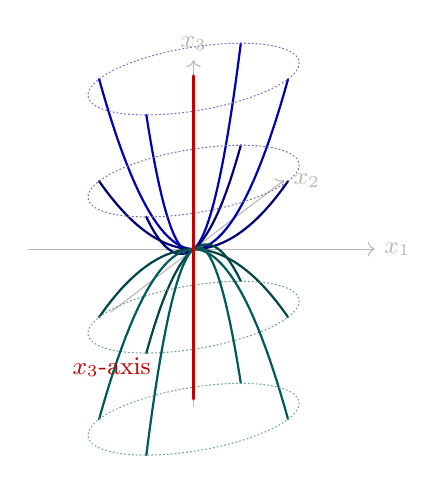
\begin{tikzpicture}[x={(1cm,0cm)}, y={(0.50cm,0.38cm)}, z={(0cm,1cm)}, line cap=round]
  \draw[->,gray!55] (-2.1,0,0)--(2.3,0,0) node[right]{\small$x_1$};
  \draw[->,gray!55] (0,-2.1,0)--(0,2.3,0) node[right]{\small$x_2$};
  \draw[->,gray!55] (0,0,-2.0)--(0,0,2.4) node[above]{\small$x_3$};
  \foreach \r/\col in {1.5/blue!70!black, 0.6/blue!45!black, -0.6/teal!55!black, -1.5/teal!70!black}{
    \draw[\col,thick,domain=-1.2:1.2,samples=50,variable=\t] plot ({\t},{0},{\r*\t*\t});
    \draw[\col,thick,domain=-1.2:1.2,samples=50,variable=\t] plot ({0},{\t},{\r*\t*\t});
    \draw[\col!55,densely dotted,domain=0:360,samples=60,variable=\a]
         plot ({1.2*cos(\a)},{1.2*sin(\a)},{\r*1.44});
  }
  \draw[very thick,red!75!black] (0,0,-1.9)--(0,0,2.2);
  \node[red!75!black,left] at (-0.42,0,-1.5) {\small$x_3$-axis};
\end{tikzpicture}}\\[2pt]\small(a)
\end{minipage}\hfill
\begin{minipage}[b]{0.48\textwidth}\centering
\scalebox{0.85}{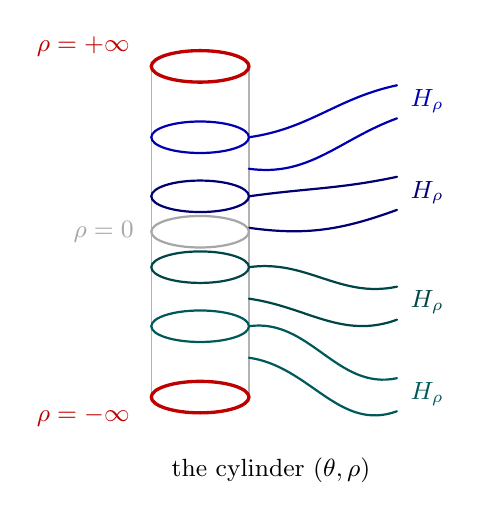
\begin{tikzpicture}[line cap=round]
  \def\rx{0.62}\def\ry{0.20}
  \draw[gray!60] (-\rx,-2.1) -- (-\rx,2.1);
  \draw[gray!60] ( \rx,-2.1) -- ( \rx,2.1);
  \draw[red!75!black,very thick] (0,2.1) ellipse ({\rx} and {\ry});
  \draw[red!75!black,very thick] (0,-2.1) ellipse ({\rx} and {\ry});
  \node[red!75!black,left] at (-\rx-0.15,2.35) {\small$\rho=+\infty$};
  \node[red!75!black,left] at (-\rx-0.15,-2.35) {\small$\rho=-\infty$};
  \foreach \h/\col in {1.2/blue!70!black, 0.45/blue!45!black, -0.45/teal!55!black, -1.2/teal!70!black}{
    \draw[\col,thick] (0,\h) ellipse ({\rx} and {\ry});
    \draw[\col,thick] (\rx,\h) to[out=8,in=192] (2.5,\h+0.55*\h);
    \draw[\col,thick] (\rx,\h-2*\ry) to[out=-8,in=200] (2.5,\h+0.55*\h-0.42);
    \node[\col,right] at (2.55,\h+0.55*\h-0.2) {\small$H_{\rho}$};
  }
  \draw[gray!70,thick] (0,0) ellipse ({\rx} and {\ry});
  \node[gray!70,left] at (-\rx-0.1,0) {\small$\rho=0$};
  \node[below] at (0.9,-2.75) {\small the cylinder $(\theta,\rho)$};
\end{tikzpicture}}\\[2pt]\small(b)
\end{minipage}
\caption{(a) The horns $H_\rho=\{x_3=\rho r^{2}\}$ in $x$-space: paraboloids of revolution
with a common apex at the origin, tangent there to the plane $x_3=0$. They foliate
$\R^{3}$ minus the $x_3$-axis (thick), which is their common limit as
$\rho\to\pm\infty$. (b) After the blow-up: in the formula \eqref{eq:chart1} the set $\{r=0\}$
is the cylinder with coordinates $(\theta,\rho)$, and the whole cylinder maps to the original origin; each
horn is attached along one circle $\rho=\mathrm{const}$ (the circle $\rho=0$ along the plane $x_3=0$). The two end
circles $\rho=\pm\infty$ are not part of the cylinder. The circles over the points $(0,0,x_3)$ of the $x_3$-axis lie in
the chart \eqref{eq:chart2}, not on the cylinder; as $x_3\to0^{\pm}$ they approach the ends $\rho=\pm\infty$. The synthesis of \S\ref{sec:entry} below drives $\rho$ from the two
ends towards the circle $\rho=0$.}\label{fig:horns}
\end{figure}

\emph{Area is the only way to move $x_3$.} Writing $x_1=r\cos\theta$, $x_2=r\sin\theta$,
a control is the velocity of that point, and
\begin{equation}\label{eq:swept}
  \dot x_3=x_1u_2-x_2u_1=r^{2}\,\dot\theta .
\end{equation}
The right-hand side is twice the areal velocity of the projected motion:
$x_1\dot x_2-x_2\dot x_1=r^{2}\dot\theta$.
\subsection{The synthesis: outward motion, then descent}\label{sec:entry}
The construction has two regimes, and the horn label $\rho$ decides between them: where
$|\rho|$ is large the state runs outward at constant height (the \emph{outward motion}), which is what brings $|\rho|$
down, and where $|\rho|$ is small it descends (the \emph{descent}) to the working point with the radius and the height
decaying at rates of their own.

\emph{The plant on the blow-up.} In the coordinates $(\nu,\theta,\rho)$ of the first chart
\eqref{eq:chart1}, with $\nu=r(1+\rho^{2})^{1/4}$, write the control as
\begin{equation}\label{eq:ABframe}
  u=\nu A\,e_r+\nu(1+\rho^{2})^{1/4}B\,e_\theta,\qquad
  e_r=(\cos\theta,\sin\theta),\quad e_\theta=(-\sin\theta,\cos\theta),
\end{equation}
so that $\dot r=\nu A$ and $\dot x_3=\nu^{2}B$. The new controls are $A,B\in\R$. The plant
\eqref{eq:brockett} lifted to the blow-up is
\begin{align}
  \dot\rho&=B\,(1+\rho^{2})^{1/2}-2\rho A\,(1+\rho^{2})^{1/4}, \label{eq:shape-AB}\\
  \frac{\dot\nu}{\nu}&=A\,(1+\rho^{2})^{-3/4}+\tfrac12\,\rho B\,(1+\rho^{2})^{-1/2},
    \label{eq:size-AB}\\
  \dot\theta&=B\,(1+\rho^{2})^{1/2},\notag
\end{align}
and the size of the control is
\begin{equation}\label{eq:cost-AB}
  |u|^{2}=\nu^{2}\bigl[A^{2}+B^{2}(1+\rho^{2})^{1/2}\bigr].
\end{equation}
The right-hand sides do not contain $\nu$ or $\theta$, so the lifted system extends to the
cylinder $\nu=0$ over the origin, which is invariant.

\emph{The control bound.} We require $|u|\le c\,\nu$ with a constant $c>0$. By \eqref{eq:cost-AB} it reads
\begin{equation}\label{eq:bound-AB}
  A^{2}+B^{2}(1+\rho^{2})^{1/2}\le c^{2}.
\end{equation}
This bound decides how far from the axis the state must go before it can descend.
Near the axis, moving outward is cheap and moving the height is expensive, so the state first moves
away from the axis and only then descends (Appendix~\ref{app:brockett}).

\emph{The reference.} Let $Z$ denote the blow-up of \S\ref{sec:horns} above, in the two
formulas \eqref{eq:chart1} and \eqref{eq:chart2}, and let $\beta\colon Z\to\R^{3}$ be the
blow-down. Here the reference, the coupling $h$ and the map $F=\beta$ are defined globally, on all of $Z$,
not only near one point as in the Definition of \S\ref{sec:product}. The reference $\dot z$ on $Z$ is as follows, with constants
$b>2a>0$, $\eta>0$ and $\rho_0>0$ chosen by the designer.

\emph{Outward motion}, on $|\rho|>\rho_0$, in the coordinates $(r,\theta,x_3)$ of \eqref{eq:chart2}:
\begin{equation}\label{eq:entry}
  \dot r=\eta\,\nu,\qquad \dot\theta=0,\qquad \dot x_3=0,
\end{equation}
with $\nu=(r^{4}+x_3^{2})^{1/4}$. In the coordinates $(\nu,\theta,\rho)$ it reads
$\dot\rho=-2\eta\rho(1+\rho^{2})^{1/4}$, $\dot\theta=0$, $\dot\nu/\nu=\eta(1+\rho^{2})^{-3/4}$, which
also covers the cylinder $\nu=0$.

\emph{Descent}, on $|\rho|\le\rho_0$, in the coordinates $(\nu,\theta,\rho)$ of \eqref{eq:chart1}:
\begin{equation}\label{eq:tworates}
  \dot\rho=-(b-2a)\rho,\qquad \dot\theta=-b\rho,\qquad
  \frac{\dot\nu}{\nu}=-\,\frac{a+\frac12 b\rho^{2}}{1+\rho^{2}}.
\end{equation}

\emph{The coupling} $u=h(z)$ is
\begin{equation}\label{eq:coupling}
  u=\eta\,\nu\,e_r\quad\text{on }\{|\rho|>\rho_0\},\qquad
  u=-r\,(a\,e_r+b\rho\,e_\theta)\quad\text{on }\{|\rho|\le\rho_0\},
\end{equation}
with $r=\nu(1+\rho^{2})^{-1/4}$. It is the control \eqref{eq:ABframe} with $A=\eta$, $B=0$ in the
outward motion and $A=-a(1+\rho^{2})^{-1/4}$, $B=-b\rho(1+\rho^{2})^{-1/2}$ in the descent, and under it the
lifted plant \eqref{eq:shape-AB}--\eqref{eq:size-AB} is the reference. Pushed down by
$\beta$ it gives the feedback in $x$. Write $r=(x_1^{2}+x_2^{2})^{1/2}$, $\nu(x)=(r^{4}+x_3^{2})^{1/4}$
and $\rho(x)=x_3/r^{2}$. Then
\begin{equation}\label{eq:feedback}
  u=\begin{cases}
    \eta\,\nu(x)\,\dfrac{(x_1,x_2)}{r}
      & \text{where } |x_3|>\rho_0\,r^{2}\quad\text{(outward motion)},\\[2ex]
    -a\,(x_1,x_2)-b\,\rho(x)\,(-x_2,x_1)
      & \text{where } |x_3|\le\rho_0\,r^{2}\quad\text{(descent)},
  \end{cases}
\end{equation}
and $u(0)=0$. The two regions are separated by the horns $|x_3|=\rho_0r^{2}$.

The checks that both formulas are bounded, that the switch is crossed once, and the largest admissible
$\rho_0$ are given in Appendix~\ref{app:brockett}.

\emph{The coupling manifold is the graph of the blow-down.} It is
\[
  M=\graph\bigl(x=\beta(z)\bigr)\subset X\times Z,
\]
invariant under the product system because the closed loop is by construction the
push-forward of the reference. Here $\beta$ is a local diffeomorphism off the exceptional
set $E$, so
\[
  \Sig=E,\qquad \pi(\Sig)=\{\,x_1=x_2=0\,\},
\]
the ramification locus is the $x_3$-axis. The fibre of $\pi$ over a point of the axis other than
the origin is the fibre of $\beta$, a circle; over the origin it is the cylinder $\{r=0\}$ of
\eqref{eq:chart1}. So $\beta$ fails to be a diffeomorphism exactly on $E$.

\begin{proposition}[the branching feedback]
Let $a,b,\eta,\rho_0>0$ with $b>2a$, and write $r=(x_1^{2}+x_2^{2})^{1/2}$,
$\nu(x)=(r^{4}+x_3^{2})^{1/4}$, $\rho(x)=x_3/r^{2}$. The branching feedback of the coupling
\eqref{eq:coupling} is
\begin{equation}\label{eq:branchfb}
  u(x,\theta)=\begin{cases}
    \eta\,\nu(x)\,(x_1,x_2)/r & \text{if } r>0,\ |x_3|>\rho_0r^{2},\\[0.5ex]
    \eta\,|x_3|^{1/2}(\cos\theta,\sin\theta) & \text{if } r=0,\ x_3\neq0,\\[0.5ex]
    -a\,(x_1,x_2)-b\,\rho(x)\,(-x_2,x_1) & \text{if } r>0,\ |x_3|\le\rho_0r^{2},\\[0.5ex]
    0 & \text{if } x=0,
  \end{cases}
\end{equation}
where the branch $\theta\in S^{1}$ is the point of the circle $\beta^{-1}(x)$ over an axis point; off the axis
there is one branch and $u$ does not depend on $\theta$. Thus $u(x,\theta)=h(z)$, with $z$ the point of
$\beta^{-1}(x)$ of angle $\theta$, and $u$ is the coupling on $Z$; it extends continuously to the axis within the outward-motion region and is
continuous within each regime.
\begin{enumerate}
\item[\textup{(i)}] For every initial state $x(0)$ and branch $\theta(0)$ the closed loop has a unique
      lifted solution, $x(t)=\beta(z(t))$, where $z(t)$ is the solution of the reference from the point of
      $\beta^{-1}(x(0))$ of angle $\theta(0)$. The branch matters only if $x(0)$ is on the axis.
\item[\textup{(ii)}] A solution that starts on the axis leaves it at once in the direction $\theta(0)$, and no
      solution reaches the axis at a later time. So the branch is chosen once, at $t=0$, and never switched.
\end{enumerate}
\end{proposition}

\emph{The choice of branch.} Every branch gives the same motion of $r$ and $x_3$, the same times and the
same estimates; the branch fixes only the direction in which the state leaves the axis. One may also fix
one branch $\theta_0$ for all axis points; this gives a feedback $u(x)=u(x,\theta_0)$ without a branch
argument, with the same estimates. Uniqueness in (i) refers to the closed loop with its branch, that is, to
solutions with a continuous lift to $Z$. For the static $u(x)$, a solution starting on the axis may leave it in
any direction, with the same estimates. By Brockett's condition \cite{Brockett1983} no continuous $u(x)$
stabilises the origin, and indeed $u(x)$ is discontinuous at every point $x^{*}=(0,0,x_3)$, $x_3\neq0$, of the
$x_3$-axis: $u(x^{*})=\eta|x_3|^{1/2}(\cos\theta_0,\sin\theta_0)$, while at the points
$x=(-\varepsilon\cos\theta_0,-\varepsilon\sin\theta_0,x_3)$, which tend to $x^{*}$ as $\varepsilon\to0$, $u(x)$ tends
to $-u(x^{*})$. The discontinuity at the axis is not seen along any solution.

\begin{proposition}[the estimates]
In the setting of the previous Proposition, let $x(t)$ be a solution of the
closed loop with the branching feedback \eqref{eq:branchfb}, with $x(0)\neq0$ and any branch $\theta(0)$,
and write $u(t)=u(x(t),\theta(0))$. Put
\[
  C=(1+\rho_0^{-2})^{1/4},\qquad
  c=\max\Bigl\{\eta,\ \max_{|\rho|\le\rho_0}\sqrt{a^{2}+b^{2}\rho^{2}}\,(1+\rho^{2})^{-1/4}\Bigr\}.
\]
Then:
\begin{enumerate}
\item[\textup{(i)}] $|u(t)|\le c\,\nu(x(t))\le cC\,\nu(x(0))$ --- the control is bounded by
      the size $\nu$, hence bounded on each neighbourhood of the origin and vanishing
      at it;
\item[\textup{(ii)}] the region $\{|\rho|\le\rho_0\}$ is reached by the time
      \begin{equation}\label{eq:entrytime}
        T_{\mathrm{out}}=\frac{\tau(\rho_0)}{\eta},\qquad
        \tau(\rho_0)=\int_0^{\rho_0^{-1/2}}\frac{d\xi}{(1+\xi^{4})^{1/4}} ,
      \end{equation}
      which does not depend on $x(0)$, and is not left again;
\item[\textup{(iii)}] afterwards $\rho(t)\to0$ exponentially at rate $b-2a$, and
      \eqref{eq:tworates} gives
      \[
        \nu(x(t))\le C\,\nu(x(0))\,e^{-a(t-T_{\mathrm{out}})};
      \]
\item[\textup{(iv)}] consequently the attraction is uniform: given
      $\varepsilon>0$, one has
      $\nu(x(t))\le\varepsilon\,\nu(x(0))$ for all
      $t\ge T(\varepsilon)=\tau(\rho_0)/\eta+a^{-1}\log(C/\varepsilon)$, with
      $T(\varepsilon)$ independent of the initial point; in particular the
      \emph{half-attraction time} $T(1/2)=\tau(\rho_0)/\eta+a^{-1}\log(2C)$, after which
      $\nu(x(t))\le\frac12\,\nu(x(0))$, is the same for every initial point, and each
      further halving takes at most $T(1/2)$;
\item[\textup{(v)}] the path length $\int_0^\infty|u|\,dt$ and the energy
      $\int_0^\infty|u|^{2}\,dt$ are at most constant multiples of $\nu(x(0))$ and
      $\nu(x(0))^{2}$.
\end{enumerate}
\end{proposition}

The horns have played no part in this beyond labelling the two regimes; they are
crossed, not preserved. What preserving them would give instead is recorded in
\S\ref{sec:leaf} below.


The switching surface $|\rho|=\rho_0$ can be removed (Appendix~\ref{app:brockett}).

\subsection{The horns as invariant leaves}\label{sec:leaf}
The synthesis of \S\ref{sec:entry} above crosses the horns. Here they are kept invariant instead, as the
blow-up suggests: one reference for each horn. This gives two things the synthesis of \S\ref{sec:entry}
does not have, a rotation at a prescribed frequency and the clock used in \S\ref{sec:rotating} below.

A reference preserves every horn exactly when $\dot\rho=0$, that is by \eqref{eq:shape-AB} when
$B=2\rho A(1+\rho^{2})^{-1/4}$. Write $\dot r=-\frac12k\,r$ and $\dot x_3=-k\,x_3$, which is this condition
with $k=-2A(1+\rho^{2})^{1/4}$. On the horn labelled $\rho$ the state then turns and shrinks at the rates
\begin{equation}\label{eq:leafclock}
  \omega=\dot\theta=-k\rho,\qquad \frac{\dot\nu}{\nu}=-\frac k2,\qquad |u|=k\,r\sqrt{\tfrac14+\rho^{2}} .
\end{equation}
Since $\rho$ is constant along the motion, $k$ may be any positive function of $\rho$; the fastest one
allowed by $|u|\le c\nu$ is
\begin{equation}\label{eq:kopt}
  k(\rho)=\frac{2c\,(1+\rho^{2})^{1/4}}{\sqrt{1+4\rho^{2}}},\qquad
  k(\rho)\sim\frac{c}{|\rho|^{1/2}}\ \ (\rho\to\pm\infty).
\end{equation}
The horns alone do not give uniform attraction: the rate $k/2$ tends to $0$ near the axis, and no other
choice of $k$ helps, because $|\dot x_3|=|x_1u_2-x_2u_1|\le r|u|$ while on an invariant horn the radius $r$
only decreases, so lowering the height of a state close to the axis takes a long time.

\emph{The outward motion or a rotation, then a horn.} If $|\rho(0)|>\rho_0$, run the outward motion
\eqref{eq:entry} until $|\rho|=\rho_0$; it lasts at most $\tau(\rho_0)/\eta$. If $|\rho(0)|<\rho_0$, rotate the
state about the $x_3$-axis instead, with $u=\sigma c\nu\,e_\theta$, $\sigma=\operatorname{sign}x_3(0)$ (either sign if
$x_3(0)=0$: two branches). Then $r$ is constant, $\dot x_3=\sigma c\nu r$ and
$\frac{d}{dt}|\rho|=c(1+\rho^{2})^{1/4}\ge c$, so $|\rho|=\rho_0$ is reached within the time $\rho_0/c$, and $\nu$
grows at most by the factor $(1+\rho_0^{2})^{1/4}$. At the first arrival at $|\rho|=\rho_0$ switch to the horn-preserving law: keep the state on the horn it has
reached, with
the rate \eqref{eq:kopt}, so $k=k(\rho_0)$ and the attraction is uniform:
\[
  \nu\bigl(x(t)\bigr)\le C\,\nu\bigl(x(0)\bigr)\,e^{-\frac12k(\rho_0)\,(t-T_0)},
\]
with
\[
  C=\max\bigl\{(1+\rho_0^{-2})^{1/4},(1+\rho_0^{2})^{1/4}\bigr\},\quad
  T_0=\max\bigl\{\tau(\rho_0)/\eta,\ \rho_0/c\bigr\}.
\]
\emph{The law as a function of the state, the branch and a mode.} Put $e_r=(x_1,x_2)/r$,
$e_\theta=(-x_2,x_1)/r$, $\rho(x)=x_3/r^{2}$, $k=k(\rho_0)$ and, with a constant $\gamma>0$,
$q(x)=\rho(x)+(\gamma/k)\bigl(\rho(x)-\sigma\rho_0\bigr)$. The closed loop carries, besides the branch, a
mode $m\in\{0,1\}$, which is switched by the switching rule $\beta_{\mathrm{sw}}$: from the present state
$x(t)$ and the mode $m(t-0)$ just before the present moment, it gives the mode $m(t+0)$ just after it,
\[
  m(t+0)=\beta_{\mathrm{sw}}\bigl(x(t),m(t-0)\bigr),\qquad \beta_{\mathrm{sw}}(x,1)=1,\qquad
  \beta_{\mathrm{sw}}(x,0)=\begin{cases}1&\text{if } r>0,\ |x_3|=\rho_0r^{2},\\ 0&\text{otherwise},\end{cases}
\]
and $m(t_0)=\beta_{\mathrm{sw}}\bigl(x(t_0),0\bigr)$: $m$ becomes $1$ when the state first reaches $|\rho|=\rho_0$, which a
continuous trajectory cannot jump over, and never returns to $0$. The law is
\[
  u(x,\theta,\sigma,m)=\begin{cases}
    \eta\,\nu\,e_r & \text{if } m=0,\ r>0,\ |x_3|>\rho_0r^{2},\\[0.5ex]
    \eta\,|x_3|^{1/2}(\cos\theta,\sin\theta) & \text{if } m=0,\ r=0,\ x_3\neq0,\\[0.5ex]
    \sigma c\,\nu\,e_\theta & \text{if } m=0,\ r>0,\ |x_3|<\rho_0r^{2},\\[0.5ex]
    -k\bigl(\tfrac12(x_1,x_2)+q(x)\,(-x_2,x_1)\bigr) & \text{if } m=1,\\[0.5ex]
    0 & \text{if } x=0,
  \end{cases}
\]
where the branch $\theta\in S^{1}$ is used over an axis point and $\sigma=\operatorname{sign}x_3$, with the two
branches $\sigma=\pm1$ if $x_3=0$. Both are chosen at $t_0$ and never switched, $\theta(t+0)=\theta(t-0)$,
$\sigma(t+0)=\sigma(t-0)$: a trajectory starting on the axis leaves it at once and does not return, and $x_3\neq0$
with the sign $\sigma$ for $t>t_0$. So $m$ is the only switch. The horn law cannot be used on the surface
$|x_3|=\rho_0r^{2}$ alone. The outward motion and the rotation both push the state onto this surface from its two
sides. An exact solution could follow the horn law on the surface, but with any error in measuring the state or
in the switching, and for solutions in Filippov's sense, a law depending on $x$ alone would alternate between
the two near the surface (jitter), and the state would slide along the surface under a combination of the two motions. Both increase $\nu$, since
$\frac{d}{dt}\nu^{4}=4r^{3}\dot r+2x_3\dot x_3$ is positive for each of them, so the sliding state moves away from
the origin. The mode prevents this. It is not necessary for that: since the law for
$m=1$ makes the horn $\rho=\sigma\rho_0$ attracting (see below), it could be used without a mode on a layer
$\rho_0-\delta\le|\rho|\le\rho_0+\delta$, whose edges the laws on both sides cross only inwards; with errors of size $E$ in the measured $\rho$ this
needs $\gamma\delta>(k+\gamma)E$. The mode is
nevertheless beneficial: the law changes only once, at the first arrival, and after that a disturbance never
returns the state to the outward motion or the rotation. With errors in measuring the state, the switch takes
place when the measured state first reaches or crosses the horn, and this ends the approach. Later crossings of
the horn caused by errors do not change the law: the law for $m=1$ is the same on both sides of the horn,
depends continuously on $x$ there and pulls the state back towards the horn, so the state only wobbles around
it. Without the mode, on a layer, errors near its edges could switch the law back and forth during the entry. The mode, like the branch, is a part of the state of the closed loop and is constant between
switches (\S\ref{sec:core}); with it there is no jitter, since after the switch the law for $m=1$ is the only one
in use and the switching law no longer depends on $x$.

For $m=1$ one has $\dot r=-\frac12k\,r$ and $\dot\rho=-\gamma(\rho-\sigma\rho_0)$. Without errors the state stays
on the horn $\rho=\sigma\rho_0$, where $q=\rho$, and moves there as in \eqref{eq:leafclock} with $k=k(\rho_0)$. The
term with $\gamma$ makes this horn attracting. Let $\rho$ be measured with an error $e(t)$,
$|e|\le E$; this is an error model for $\rho$ itself, since bounded errors in $x_3$ and $r$ need not give bounded
errors in $x_3/r^{2}$ as $r\to0$. Without the term ($\gamma=0$) every horn is kept and none is preferred:
$\dot\rho=-k\,e$, and the errors can accumulate. With $\gamma>0$, $h=\rho-\sigma\rho_0$ obeys
$\dot h=-\gamma h-(k+\gamma)e$, so, with $t$ counted from the switch,
\[
  |h(t)|\le e^{-\gamma t}|h(0)|+\frac{k+\gamma}{\gamma}\,E\,\bigl(1-e^{-\gamma t}\bigr):
\]
$\rho$ stays in a band around $\sigma\rho_0$ of width of the order of $E$ that does not grow with time, and the
angular velocity $k|q|$ stays correspondingly close to $|\omega_*|$ below. Without errors
$|u|\le\max\{\eta,c\}\,\nu$ along the whole motion, with $|u|=c\nu$ on the target horn; with errors the constant
for $m=1$ is enlarged according to the band.

Every trajectory ends on a horn $|\rho|=\rho_0$ and spirals into the origin with the constant angular
velocity
\begin{equation}\label{eq:freq}
  |\omega_*|=k(\rho_0)\rho_0=\frac{2c\,\rho_0\,(1+\rho_0^{2})^{1/4}}{\sqrt{1+4\rho_0^{2}}},
\end{equation}
which increases from $0$ to $\infty$ with $\rho_0$: every frequency is available, and the designer chooses
it through $\rho_0$. In \S\ref{sec:entry}, by contrast, $\rho\to0$ and the rotation dies out. The result is a
decaying spiral of prescribed frequency; \S\ref{sec:frequency} below obtains a periodic motion of
prescribed frequency by the same mechanism.

\subsection{A continuous time-periodic law from a rotating branch}\label{sec:rotating}
The branching feedback \eqref{eq:branchfb} has a circle of branches over the axis. A continuous feedback
that does not depend on time cannot stabilise the plant, by Brockett's condition \cite{Brockett1983}; a
time-dependent one is not subject to that condition. Here the branch used on the axis is made to rotate, in opposite directions on
the upper and the lower half-axis, and inside a thin tube around the axis the branches are merged into one
value. The result
is a continuous time-periodic stabiliser. Outside the tube it is the smooth field \eqref{eq:smoothAB}, so
\S\ref{sec:entry}--\S\ref{sec:leaf} above supply most of the proof; only the analysis near the axis is new.

\emph{The sphere of shapes.} The dilations $\delta_\lambda(x_1,x_2,x_3)=(\lambda x_1,\lambda x_2,\lambda^{2}x_3)$,
$\lambda>0$, carry each state $x\neq0$ to exactly one point of the surface $S=\{\nu=1\}$, its \emph{shape}. The
surface $S$ is a sphere with the poles $(0,0,\pm1)$ on the axis and the equator in the plane $x_3=0$. The laws
of this section are homogeneous, $u(\delta_\lambda x)=\lambda u(x)$, so the closed loop commutes with the
dilations and moves the shapes along a vector field on $S$, the \emph{shape field}. At a zero of the shape
field off the equator a state keeps $\theta$ and $\rho$; since $\dot x_3=r^{2}\dot\theta$, it then keeps $x_3$ and
$r$, so it does not move. Take a continuous static law that equals \eqref{eq:smoothAB} away from the axis. Its
shape field is continuous on a cap $\{\rho\ge\rho_c\}$ around the north pole and, by $\dot\rho<0$ for
\eqref{eq:smoothAB}, points out of the cap on its boundary circle. A vector field on a closed disk that points
outward on the boundary vanishes inside, so the law has a state that does not move, as Brockett's condition
requires. The blow-up replaces each pole by the circle of branches and turns $S$ into a cylinder; on the
cylinder the shape field of \eqref{eq:smoothAB} vanishes only on the equator, where the states shrink in the
plane $x_3=0$. This is why the branching feedback has no state that does not move. The law below is
continuous, so the zero in the cap is there again, but now as a zero of the shape field in the frame that
rotates with the branch: a state there keeps its shape and turns with the branch, $\dot\theta=\omega$, and
\eqref{eq:leafclock} gives $\dot\nu/\nu=\omega/(2\rho)$. Turning against the sign of $x_3$ makes it shrink. The
chart $y$ in the proof (Appendix~\ref{app:rotating} below) is the chart of $S$ at the north pole in the rotating
frame; step (b) of the proof gives the boundary circle of the cap, step (c) treats the zeros inside it, and the
Remark after the Theorem below is the case of the wrong direction of rotation.

\emph{The law.} Let $A(\rho)$, $B(\rho)$ be the pair \eqref{eq:smoothAB}, with $\eta,a>0$ and $b>2a$. Put
$w=r/\nu=(1+\rho^{2})^{-1/4}\in[0,1]$, so that $w=0$ on the axis and $w=1$ on the plane $x_3=0$. Fix a tube
width $w_1\in(0,1)$, a frequency $\omega_0>0$ and a phase $\varphi_0$, and let
\[
  \sigma(w)=3(w/w_1)^{2}-2(w/w_1)^{3}\ (w\le w_1),\qquad \sigma(w)=1\ (w\ge w_1),
\]
\[
  e_\pm(t)=\bigl(\cos(\mp\omega_0t+\varphi_0),\,\sin(\mp\omega_0t+\varphi_0)\bigr).
\]
The \emph{tube} is $\{w<w_1\}$. Define $u(0,t)=0$ and, for $x\neq0$,
\begin{equation}\label{eq:rotlaw}
  u(x,t)=\nu A(\rho)\Bigl[\sigma(w)\frac{(x_1,x_2)}{r}+\bigl(1-\sigma(w)\bigr)e_{\operatorname{sgn}x_3}(t)\Bigr]
  +\nu(1+\rho^{2})^{1/4}B(\rho)\,\frac{(-x_2,x_1)}{r}.
\end{equation}
Outside the tube $\sigma=1$ and \eqref{eq:rotlaw} is the smooth field \eqref{eq:smoothAB}. On the axis it is
$u=\eta\nu\,e_\pm(t)$: the branch of \eqref{eq:branchfb} used at time $t$ is $\theta=\mp\omega_0t+\varphi_0$,
which rotates with period $P=2\pi/\omega_0$. The law is continuous: $e_\pm$ enters only inside the tube,
where $x_3\neq0$ keeps its sign; near the axis
$\sigma(w)(x_1,x_2)/r=3w_1^{-2}r(x_1,x_2)/\nu^{2}-2w_1^{-3}r^{2}(x_1,x_2)/\nu^{3}$ tends to $0$; and the last term
equals $-b\,x_3r^{2}(-x_2,x_1)/\nu^{4}$. It is $C^{1}$ in $x\neq0$, satisfies $|u|\le(\eta+a+b)\nu$, and is
homogeneous: $u(\lambda x_1,\lambda x_2,\lambda^{2}x_3,t)=\lambda u(x,t)$.

\begin{theorem}[continuous stabilisation by a rotating branch]
For all $\eta,a>0$, $b>2a$, $w_1\in(0,1)$ and $\omega_0>0$, the closed loop \eqref{eq:brockett},
\eqref{eq:rotlaw} has unique solutions defined for all $t\ge t_0$, and there are $K,\gamma>0$, independent of
$t_0$ and $x(t_0)$, such that $\nu(x(t))\le Ke^{-\gamma(t-t_0)}\nu(x(t_0))$ for $t\ge t_0$.
\end{theorem}

The proof is in Appendix~\ref{app:rotating} below.

\begin{remark}[the opposite rotation is necessary]
If both half-axes rotate the same way, $\varphi(t)=\omega t+\varphi_0$, the circle of step (b) of the proof in Appendix~\ref{app:rotating} is unchanged, since
$\ell$ does not involve $\omega$. The field has index one on it, so it has an equilibrium inside, and there
$\dot\nu/\nu=\omega/(2\rho)$. In the half-space where $\omega x_3>0$ this is positive: the corresponding solution
grows exponentially, and by the dilations such solutions start arbitrarily close to the origin, which is
therefore neither stable nor attractive. The sign rule ``rotate against the sign of $\rho$'' is the clock
$\omega=-k\rho$ of \eqref{eq:leafclock}.
\end{remark}
For a frozen time the law \eqref{eq:rotlaw} is a continuous selection of the branching feedback away from the
axis, smoothed across it; the time dependence serves only to move the selected branch around the circle of
branches. With $\omega_0=0$ the smoothed law is static and continuous, and it acquires the spurious equilibria
that Brockett's condition predicts.


\section{Control of frequency}\label{sec:frequency}
% =====================================================================

We consider the plant \eqref{eq:plant} at a working point where the linearisation $(A,C)$ is
uncontrollable, with a critical oscillatory pair $\pm i\omega_0$ ($\omega_0\ge0$) among the
uncontrollable modes. Smooth feedback leaves the uncontrollable eigenvalues $\pm i\omega_0$ in the
spectrum of the closed-loop linearisation, so a Hopf cycle born from that pair under smooth
feedback has onset frequency $\omega_0$. The \emph{control-of-frequency} problem is to install by
feedback an attracting cycle on which $x_<$ moves at a prescribed
angular velocity. Three frequencies must be kept apart. The reference cycle has angular frequency
$\omega$. The coupling manifold is $x_<=z^{2}$, so $x_<=z^{2}$ moves at
angular velocity $2\omega$ (at $-2\omega$ for $x_<=\bar z^{2}$). The whole closed-loop orbit, control
included, has period $2\pi/\omega$. The Theorem of \S\ref{sec:general-freq} below assigns the angular
velocity $\pm2\omega$ of $x_<$, for every $\omega>0$ except $2\omega=\omega_0$ in
the rotation $+2$, when the quadratic part $Q$ of the control has no folds.
\S\ref{sec:reachable} below records what a \emph{linear} coupling gives at second order, and the Theorems of \S\ref{sec:friction} and \S\ref{sec:friction-full} below show that a
linear coupling with a cubic friction term realises every frequency that passes that test, whether or not $Q$ has
folds, for the plane system and for the full plant, up to a few resonances.

\subsection{The construction}\label{sec:critical-pair}
Consider the plant \eqref{eq:plant} at a working point $x=0$, $u=0$ where the linearisation
$(A,C)$ is uncontrollable at a critical oscillatory pair $\pm i\omega_0$ ($\omega_0\ge0$). The
Kalman decomposition of $(A,C)$ splits the state, $x=(x_<,x_>)$, into the uncontrollable
linearly uncontrollable part $x_<\in\C\cong\R^{2}$, carrying that pair, and a controllable complement $x_>$,
bringing \eqref{eq:plant} to the normal form
\begin{equation}\label{eq:split}
  \dot x_<=i\omega_0 x_<+Q(u,x),\qquad \dot x_>=A_> x_>+A_{><}x_<+C_> u+R(u,x),
\end{equation}
in which $u\in\R^{\ell}$ is the \emph{full} control, and $Q(u,x)$, $R(u,x)$ collect the terms of
order $\ge2$ in the two equations --- $Q$ two-dimensional, valued in the critical plane. (The
Kalman form allows the linear coupling $A_{><}x_<$ in the controllable block; the critical block
receives nothing linear.) The
linearly uncontrollable part $x_<$ turns at $\pm i\omega_0$ under \emph{no} linear control --- so the control
reaches the critical mode only through $Q$ --- while $(A_>,C_>)$ is controllable. We
assume
\begin{itemize}
\item[(H1)] the uncontrollable subspace is two-dimensional with critical pair $\pm i\omega_0$
  (for $\omega_0=0$ the uncontrollable block is assumed to be $0$), and the quadratic-in-$u$ part of $Q$ not identically zero;
\item[(H2)] the complement $(A_>,C_>)$ is controllable, and $\dim_{\R}\ker C_>=2$.
\end{itemize}

\begin{remark}[the dimensions here need not be minimal]
Both dimensions above are fixed at their smallest values, not their only possible ones. The
uncontrollable subspace of (H1) is taken to be exactly two-dimensional, carrying just the pair
$\pm i\omega_0$; it could instead be higher-dimensional, with $\pm i\omega_0$ appearing as one
invariant block among others. Likewise $\dim_{\R}\ker C_>$ in (H2) is fixed at $2$; it could
instead exceed $2$. Neither possibility is pursued here.
\end{remark}

Assume $x_>=0$ and let $u$ range over $\ker C_>$, identified with $\C$ by (H2) --- chosen so as
not to disturb the complement once it is switched back on in \S\ref{sec:general-freq} --- in the
first equation
$\dot x_<=i\omega_0 x_<+Q(u,x)$ of \eqref{eq:split}; such $u$ leaves the complement equation
untouched, since $C_>u=0$. Redefine $x_<$ as $x$. Then
$Q$, in the control alone, is the general $\C$-valued real quadratic
\[
  Q(u)=G\,u^{2}+H\,|u|^{2}+K\,\bar u^{2}\qquad(G,H,K\in\C).
\]
The terms $u\cdot x$, $x^{2}$ and those of order three are of higher order in the reference
variable below ($u\sim z$, $x\sim z^{2}$), and the \emph{plane system} is
\begin{equation}\label{eq:model-w0}
  \dot x=i\omega_0 x+Q(u),\qquad x,u\in\C,
\end{equation}
uncontrollable at its linearisation ($\partial_uQ|_0=0$). For $\omega_0=0$ and $Q(u)=u^{2}$ it is
the model \eqref{eq:model} with $n=2$; for $\omega_0=0$ and other $Q$ it need not resemble that
model (for $Q(u)=|u|^{2}$, $\operatorname{Re}x$ never decreases and $\operatorname{Im}x$ is constant).
The full plant is taken up again in \S\ref{sec:general-freq}.

Fix $\omega>0$ and take for reference the Andronov--Hopf system
\begin{equation}\label{eq:hopf-ref}
  \dot z=w(z):=(\varepsilon+i\omega)z-|z|^{2}z,\qquad z\in\C\cong\R^{2},\quad\varepsilon>0,
\end{equation}
whose attracting cycle $|z|^{2}=\varepsilon$ carries $\dot z=i\omega z$. The first coupling to try is
the real-linear $p(z)=bz+b'\bar z$. With
$Q(p(z))=d_{20}z^{2}+d_{11}z\bar z+d_{02}\bar z^{2}$,
\begin{equation}\label{eq:drive}
  d_{20}=Gb^{2}+Hb\bar b'+K\bar b'^{2},\quad
  d_{11}=2Gbb'+H(|b|^{2}+|b'|^{2})+2K\bar b\bar b',\quad
  d_{02}=Gb'^{2}+H\bar bb'+K\bar b^{2},
\end{equation}
the invariance equation $i\omega_0F+Q(p(z))=F_z\dot z+F_{\bar z}\dot{\bar z}$ for a graph
$x=F(z)=\sum_{m+n\ge2}c_{mn}z^{m}\bar z^{\,n}$ is solved order by order; at second order
\begin{equation}\label{eq:c-eps}
  c_{20}=\frac{d_{20}}{2\varepsilon+i(2\omega-\omega_0)},\qquad
  c_{11}=\frac{d_{11}}{2\varepsilon-i\omega_0},\qquad
  c_{02}=\frac{d_{02}}{2\varepsilon-i(2\omega+\omega_0)},
\end{equation}
and \S\ref{sec:reachable} below uses their limits at $\varepsilon=0$,
\begin{equation}\label{eq:c-zero}
  c_{20}=\frac{d_{20}}{i(2\omega-\omega_0)},\qquad
  c_{11}=\frac{i\,d_{11}}{\omega_0},\qquad
  c_{02}=\frac{d_{02}}{-i(2\omega+\omega_0)},
\end{equation}
which require $2\omega\neq\omega_0$ and $\omega_0>0$.

\begin{remark}[a linear coupling does not give an invariant graph]\label{rem:no-graph}
The order-by-order solution is formal: the graph it defines at the origin need not extend to
the reference cycle. Take $\dot x=i\omega_0x+u^{2}$ and $u=z$, with $\omega_0>0$,
$\omega_0/\omega\notin\mathbb N$ and $\delta:=2\omega-\omega_0\neq0$. Then there is no continuous invariant
graph $x=F(z)$ with $F(0)=0$ over a disc containing the reference cycle (Appendix~\ref{app:no-graph} below).
The reason is seen in the product system $(z,x)\in\C^{2}$. Over the reference cycle $\{|z|^{2}=\varepsilon\}$ it
has the closed orbit $\Gamma_0$, the periodic solution $x=(\varepsilon/i\delta)e^{2i\omega t}$, surrounded by
nested invariant tori, none of which attracts. The trajectory leaving the origin does not arrive on
$\Gamma_0$: it arrives on the torus of radius $\pi/(2|\sinh(\pi\delta/(2\varepsilon))|)$ around it and winds on
it forever with the two frequencies $\omega$ and $\omega_0$. This defect is exponentially small in
$1/\varepsilon$ and invisible at every finite order. The same holds for every linear coupling.

The tori exist because the critical mode of the plant has no friction: the term $i\omega_0x$ only rotates, and a
coupling that depends on $z$ alone adds none. A coupling that also depends on $x$ can supply it. Two such
constructions follow. In \S\ref{sec:general-freq} below the graph is prescribed and the coupling is solved for
pointwise; the closed loop $\dot x_<=[2(\varepsilon-|x_<|)+2i\omega]x_<$ has the friction towards the circle built in. In
\S\ref{sec:friction} below the linear coupling is kept and a cubic term multiplying $x$ is added; it turns the
family of tori into the basin of one attracting cycle.
\end{remark}

\subsection{The second-order test for a linear coupling}\label{sec:reachable}
This subsection asks at which frequencies the quadratic part of the formal graph of a linear
coupling is a nondegenerate double point. By the second Remark of \S\ref{sec:critical-pair} above this is
a test on second-order data, not the existence of a synthesis; the existence theorems are in
\S\ref{sec:general-freq} and \S\ref{sec:friction} below. Throughout, $\omega_0>0$ and the coefficients are those of
\eqref{eq:c-zero}.

Let $F_2(z)=c_{20}z^{2}+c_{11}z\bar z+c_{02}\bar z^{2}$. Its branch point at $z=0$ is
nondegenerate exactly where $|\partial_zF_2|^{2}-|\partial_{\bar z}F_2|^{2}$ is sign-definite on
$z\neq0$. Writing $z=re^{i\theta}$ and expanding $\partial_zF_2=r(2c_{20}e^{i\theta}+c_{11}e^{-i\theta})$,
$\partial_{\bar z}F_2=r(c_{11}e^{i\theta}+2c_{02}e^{-i\theta})$ gives
$|\partial_zF_2|^{2}-|\partial_{\bar z}F_2|^{2}=r^{2}\varphi(\theta)$ with
\begin{equation}\label{eq:varphi}
  \varphi(\theta)=4\bigl(|c_{20}|^{2}-|c_{02}|^{2}\bigr)+4\,\mathrm{Re}\bigl(Ae^{2i\theta}\bigr),
  \qquad A:=c_{20}\bar c_{11}-c_{11}\bar c_{02},
\end{equation}
so $\varphi$ is sign-definite over all $\theta$ exactly when
\begin{equation}\label{eq:reach-crit}
  |c_{20}|^{2}-|c_{02}|^{2}>|A|
\end{equation}
(rotation $+2$; the reverse inequality with the roles of $c_{20},c_{02}$ exchanged gives rotation
$-2$, and reduces to the simpler $|c_{20}|>|c_{02}|$ when $c_{11}=0$). We call such $\omega$
\emph{reachable at second order} and write $\Omega$ for their set.

\begin{remark}[three outcomes at any order of approximation]
At any order of Taylor approximation of the plant, a system falls into one of three classes:
those for which qualitative-behaviour branching control can already be built from the data
available at that order; those for which it can already be shown impossible at that order (by
some genuine obstruction; for instance, for a real positive-definite pair
$Q_1(u_1,u_2),Q_2(u_1,u_2)$ (or in complex notation, $Q(u)$), no circular cycle at any frequency
other than $\omega_0$ can be built this way --- not pursued further here); and a
remaining border class, where the data at that order decides nothing either way, and only a
higher-order approximation could. \eqref{eq:reach-crit} is a test at second order: if it holds,
$F_2$ is a branched double cover of a neighbourhood of $x=0$.
\end{remark}

The quantities $c_{20},c_{02},A$ in \eqref{eq:reach-crit} all depend on the coupling $b,b'$, which
is ours to choose; the plant's own coefficients $G,H,K$ and the target frequency $\omega$ do not.
So the question is: for given $G,H,K,\omega$, does \emph{some} choice of $b,b'$
satisfy \eqref{eq:reach-crit}? Eliminating $b,b'$ turns this into a condition on $G,H,K$ alone,
and that condition takes the
shape of a region in the complex plane where $H$ (as a complex number) can sit --- an ellipse
built from $G,K$:
\begin{equation}\label{eq:ellipse-cond}
  \frac{\xi^{2}}{(|G|+|K|)^{2}}+\frac{\eta^{2}}{(|G|-|K|)^{2}}\le1,
  \qquad \xi+i\eta:=H\,e^{-i\arg(GK)/2},
\end{equation}
centred at $0$ with semi-axes $|G|+|K|$ and $\bigl||G|-|K|\bigr|$ along and across the direction
$\arg(GK)/2$, and foci $\pm2\sqrt{GK}$. The formula \eqref{eq:ellipse-cond} applies when $GK\neq0$ and
$|G|\neq|K|$. If $GK=0$, the angle $\arg(GK)$ is undefined, the foci coincide at $0$, and the region is the
disc $|H|\le|G|+|K|$. If $|G|=|K|\neq0$, the second denominator vanishes and the region is the segment
joining the foci, $\{\pm2t\sqrt{GK}:0\le t\le1\}$.

With $\Pi:=|H^{2}-4GK|$ and $D:=|H|^{2}+\Pi-2(|G|^{2}+|K|^{2})$, the point $H$ lies strictly inside the
ellipse exactly when $D<0$, on it when $D=0$, and strictly outside it when $D>0$.

Strictly inside the ellipse both rotations occur: every frequency but the resonance is
reachable at second order with rotation $+2$, and also with rotation $-2$. On or outside the
ellipse only rotation $+2$ occurs: no linear coupling reverses the rotation inherited from the
uncontrollable plant mode $+i\omega_0$. So for $\omega/\omega_0$ (the resonance at $\tfrac12$), the
set $\Omega$ is as follows.

\emph{Inside or on the ellipse: no ceiling.} If $H$ lies inside \eqref{eq:ellipse-cond} or on it,
every frequency but the resonance is reachable at second order,
\begin{equation}\label{eq:inside}
  \Omega=\R_{>0}\setminus\{\tfrac12\},
\end{equation}
with one exception. When $|G|=|K|$ the ellipse degenerates to the segment joining its foci
$\pm2\sqrt{GK}$, and at these two foci themselves $\Omega$ is only the floor \eqref{eq:floor} below
(example: $G=K=1$, $H=-2$, that is, $Q(u)=-4(\operatorname{Im}u)^{2}$). Everywhere else on the closed
ellipse there is no ceiling, meaning the ceiling $U$ of \eqref{eq:ceiling-U} below is $+\infty$.
Strictly inside the ellipse there is moreover a linear coupling with $d_{11}=0$ and
$|d_{02}|<|d_{20}|$; outside it no linear coupling has $d_{11}=0$ and $|d_{20}|\neq|d_{02}|$.

\emph{The universal floor.} For every nontrivial $Q$, whatever the position of $H$, the band
\begin{equation}\label{eq:floor}
  \bigl(0,\tfrac1{\sqrt2}\bigr)\setminus\{\tfrac12\}\subseteq\Omega
\end{equation}
is always reachable at second order. The floor is the whole of $\Omega$ exactly when
$|H|^{2}-2(|G|^{2}+|K|^{2})=|H^{2}-4GK|$: this holds for $G=K=0$, at the two foci of a degenerate
ellipse, and at the points strictly outside the ellipse where the ceiling below equals
$1/\sqrt2$ (for example $G=K=1$, $H=-\tfrac52$). In every other case $\Omega$ is larger than the floor.

\emph{Strictly outside the ellipse: the ceiling.} If $H$ lies strictly outside the ellipse,
$\Omega$ is a
bounded segment whose only interior gap is the resonance,
\begin{equation}\label{eq:segment}
  \Omega=(0,U)\setminus\{\tfrac12\},
\end{equation}
with ceiling $U$ given, in the coefficients $G,H,K$, by
\begin{equation}\label{eq:ceiling-U}
  U=\frac12\sqrt{\frac{|H|^{2}+3\,\Pi-2\bigl(|G|^{2}+|K|^{2}\bigr)}{|H|^{2}+\Pi-2\bigl(|G|^{2}+|K|^{2}\bigr)}},
  \qquad \Pi=|H^{2}-4GK|.
\end{equation}

On the ellipse itself the denominator $|H|^{2}+\Pi-2(|G|^{2}+|K|^{2})$ vanishes identically while
the numerator equals $2\Pi$ there. $\Pi$ vanishes only at the foci, which lie strictly inside the
ellipse when $|G|\neq|K|$ and are the two ends of the segment when $|G|=|K|$. So $U\to+\infty$
approaching the ellipse from outside, independently of direction, at every point of the ellipse
other than these two ends: there is no ceiling on the ellipse itself, exactly as inside it, apart
from the exception noted above.

The proof is in Appendix~\ref{app:reach} below.

Strictly inside the ellipse the Theorem of \S\ref{sec:general-freq} below realises every frequency
with both rotations by a nonlinear coupling, except $2\omega=\omega_0$ in rotation $+2$. On and outside the ellipse the Jacobian of $Q$ vanishes on some line through $0$
(folds in general, degenerate critical points in special cases) and that Theorem does not apply; there the Theorem of \S\ref{sec:friction} below realises every frequency of $\Omega$, except
$\omega/\omega_0\in\{\frac14,\frac12\}$, by a linear coupling with a cubic friction term.
So, for the plane system, $\Omega$ is the set of realised frequencies up to these resonances. The three
cases --- inside, on and outside the ellipse --- are stated together in the Corollary of \S\ref{sec:friction-full} below,
where the Theorem of \S\ref{sec:friction} is also extended to the full plant.

\subsection{Prescribed frequency across uncontrollability}\label{sec:general-freq}
We now prescribe the graph and solve for the coupling. The graph is $x_<=z^{2}$, the order-two
branch point; the graph $x_<=\bar z^{2}$ reverses the orientation and is treated in the same way.
For the reference \eqref{eq:hopf-ref}, $x_<=z^{2}$ obeys
$\frac{d}{dt}z^{2}=2zw(z)=2(\varepsilon-|z|^{2}+i\omega)z^{2}$, that is,
\begin{equation}\label{eq:Vtarget}
  \dot x_<=V(x_<):=\bigl[2(\varepsilon-|x_<|)+2i\omega\bigr]x_< .
\end{equation}
This field has a repelling equilibrium at $x_<=0$ and an attracting circle $|x_<|=\varepsilon$
traversed at angular velocity $2\omega$. The coupling must make the critical equation of
\eqref{eq:split} equal to \eqref{eq:Vtarget}. The requirement is a pointwise equation for the
control, solvable when $Q$ has no folds:
\begin{itemize}
\item[(H3)] $|G|\neq|K|$ and $\bigl|K\bar H-\bar GH\bigr|<\bigl||G|^{2}-|K|^{2}\bigr|$.
\end{itemize}
The Jacobian of $Q$ is
\begin{equation}\label{eq:jacQ}
  |Q_u|^{2}-|Q_{\bar u}|^{2}=4\Bigl[\bigl(|G|^{2}-|K|^{2}\bigr)|u|^{2}
     +\mathrm{Re}\bigl((G\bar H-H\bar K)u^{2}\bigr)\Bigr],
\end{equation}
so (H3) says exactly that the Jacobian is strictly positive everywhere or strictly negative everywhere on
$u\neq0$: $Q$ has no critical rays. (H3) holds
exactly when $H$ lies strictly inside the ellipse \eqref{eq:ellipse-cond}, that is, when $D<0$. Indeed,
expanding both sides gives
\[
  \bigl(|G|^{2}-|K|^{2}\bigr)^{2}-\bigl|K\bar H-\bar GH\bigr|^{2}=\tfrac14\,D\,(D-2\Pi),
\]
and $2\Pi-D\ge2(|G|-|K|)^{2}\ge0$, because $\Pi\ge|H|^{2}-4|GK|$; so the left side is positive exactly when
$D<0$. (H3) excludes, for instance, $Q(u)=|u|^{2}$.

\begin{lemma}[a quadratic without folds is a double covering]\label{lem:double}
Under \textup{(H3)}, $Q$ maps $\C\setminus\{0\}$ onto $\C\setminus\{0\}$, every $\vartheta\neq0$ has exactly
the two preimages $\pm u$, the curve $\theta\mapsto Q(e^{i\theta})$ winds twice around $0$, and
$\|dQ(u)^{-1}\|\le C_Q/|u|$ for a constant $C_Q$.
\end{lemma}
The proof is in Appendix~\ref{app:double} below.

Close the complement as before: $u=L\cdot x_>+p$ with $p\in\ker C_>\cong\C$ and the gain $L\colon
x_>\to W$, $W$ a complement to $\ker C_>$ in $\R^{\ell}$, chosen with $A_L:=A_>+C_>L$ Hurwitz
(possible by (H2)). Write the critical equation of \eqref{eq:split} as
\begin{equation}\label{eq:crit-T}
  \dot x_<=i\omega_0x_<+Q(p)+T(p,x),\qquad T(p,x):=Q(L x_>+p,\,x)-Q(p).
\end{equation}
Since the plant is of class $C^3$ near $0$, $Q(u,x)$ has order $\ge2$ and its part quadratic in $u$ alone is, on $\ker C_>$, the form $Q(p)$,
\begin{equation}\label{eq:T-bounds}
  |T|\le C_T\bigl(|x|(|p|+|x|)+|p|^{3}\bigr),\quad
  |\partial_pT|\le C_T\bigl(|x|+|p|^{2}\bigr),\quad
  |\partial_{x}T|\le C_T\bigl(|p|+|x|\bigr)
\end{equation}
for small $(p,x)$. With $\delta:=2\omega-\omega_0$, the critical equation equals \eqref{eq:Vtarget}
exactly when
\begin{equation}\label{eq:pointwise}
  Q(p)+T(p,x)=\bigl[2(\varepsilon-|x_<|)+i\delta\bigr]x_< .
\end{equation}
This is an equation for the value $p$ at each state $x$, not a differential equation, and no
homological divisors enter it.

\begin{theorem}[prescribed frequency, $H$ strictly inside the ellipse]\label{thm:main}
This Theorem is the case of $H$ strictly inside the ellipse \eqref{eq:ellipse-cond}, which is the case that $Q$
has no folds, i.e.\ \textup{(H3)}. Assume that the plant is of class $C^{\max(k,3)}$, $k\ge1$, and \textup{(H1)--(H3)}, and let $\omega>0$ with $\delta=2\omega-\omega_0\neq0$. There are
$\varepsilon_0>0$ and $K_0>0$ such that for $0<\varepsilon<\varepsilon_0$ the following hold on the
region
\[
  \mathcal N_\varepsilon=\bigl\{x:\ |x_<|\le2\varepsilon,\ |x_>|\le K_0|x_<|\bigr\}.
\]
\begin{enumerate}
\item[\textup{(i)}] For $x\in \mathcal N_\varepsilon$ with $x_<\neq0$, \eqref{eq:pointwise} has exactly two
  solutions $p_0(x),p_1(x)$ with $|p|\le R_0|x_<|^{1/2}$ \textup{(}$R_0$ a constant\textup{)}. They are
  $C^{k}$ in $x$, tend to $0$ as $x\to0$, and are exchanged by continuation once around $x_<=0$. The
  branching feedback is $u(x,j)=Lx_>+p_j(x)$, $j\in\{0,1\}$; its ramification locus in
  $\mathcal N_\varepsilon$ is the origin.
\item[\textup{(ii)}] Label the branch by $z$ with $z^{2}=x_<$. On the lifted region
  $\tilde{\mathcal N}_\varepsilon=\{(z,x_>):|z|^{2}\le2\varepsilon,\ |x_>|\le K_0|z|^{2}\}$, which is positively
  invariant, the closed loop is the skew product
  \begin{equation}\label{eq:skew}
    \dot z=w(z),\qquad \dot x_>=A_Lx_>+A_{><}z^{2}+R\bigl(Lx_>+p(z,x_>),\,z^{2},\,x_>\bigr).
  \end{equation}
  So along every closed-loop solution in $\mathcal N_\varepsilon$ $x_<$ is exactly
  $x_<(t)=z(t)^{2}$, with $z(t)$ a solution of the reference \eqref{eq:hopf-ref} and time preserved.
  The solution from $x=0$ stays at $0$.
\item[\textup{(iii)}] The lifted closed loop \eqref{eq:skew} has a periodic solution $\gamma$ of period $2\pi/\omega$ on which
  $x_<(t)=\varepsilon e^{2i(\omega t+\theta_0)}$: $x_<$ traverses the circle
  $|x_<|=\varepsilon$ at angular velocity $2\omega$, twice per period of $\gamma$. The orbit $\gamma$
  is hyperbolic and orbitally asymptotically stable with asymptotic phase, lies in the interior of
  $\mathcal N_\varepsilon$, and every solution in $\mathcal N_\varepsilon$ with $x_<\neq0$ tends to it.
\item[\textup{(iv)}] Along $\gamma$ the control $u(t)$ and the complement $x_>(t)$ are periodic with
  period $2\pi/\omega$, while $x_<(t)$ has period $\pi/\omega$.
\end{enumerate}
With the graph $x_<=\bar z^{2}$ the same holds with angular velocity $-2\omega$ and $\delta$ replaced
by $-(2\omega+\omega_0)$, which never vanishes. The threshold $\varepsilon_0$ tends to $0$ as
$\delta\to0$.
\end{theorem}
The region $\mathcal N_\varepsilon$ is a positively invariant cone, not a neighbourhood of the origin: states with
$|x_>|>K_0|x_<|$, in particular those with $x_<=0\neq x_>$, are outside it, and the Theorem says nothing about
them.

The proof is in Appendix~\ref{app:main} below.

No resonance $j\omega=\omega_0$ with $j\neq2$ enters: the coupling solves the pointwise equation
\eqref{eq:pointwise}, not a sequence of homological equations. The excluded value $\delta=0$ is the
one at which the target field minus the plant's own rotation, $2(\varepsilon-|x_<|)x_<$, vanishes on
the whole circle $|x_<|=\varepsilon$: the cycle is then the plant's own oscillation at $\omega_0$, and
$p\sim(\varepsilon-|x_<|)^{1/2}$ is not Lipschitz there.

In the language of \S\ref{sec:core}, with the reference state augmented to $(z,\eta)$, where $\eta$ is a copy of
$x_>$ obeying the same equation, the coupling has coupling manifold $M=\graph(x=F(z,\eta))$,
$F(z,\eta)=(z^{2},\eta)$, and coupling $h(x,z)=Lx_>+p(z,x_>)$: by \eqref{eq:pointwise} the set $\{x_<=z^{2}\}$ is
invariant for the product system, and the projection $z\mapsto z^{2}$ carries the reference onto
$x_<$, so $\Sig=\{z=0\}$ and $\pi(\Sig)=\{x_<=0\}$. Take a ray $\Gamma$ from $x_<=0$ as the line across which the branch label is changed: the cycle
encircles the branch point, meets $\Gamma$ once per revolution of $x_<$, and the label
changes there. The realised control $u(t)$ is smooth in time, since $z(t)$ rotates smoothly.

\subsection{Linear coupling with friction: every frequency that passes the test}\label{sec:friction}
The test of \S\ref{sec:reachable} above concerns a linear coupling, and by the second Remark of
\S\ref{sec:critical-pair} above such a coupling leaves the plant's critical mode without friction: over
the reference cycle the product system carries a family of neutral tori, and the graph need not close.
A cubic term of the coupling that multiplies the plant state supplies the friction. With it, every
frequency that passes the test is realised, on, inside and outside the ellipse. This subsection treats
the plane system \eqref{eq:model-w0}.

For the linear part $u_0=bz+b'\bar z$ write
\[
  Q_u(u_0)=2Gu_0+H\bar u_0=\kappa_1z+\kappa_0\bar z,\qquad Q_{\bar u}(u_0)=Hu_0+2K\bar u_0=\lambda_1z+\lambda_0\bar z,
\]
that is $\kappa_0=2Gb'+H\bar b$, $\kappa_1=2Gb+H\bar b'$, $\lambda_0=Hb'+2K\bar b$, $\lambda_1=Hb+2K\bar b'$. The coupling is
\begin{equation}\label{eq:fric-coupling}
  u=h(x,z):=bz+b'\bar z+(cz+c'\bar z)\,x,\qquad c,c'\in\C,
\end{equation}
and its \emph{friction} is $\kappa:=c\kappa_0+c'\kappa_1$. With the coefficients \eqref{eq:c-zero} put
\[
  \hat F_2(\nu):=c_{20}\nu+c_{11}|\nu|+c_{02}\bar\nu ,\qquad\text{so that}\qquad F_2(z)=\hat F_2(z^{2}).
\]

\begin{theorem}[prescribed frequency, $H$ on or outside the ellipse: friction]\label{thm:friction}
This Theorem is the one for $H$ on the ellipse \eqref{eq:ellipse-cond} and for $H$ strictly outside it, where $Q$ has
folds and the Theorem of \S\ref{sec:general-freq} above does not apply, for the plane system; the full plant is treated in
\S\ref{sec:friction-full} below. Inside the ellipse it applies as well.
Consider $\dot x=i\omega_0x+Q(u)$ with $\omega_0>0$. Let $\omega>0$ with $2\omega\neq\omega_0$ and
$4\omega\neq\omega_0$, let $(b,b')$ reach $\omega$ with rotation $\sigma\in\{+2,-2\}$ \textup{(}\S\ref{sec:reachable}\textup{)},
and let $c,c'$ satisfy
\[
  \mathrm{Re}\,\kappa<-2,\qquad\text{and}\qquad c'\lambda_1=0\ \text{ if }\ \omega=\omega_0 .
\]
There are $\varepsilon_0>0$ and $C>0$ such that for $0<\varepsilon<\varepsilon_0$:
\begin{enumerate}
\item[\textup{(i)}] there is a homeomorphism $\Phi_\varepsilon$ of the disc $\{|\nu|\le2\varepsilon\}$ onto a neighbourhood
  $\mathcal N_\varepsilon$ of $x=0$, a $C^{1}$ diffeomorphism off $\nu=0$, preserving orientation if $\sigma=+2$ and reversing it
  if $\sigma=-2$, with
  \[
    |\Phi_\varepsilon(\nu)-\hat F_2(\nu)|\le C\varepsilon|\nu|,\qquad \|D\Phi_\varepsilon(\nu)-D\hat F_2(\nu)\|\le C\varepsilon ;
  \]
\item[\textup{(ii)}] for $x\in \mathcal N_\varepsilon$ let $\pm z$ be the two square roots of $\Phi_\varepsilon^{-1}(x)$. The coupling
  \eqref{eq:fric-coupling} gives the two-valued feedback $u(x,\pm)=h(x,\pm z)=\pm h(x,z)$, ramified at $x=0$; both
  values give the same closed loop $\dot x=i\omega_0x+Q(u)$, and $\Phi_\varepsilon$ conjugates
  \[
    \dot\nu=V(\nu)=\bigl[2(\varepsilon-|\nu|)+2i\omega\bigr]\nu
  \]
  to it on $\mathcal N_\varepsilon$;
\item[\textup{(iii)}] consequently the closed loop has a hyperbolic attracting periodic orbit
  $\gamma=\Phi_\varepsilon(\{|\nu|=\varepsilon\})$ of period $\pi/\omega$, around which $x$ turns once per period in the sense
  of $\sigma$, so at average angular velocity $\sigma\omega=\pm2\omega$; every solution in $\mathcal N_\varepsilon\setminus\{0\}$ tends to
  $\gamma$, and the origin repels. Along $\gamma$ the control has period $2\pi/\omega$. The curve $\gamma$ lies within
  $C\varepsilon^{2}$ of $\hat F_2(\{|\nu|=\varepsilon\})$; in general it is not a circle.
\end{enumerate}
\end{theorem}

The hypotheses can always be met when $\omega\in\Omega$, $2\omega\ne\omega_0$ and $4\omega\ne\omega_0$. The test is an open
condition on $(b,b')$, and $\kappa_0=2Gb'+H\bar b$ vanishes only on a real subspace of codimension two unless $G=H=0$;
so $(b,b')$ may be taken with $\kappa_0\ne0$, and then $c'=0$, $c=-3/\kappa_0$ gives $\kappa=-3$ and $c'\lambda_1=0$. For
$Q(u)=K\bar u^{2}$ the Theorem applies to the control $\bar u$. Together with the classification of $\Omega$ in
\S\ref{sec:reachable} above: for the plane system, a linear coupling with friction realises
every frequency of $\Omega$ other than $\omega/\omega_0=\frac14$ and $\frac12$. At these two values the Theorem does not
apply: a component of the forcing turns at the plant's own frequency $\omega_0$, and its response is limited only
by the friction, which is of size $\varepsilon$. Whether these two values can be realised by other means is not
decided here; for some plants nothing goes wrong at them (for $Q(u)=u^{2}$ and the coupling $u=z+\gamma\bar z x$
there is no forcing at the fourth harmonic); at $\omega=\omega_0$ a term $\vartheta^{2}\bar\zeta$ of the normal form below would be resonant, which the choice $c'=0$
avoids.

The proof is in Appendix~\ref{app:friction} below.

The two constructions of frequency control differ in what is prescribed. In \S\ref{sec:general-freq} above the
graph is prescribed, $x_<=z^{2}$, and the coupling is solved for pointwise; this needs $Q$ without folds,
covers the full plant \eqref{eq:split}, and gives the exact circle $|x_<|=\varepsilon$. Here the coupling is prescribed,
linear plus friction, and the graph is found; this needs only the second-order test, so it reaches the plants
on and outside the ellipse, and the cycle is a curve close to $\hat F_2(\{|\nu|=\varepsilon\})$. The Theorem above is
stated for the plane system. For the full plant the terms of $Q(u,x)$ of the form $u\cdot x$ and $u^{3}$ enter
\eqref{eq:fric-scaled} at order $\sqrt\varepsilon$; a second averaging step then changes the effective friction $\kappa$ by a
constant and adds the resonances $3\omega=\omega_0$, $\omega=\omega_0$ and $\omega=2\omega_0$. That extension is the subject of \S\ref{sec:friction-full} below.


\subsection{The full plant}\label{sec:friction-full}
The Theorem of \S\ref{sec:friction} above is stated for the plane system. This subsection extends it to the full
plant \eqref{eq:split} of any dimension $N$. Two things change. The complement $x_>$ is now present, and the plant
has its own terms of order two and three in $(u,x)$ beyond $Q(u)$, such as $u\cdot x$ and $u^{3}$. In the scaled
variables these terms enter at order $\sqrt\varepsilon$, which is larger than the friction; their average vanishes,
but at second order they shift the friction by a constant and add three resonances. They also break the symmetry
$z\mapsto-z$, so the cycle of $x_<$ is a closed curve winding twice around $0$ in one period $2\pi/\omega$, no longer a
curve run twice.

The coupling is
\begin{equation}\label{eq:fric-full}
  u=Lx_>+p,\qquad p=bz+b'\bar z+(cz+c'\bar z)\,x_<\in\ker C_>,
\end{equation}
with $L$ as in \S\ref{sec:general-freq} above ($A_L=A_>+C_>L$ Hurwitz), and $\kappa=c\kappa_0+c'\kappa_1$ as in
\S\ref{sec:friction} above.

\begin{theorem}[prescribed frequency for the full plant, $H$ on or outside the ellipse]\label{thm:friction-full}
Assume that the plant \eqref{eq:split} is of class $C^{5}$, \textup{(H1)}, \textup{(H2)}, $\omega_0>0$, and let $\omega>0$ with
\[
  \omega/\omega_0\notin\bigl\{\tfrac14,\tfrac13,\tfrac12,1,2\bigr\}.
\]
Let $(b,b')$ reach $\omega$ with rotation $\sigma\in\{+2,-2\}$ for the quadratic part $Q(u)=Gu^{2}+H|u|^{2}+K\bar u^{2}$
on $\ker C_>$ \textup{(}\S\ref{sec:reachable}\textup{)}. There is a constant $\kappa_2\in\C$, determined by the terms of
order two and three of the plant, by $A_L$, $A_{><}$, $L$ and by $(b,b')$, and independent of $c,c'$, such that if
\[
  \mathrm{Re}\,(\kappa+\kappa_2)<-2 ,
\]
then for all small $\varepsilon>0$:
\begin{enumerate}
\item[\textup{(i)}] the product system of the plant \eqref{eq:split} under \eqref{eq:fric-full} and the reference
  \eqref{eq:hopf-ref} has an invariant surface $\Sigma=\{x=(Y_<(z),Y_>(z)):|z|^{2}\le3\varepsilon\}$, with
  $Y_<(z)=F_2(z)+O(\varepsilon^{3/2})$, $DY_<(z)=DF_2(z)+O(\sqrt\varepsilon|z|)$, $Y_>(z)=O(\varepsilon)$. The map $Y_<$ is a
  branched double covering ramified at $z=0$: every $x_<\ne0$ with $|x_<|\le r_\varepsilon$, $r_\varepsilon$ of order $\varepsilon$, has
  exactly two preimages, which are exchanged by continuation once around $x_<=0$;
\item[\textup{(ii)}] the branching feedback $u(x,z)=Lx_>+p(z,x_<)$, with branch $z$ a preimage of $x_<$ under $Y_<$, is defined
  on the region
  \[
    \mathcal N_\varepsilon=\bigl\{(x,z):\ x_<=Y_<(z),\ |z|^{2}\le2\varepsilon,\ |x_>-Y_>(z)|\le K_0|z|^{2}\bigr\},
  \]
  and solutions of the closed loop starting in $\mathcal N_\varepsilon$, with the branch carried continuously, stay in the same set
  with $|z|^{2}\le3\varepsilon$; along them the branch obeys $\dot z=w(z)+O(|x_>-Y_>(z)|)$ and $|x_>-Y_>(z)|$ decays exponentially;
\item[\textup{(iii)}] the closed loop with its branch has the hyperbolic attracting periodic orbit $\{|z|^{2}=\varepsilon\}$ of
  period $2\pi/\omega$; its projection $\gamma=\{(Y_<(z),Y_>(z)):|z|^{2}=\varepsilon\}$ is periodic with that period, possibly
  with a smaller minimal period, and along it $x_<$ winds $\sigma$ times around $0$, i.e.\ turns at average angular velocity $\sigma\omega$;
  every solution in $\mathcal N_\varepsilon$ with $z\ne0$ tends to $\gamma$. The curve $x_<(\gamma)$ lies within $C\varepsilon^{3/2}$ of
  $F_2(\{|z|^{2}=\varepsilon\})$.
\end{enumerate}
\end{theorem}

As in \S\ref{sec:friction} above, $(b,b')$ may be taken with $\kappa_0\ne0$, and then $c'=0$,
$c=-(3+\mathrm{Re}\,\kappa_2)/\kappa_0$ meets the condition; so every frequency of $\Omega$ outside the five resonances is
realised. For the plane system $\kappa_2=0$, $Y_<$ is even, and the Theorem reduces to that of \S\ref{sec:friction} above,
with its smaller set of resonances.

The proof is in Appendix~\ref{app:friction-full} below.

\begin{corollary}[inside, on and outside the ellipse]\label{cor:three}
Let $\omega_0>0$. The angular velocity $2\omega$ \textup{(}rotation $+2$\textup{)} or $-2\omega$ \textup{(}rotation $-2$\textup{)} of
$x_<$ is realised on an attracting cycle, according to the position of $H$ relative to the ellipse
\eqref{eq:ellipse-cond}, as follows.
\begin{enumerate}
\item[\textup{(a)}] \emph{$H$ strictly inside the ellipse} $(D<0)$: by the Theorem of \S\ref{sec:general-freq}, for the full
  plant \eqref{eq:split} of any dimension, every $\omega>0$ with rotation $-2$, and every $\omega>0$ with
  $\omega/\omega_0\ne\frac12$ with rotation $+2$. The cycle is the circle $|x_<|=\varepsilon$.
\item[\textup{(b)}] \emph{$H$ on the ellipse} $(D=0)$: by the Theorem of \S\ref{sec:friction-full}, for the full plant of any
  dimension, every $\omega>0$ with $\omega/\omega_0\notin\{\frac14,\frac13,\frac12,1,2\}$, with rotation $+2$; for the plane system, by
  the Theorem of \S\ref{sec:friction}, only $\omega/\omega_0\in\{\frac14,\frac12\}$ are excluded. At the two foci of a degenerate ellipse
  \textup{(}$|G|=|K|$, $H=\pm2\sqrt{GK}$\textup{)} only $\omega/\omega_0<1/\sqrt2$, with the same exclusions.
\item[\textup{(c)}] \emph{$H$ strictly outside the ellipse} $(D>0)$: by the Theorems of \S\ref{sec:friction-full} and
  \S\ref{sec:friction}, every $\omega>0$ with $\omega/\omega_0<U$, $U$ as in \eqref{eq:ceiling-U}, with rotation $+2$, with the same
  exclusions as in \textup{(b)}.
\end{enumerate}
In \textup{(b)} and \textup{(c)} the cycle of $x_<$ is a closed curve close to $F_2(\{|z|^{2}=\varepsilon\})$, winding twice around
$0$ per period. Not covered: rotation $-2$ in \textup{(b)} and \textup{(c)}, where no linear coupling passes the second-order
test; frequencies at or above the ceiling; and the excluded resonances.
\end{corollary}
\begin{proof}
By \S\ref{sec:general-freq}, \textup{(H3)} holds exactly when $H$ is strictly inside the ellipse, which gives
\textup{(a)}. In \textup{(b)} and \textup{(c)}, $\Omega$ and its rotations are as stated in \S\ref{sec:reachable} by
\eqref{eq:inside}, \eqref{eq:segment} and the statement on the foci, and by the paragraphs after the Theorems of
\S\ref{sec:friction} and \S\ref{sec:friction-full} their hypotheses can be met for every frequency of $\Omega$ outside the
stated resonances.
\end{proof}

A worked example, the plane system in closed form, is given in Appendix~\ref{sec:h3-example}.

% =====================================================================
\section{Relation to prior work}\label{sec:relation}
% =====================================================================
The topological-obstruction and control-bifurcation directions are discussed in the Introduction. In
this section we compare the method of branching QBC with optimal control, with known syntheses for the
Brockett integrator, and with stabilisation methods for an uncontrollable first approximation.

\subsection{Coupling manifold in branching QBC and Lagrangian manifold}\label{sec:bridge}
The branching QBC construction \cite{Shosh1990} has an analogue in the geometry of optimal control; both are
instances of the singularities of projections of integral manifolds. In an
optimal-control problem one adjoins to the state a vector of adjoint variables and reads the
synthesis off a Lagrangian manifold whose projection to state space is singular along its
caustic \cite{AGV}, the critical value set of that projection; the optimal feedback is multivalued over the
region the manifold covers several times, and the cost selects a branch, switching on the Maxwell
set, where two branches have equal cost; for the Brockett integrator such syntheses are computed in
\cite{Zeng2019}. The analogy here is one of roles: the reference variable
$z$ takes the place of the adjoint variable, the coupling manifold $M=\graph(x=F(z))$ that of the
Lagrangian manifold, and the ramification locus $\pi(\Sig)$ that of the caustic. No symplectic
structure is involved, and $M$ is not claimed to be Lagrangian. What generates the manifold differs
--- a cost functional there, the reference dynamics and coupling here --- and here no cost need be
prescribed: the singularity of $F$ at the working point is forced by the controllability degeneracy (the
Proposition of \S\ref{sec:graph} above).


\begin{conjecture}\label{conj:cost}
For any branching feedback constructed as in \S\ref{sec:core} above there is a cost
functional whose optimal synthesis carries the same coupling manifold, in the roles described above,
$M=\graph(x=F(z))$. In each particular case the QBC and optimal-control constructions then read the
feedback off the same manifold $M$ through the same projection $\pi\colon M\to X$, with the same caustic.
\end{conjecture}

\subsection{The Brockett integrator: known syntheses}\label{sec:related}
The passage to a discontinuous coordinate system in which the integrator becomes tractable
is Astolfi's $\sigma$-process, which \cite{Astolfi1998} applies to the Brockett integrator itself; the two-phase shape --- manoeuvre out,
then converge --- is that of the piecewise-smooth laws of Canudas de Wit and S\o rdalen
\cite{CanudasSordalen1992}. A distinguished surface carrying a discontinuity of the law is
also the device of Bloch and Drakunov \cite{BlochDrakunov1994}, but the resemblance stops
there: their surface is a sliding one, reached and then followed, whereas $|\rho|$
decreases on both sides of $\{|\rho|=\rho_0\}$, which is therefore crossed once and left
behind. The law of \S\ref{sec:leaf} above that ends on a horn does attach to that horn and
stay on it, and there the comparison is apt.

Closest to the construction here is Zeng's time-invariant law \cite{Zeng2022}. Its
discontinuities are confined to the $x_3$-axis; near an axis point its solutions branch out in all
directions, so that no continuous extension exists, and the law is extended to the axis by
selecting one branch, $u=(4|x_3|^{1/2},0)$; the closed loop converges uniformly exponentially. The
stabilisation result of the Proposition on the estimates is therefore not new. What the present
construction adds is a law in closed form, with $|u|\le c\nu$ (Zeng's law is defined through the
solution of a transcendental equation), and the identification of Zeng's branches as the branches of
the branching feedback: the axis is the ramification locus $\pi(\Sig)$, and the branches over an axis
point form the circle $\beta^{-1}(x)$.
 The size $\nu=(r^{4}+x_3^{2})^{1/4}$ is a homogeneous norm for the weighted dilation
$(x_1,x_2,x_3)\mapsto(\lambda x_1,\lambda x_2,\lambda^{2}x_3)$, under which
\eqref{eq:brockett} is invariant together with $u\mapsto\lambda u$; the homogeneity so
introduced for stabilisation is that of Hermes
\cite{Hermes1991} and Kawski \cite{Kawski1990} (for a recent account see \cite{Polyakov2020}), and conclusion (iv) of the Proposition on the estimates in
\S\ref{sec:entry} above is the $\rho$-exponential stability of M'Closkey and Murray
\cite{MCloskeyMurray1997}. A different route past Brockett's obstruction is Coron's
theorem \cite{Coron1992} (see also \cite{Coron2007} and the references therein), which
supplies a feedback $u(x,t)$, periodic in $t$, bounded and continuous on a whole
neighbourhood of the origin, and driven by a single clock common to all initial conditions.
Homogeneous time-varying stabilisers of this kind are constructed for the unicycle and the slider in
\cite{dAndreaNovelCoronPerruquetti2020}, and time-varying stabilisers built from oscillating inputs,
with the Brockett integrator as an example, in \cite{Zuyev2016,ZuyevGrushkovskaya2025}. Blow-up as a tool
of feedback design is used by Jard\'on-Kojakhmetov, Scherpen and del Puerto-Flores \cite{JardonScherpenPuerto2019}
for slow--fast systems at non-hyperbolic points: there the controller is designed in the charts of the
blow-up; here, in addition, the exceptional set carries the branches of the feedback. A discrete variable
carried by the controller that selects one of several feedbacks, as the branch does here, is also used in
the hybrid controllers of Sanfelice and coauthors \cite{GoebelSanfeliceTeel2012,Sanfelice2021}; there it is
switched during the motion, here it is chosen once, at $t=0$.


\subsection{Stabilisation with an uncontrollable first approximation}
The same hypothesis --- controllability lost at the working point --- opens a body of work that
keeps the feedback \emph{single-valued} and asks for equilibrium stabilisation. In the Russian
literature this is the Kharkiv line: Korobov and Bebiya \cite{KorobovBebiya2017} stabilise systems
\emph{uncontrollable in the first approximation} by a power-law feedback from Korobov's
controllability-function method \cite{Korobov1979}, the nonlinear terms restoring the
controllability the linear part lacks. In the Western literature Zaslavsky \cite{Zaslavsky1996} treats the
case of coupled oscillators, and Qian, Lin and coauthors stabilise classes of systems with uncontrollable
linearisation, by sampled-data output feedback \cite{QianDuLi2016} and, with time delays, by linear feedback
\cite{YuLin2024}. These works make the same assumption as this paper, but their feedback is single-valued and
their goal is the stabilisation of an equilibrium. Here the feedback is branching (\S\ref{sec:core}); it stabilises the
whole family of plants, including the degenerate ones (the QBC ultrastabilisation problem, Definition~\ref{def:ultra}),
and besides stabilisation it installs other prescribed behaviour, such as a cycle of prescribed frequency.

\subsection{The papers of 1988--1992 and later work}
The papers \cite{Shosh1988,Shosh1990,Shosh1991,Shosh1992} appeared in Russian, in a translated volume and in
conference proceedings, and were little read in control theory. Several of the questions they treat were later
taken up independently, and developed further, by other authors:
\begin{itemize}
  \item the invariant graph of a plant coupled with a second system, used for observation \cite[\S6]{Shosh1990}, in
    the theory of KKL observers \cite{KazantzisKravaris1998,KrenerXiao2002,AndrieuPraly2006};
  \item the design goal of an invariant manifold of the plant $\times$ target system that forces the plant to
    behave like the target \cite[\S2.3]{Shosh1990}, in immersion and invariance \cite{AstolfiOrtega2003};
  \item a controller carrying a discrete variable that is piecewise constant and continuous from the right, with
    finitely many jumps on each finite interval \cite[\S3]{Shosh1990}, in hybrid feedback
    \cite{HespanhaMorse1999,Prieur2001,GoebelSanfeliceTeel2012};
  \item the synthesis of a stable cycle at an uncontrollable linearisation, and the unavoidable loss of
    controllability in families of plants \cite[\S\S4.3--4.11]{Shosh1990}, in Hopf control and control
    bifurcations \cite{Kang1998,HamziKangBarbot2004,KrenerKangChang2004}.
\end{itemize}
We list these connections to place the method, not to claim priority: the case of this paper rests on the new
theorems above.


% =====================================================================
\label{pg:mainend}
\appendix
% =====================================================================

\section{Details of the Brockett synthesis}\label{app:brockett}
This appendix collects the checks behind the synthesis of \S\ref{sec:entry}.

\emph{The control bound.} Near the axis, moving outward is cheap and moving the height is expensive. The control $A$ moves the state
outward ($\dot r=\nu A$) and the control $B$ moves the height ($\dot x_3=\nu^{2}B$). By \eqref{eq:ABframe}
the two perpendicular parts of $u$ are $\nu A$ and $\nu(1+\rho^{2})^{1/4}B$, so a unit of $A$ costs $\nu$
and a unit of $B$ costs $\nu(1+\rho^{2})^{1/4}$. So near the axis
the state uses $A>0$ and sets $B=0$: the whole control goes into the cheap outward motion, and
the state moves away from the axis at constant height. This lowers $|\rho|=|x_3|/r^{2}$, and with it the cost of moving the height. The descent
\eqref{eq:tworates} below fits the bound only for $|\rho|\le\rho_{\max}$, a value given below, so
it starts on a horn $|\rho|=\rho_0$ with $\rho_0\le\rho_{\max}$. The horn $|\rho|=\rho_{\max}$ is the
first one, coming from the axis, on which the descent is possible. In $x$: from a point at height
$x_3$ the state must first move out to the radius $r=(|x_3|/\rho_0)^{1/2}$.

\emph{The descent formula is bounded.} It is used only where $|\rho(x)|\le\rho_0$, so
$|u|\le(a+b\rho_0)\,r$, and $u\to0$ as $x\to0$.

\emph{The outward formula is bounded.} For every $r>0$ its size is $|u|=\eta\nu(x)$; in its
region $r^{4}<x_3^{2}/\rho_0^{2}$, so $|u|<\eta(1+\rho_0^{-2})^{1/4}|x_3|^{1/2}$, however small $r$ is.
On the axis the direction is supplied by the branch (the Proposition on the branching feedback in \S\ref{sec:entry}).

\emph{The control on the chart containing the axis.} At a point $(0,0,x_3)$, $x_3\neq0$, of the axis the feedback
\eqref{eq:feedback} gives a push of size $\eta|x_3|^{1/2}$ away from the axis. In $Z$ the
axis point is replaced by the circle $\{r=0\}$ of the chart \eqref{eq:chart2}. The reference
\eqref{eq:entry} and the coupling \eqref{eq:coupling} are written in this chart and hold on its whole
part $|x_3|>\rho_0r^{2}$, the circles $\{r=0\}$ included:
\[
  \dot r=\eta\,(r^{4}+x_3^{2})^{1/4},\qquad \dot\theta=0,\qquad \dot x_3=0,\qquad
  u=\eta\,(r^{4}+x_3^{2})^{1/4}(\cos\theta,\sin\theta).
\]

\emph{The switch.} The reference passes from the outward motion \eqref{eq:entry} to the
descent \eqref{eq:tworates} on the horns $|\rho|=\rho_0$, and every trajectory crosses them once,
inward. At the switch the state itself is continuous; only its velocity jumps.
The radial speed changes from $\dot r=\eta\nu>0$ under \eqref{eq:entry} to $\dot r=-a\,r<0$ under
\eqref{eq:tworates}.

\emph{The value $\rho_{\max}$.} The constant $c$ bounds the ratio $|u|/\nu$, not the size of $u$,
so it matters at every scale. The danger is the axis: on the descent
$|u|/\nu=(a^{2}+b^{2}\rho^{2})^{1/2}(1+\rho^{2})^{-1/4}\approx b|\rho|^{1/2}$, which is unbounded as the
axis is approached ($|\rho|\to\infty$), however small $\nu$ is. So with a finite $c$ the descent can be
used only on a bounded set of horns. Precisely, let $a<c$ (at $\rho=0$ the descent has
$|u|/\nu=a$) and let $\rho_{\max}$ be the positive solution of
$(a^{2}+b^{2}\rho^{2})(1+\rho^{2})^{-1/2}=c^{2}$. Any trajectory of the descent \eqref{eq:tworates}
contained in $\{|\rho|\le\rho_{\max}\}$ satisfies the bound \eqref{eq:bound-AB}; since $|\rho|$ decreases
along the descent, this holds for every trajectory that starts the descent on a horn $|\rho|=\rho_0$ with
$\rho_0\le\rho_{\max}$. The outward motion \eqref{eq:entry} satisfies \eqref{eq:bound-AB} when $\eta\le c$.

\emph{The duration of the outward motion.} The duration \eqref{eq:entrytime} of the outward motion is the same for every initial height because
\eqref{eq:entry} makes $\dot r=\eta(r^{4}+x_3^{2})^{1/4}$ at the height $x_3$, which it
holds constant, and the substitution $r=|x_3|^{1/2}\xi$ removes $x_3$ from the integral;
along the way $\nu$ grows
by the factor $C$ at most. For an initial point on the axis at height $x_3$ the state is
carried out to $r\sim|x_3|^{1/2}$, and the path length is then of order $|x_3|^{1/2}$;
this is the sub-Riemannian order of magnitude for the Heisenberg metric underlying
\eqref{eq:brockett} \cite{AgrachevBarilariBoscain2019}, so nothing has been given away by moving outward
first.

\begin{remark}[the switching surface can be removed]\label{sec:forced}
The surface $|\rho|=\rho_0$ is chosen by the designer and is not a change of branch. It can be removed:
with $\chi(\rho)=\rho^{2}/(1+\rho^{2})$, the single pair
\begin{equation}\label{eq:smoothAB}
  A(\rho)=\eta\,\chi-a\,(1-\chi)(1+\rho^{2})^{-1/4},\qquad
  B(\rho)=-b\,\rho\,(1-\chi)(1+\rho^{2})^{-1/2}
\end{equation}
agrees with the descent near $\rho=0$ and with the outward motion near the axis, and all conclusions of
the Proposition on the estimates hold for it with other constants; only the exact duration
\eqref{eq:entrytime} of the outward motion is lost, and for that and for the choice of frequency in
\S\ref{sec:leaf} below we keep the surface.
\end{remark}

\section{Proof of the Theorem on the rotating branch}\label{app:rotating}
In this appendix $h$, $w$ and $X$ denote the quantities defined below; they are not the coupling, the
reference field or the state space.

This appendix proves the Theorem of \S\ref{sec:rotating} above: the law \eqref{eq:rotlaw} stabilises the
Brockett integrator \eqref{eq:brockett} with a uniform exponential rate.

\emph{Outline.} A reflection reduces the proof to the half-space $x_3>0$. Outside the tube the law is the
field \eqref{eq:smoothAB}: there $|\rho|$ decreases, the tube is not entered again, and $\nu$ decays at a rate
close to $a$. Near the axis we pass to a chart $y$ in which the axis is a single regular point and the closed loop
is autonomous. In that chart (a) a Dulac function rules out closed orbits, (b) a circle around $y=0$ is crossed only
outward, (c) the trajectories that stay inside that circle converge to equilibria, at which the state shrinks along
a horn, and (d) in the band where $A\le0$ the size $\nu$ decreases. Every solution therefore converges. Uniformity
follows from compactness of the sphere of shapes $\{\nu=1\}$ times the circle of phases, together with the
dilations.

\begin{proof}
\emph{Well-posedness.} With $W=\nu^{4}=r^{4}+x_3^{2}$ and $L=\frac32(\eta+a+b)$, the bound on $|u|$ gives
$|\dot W|\le4LW$, so $e^{-L(t-t_0)}\le\nu(x(t))/\nu(x(t_0))\le e^{L(t-t_0)}$. This gives uniqueness at the origin;
elsewhere the law is $C^{1}$. On the plane $x_3=0$ the law is $u=-a(x_1,x_2)$, so the plane is invariant, and
with it each half-space. The reflection $(x_1,x_2,x_3,u_1,u_2)\mapsto(x_1,-x_2,-x_3,u_1,-u_2)$ preserves
\eqref{eq:brockett} and carries the law on $x_3<0$ to the law on $x_3>0$ with phase $-\varphi_0$. It suffices
to treat $x_3>0$.

\emph{Outside the tube.} There the law is \eqref{eq:smoothAB}, and \eqref{eq:shape-AB} gives
$\dot\rho=-\rho\,[(b-2a)(1-\chi)+2\eta\chi(1+\rho^{2})^{1/4}]$, $\chi=\rho^{2}/(1+\rho^{2})$. The bracket is at least
$\kappa=\min(b-2a,2\eta)$, so $|\rho|$ decays at rate $\kappa$, $w$ increases, and the tube is never entered
again. By \eqref{eq:size-AB}, $\dot\nu/\nu\to-a$ as $\rho\to0$. Hence after its entry time $t_e$ into $\{w\ge w_1\}$
a solution satisfies $\nu(t)\le K_2e^{-(a/2)(t-t_e)}\nu(t_e)$, with $K_2$ depending only on the parameters.

\emph{A chart in which the axis is a point.} Let $\varphi(t)=-\omega_0t+\varphi_0$ and
\[
  y=\frac{R_{-\varphi(t)}(x_1,x_2)}{\sqrt{x_3}},\qquad h=|y|=\rho^{-1/2},\qquad w=\frac{h}{(1+h^{4})^{1/4}},
\]
where $R_\varphi$ is the rotation by $\varphi$. The chart \eqref{eq:chart2} represents an axis point by the circle
$\beta^{-1}(0,0,x_3)$ of branches; $y$ collapses that circle back to the single point $y=0$, which is why a
continuous law is regular here. Write $A=A(\rho)$, $J(v_1,v_2)=(-v_2,v_1)$, $e_1=(1,0)$, and
\[
  c=\frac{A\sigma}{w},\qquad k=(1+h^{4})^{1/4}A(1-\sigma),\qquad m=\frac{bh^{2}}{1+h^{4}},\qquad
  \lambda=c+\tfrac12mh^{2}.
\]
Rotating \eqref{eq:rotlaw} by $R_{-\varphi}$ and dividing by $\sqrt{x_3}$ gives $cy+ke_1-mJy$; then
$\dot x_3=x_1u_2-x_2u_1$ and the derivative of $y$ give the autonomous system
\begin{equation}\label{eq:ychart}
  \dot y=X(y):=\lambda y+(\omega_0-m)Jy+k\bigl(e_1+\tfrac12y_2\,y\bigr),\qquad
  \frac{\dot x_3}{x_3}=-ky_2-mh^{2},
\end{equation}
with $X$ of class $C^{1}$ and $X(0)=\eta e_1\neq0$: a solution crosses the axis through a regular point.
Here $\lambda=\eta(1-w^{4})\sigma/w+(\frac b2-a\sigma)w^{4}>0$ for $h>0$.

\emph{(a) No closed orbits near the axis.} $A$ decreases in $w$ from $\eta$ to $-a$; let $w_A$ be its zero,
$w_b=\min(w_A,w_1)$ and $h_b=h(w_b)$. On $|y|<h_b$, $k>0$, and with $f=\lambda/k$,
\[
  \operatorname{div}\frac{X}{k}=2f+hf'+\tfrac32y_2 .
\]
Write $f=\sigma/(h(1-\sigma))+mh^{2}/(2k)$. The second part is positive and increasing in $h$. For the first,
$2f_1+hf_1'=\sigma/(h(1-\sigma))+\sigma_h/(1-\sigma)^{2}$; since $\sigma\ge(w/w_1)^{2}\ge w^{2}$, the first term is
$\ge h$, and with $\zeta=w/w_1$,
$\sigma_h/(h(1-\sigma)^{2})=6(1-w^{4})^{3/2}/\bigl(w_1^{2}(1-\zeta)^{3}(1+2\zeta)^{2}\bigr)\ge2/(3w_1^{2})$. Hence
\[
  \operatorname{div}\frac{X}{k}\ge\Bigl(\frac{2}{3w_1^{2}}-\frac12\Bigr)h>0\qquad(0<|y|<h_b),
\]
and by the Bendixson--Dulac argument (Green's theorem) the disk $|y|<h_b$ contains no periodic orbit and no
closed chain of orbits joining equilibria.

\emph{(b) An outward circle.} The radial component of \eqref{eq:ychart} gives
$\dot h\ge\ell(h):=\lambda h-|k|\sqrt{1+h^{4}/4}$, with $\ell(0)=-\eta<0$ and $\ell(h_b)=\lambda(h_b)h_b>0$.
Choose $h_c<h_b$ with $\ell>0$ on $[h_c,h_b]$. The circle $|y|=h_c$ is crossed only outward, and the collar
$h_c\le|y|\le h_b$ is crossed in finite time.

\emph{(c) Trajectories that stay near the axis.} An equilibrium of $X$ in $|y|\le h_c$ has
$\sin\delta=h(\omega_0-m)/k$ and $\cos\delta=-\sigma/(1-\sigma)-\omega_0h^{3}/(2k)$, $\delta$ the polar angle of $y$;
its radius is a zero of a function of $h$ that is analytic on an interval containing $[0,h_c]$ and equals $-1$
at $h=0$. So there are finitely many equilibria, none at $y=0$. By the generalised Poincar\'e--Bendixson
theorem \cite[\S3.7]{Perko2001} and (a), a trajectory that stays in $|y|\le h_c$ converges to one of them,
$y_e$. At $y_e$ the shape is constant and $\dot\theta=\dot\varphi=-\omega_0$: the state moves on a horn with
constant clock, as in \S\ref{sec:leaf}, and \eqref{eq:leafclock}, which gives $\dot\nu/\nu=\omega/(2\rho)$, with $\omega=-\omega_0$
gives $\dot\nu/\nu=-\omega_0/(2\rho)<0$. Hence $\nu\to0$ along such a trajectory.

\emph{(d) The band where $A\le0$.} This band, $w_A\le w<w_1$, exists only if $w_A<w_1$. Inserting
\eqref{eq:rotlaw} into \eqref{eq:size-AB} gives, with $\psi$ the angle from $(x_1,x_2)/r$ to $e_+(t)$,
\[
  \frac{\dot\nu}{\nu}=A\sigma w^{3}+A(1-\sigma)\bigl(w^{3}\cos\psi+\tfrac12(1-w^{4})^{1/2}w\sin\psi\bigr)
  -\tfrac b2(1-w^{4})w^{4}\le-\frac{b-a}{2}(1-w^{4})w^{4}<0 ,
\]
using $|A|\le aw^{5}$, $1-\sigma\le1-w^{2}$ and $w^{2}/(1+w^{2})\le\frac12$. On $w=w_A$, $k=0$ and $\dot h=\lambda h>0$, so
the band is never left towards the axis.

\emph{Every solution converges.} A solution in $x_3>0$ either stays in $|y|\le h_c$ and converges by (c), or
crosses the collar by (b) and then stays in the band (d), where $\nu$ decays, or enters $\{w\ge w_1\}$, where it
decays and from which it never returns.

\emph{Uniformity.} The flow commutes with the dilations and is $P$-periodic, so it suffices to consider initial
data in the compact set $\{\nu=1\}\times(\mathbb R/P\mathbb Z)$ of states and initial phases. Each such datum reaches
$\nu<\frac14$ at some time; by continuous dependence, a neighbourhood reaches $\nu<\frac12$ at that same time.
A finite subcover gives times between $\tau_{\min}>0$ and $T$ after which $\nu$ has at least halved; iterating with
the dilations and the growth bound gives the estimate with $K=2e^{LT}$ and $\gamma=(\ln2)/T$.
\end{proof}

\section{Proofs for the control of frequency}\label{app:frequency}

\subsection{A linear coupling does not give an invariant graph}\label{app:no-graph}
This subsection proves the claims of the Remark of \S\ref{sec:critical-pair} above.

\emph{Outline.} Along the reference trajectory that leaves the origin, the plant is a linear equation with
explicit forcing. Its solution is computed in closed form, and its limit as $t\to+\infty$ differs from the
periodic solution over the cycle by an explicit nonzero amount. A continuous invariant graph would force that
amount to be zero. The product system then shows where the trajectory goes: to an invariant torus.

Take $\dot x=i\omega_0x+u^{2}$ and $u=z$, with $\omega_0>0$,
$\omega_0/\omega\notin\mathbb N$ and $\delta:=2\omega-\omega_0\neq0$. The reference trajectory
\[
  z(t)=\sqrt{s(t)}\,e^{i\omega t},\qquad s(t)=\frac{\varepsilon}{1+e^{-2\varepsilon t}},
\]
leaves the origin and tends to the cycle. Suppose $x=F(z)$ is a continuous invariant graph over a
disc containing the cycle, with $F(0)=0$. Along the trajectory $x(t)=F(z(t))\to0$ as
$t\to-\infty$, and with $x=e^{2i\omega t}y$ the plant becomes $\dot y=-i\delta y+s(t)$, whose
solution with $y(-\infty)=0$ satisfies
\[
  y(t)-\frac{s(t)}{i\delta}=-\frac{e^{-i\delta t}}{i\delta}\int_{-\infty}^{t}e^{i\delta\tau}s'(\tau)\,d\tau,
  \qquad
  \int_{-\infty}^{\infty}e^{i\delta\tau}s'(\tau)\,d\tau=\frac{\pi\delta}{2\sinh\bigl(\pi\delta/(2\varepsilon)\bigr)}\neq0 .
\]
Hence $|y(t)-s(t)/(i\delta)|\to\pi/\bigl(2|\sinh(\pi\delta/(2\varepsilon))|\bigr)>0$ as
$t\to+\infty$. On the cycle, invariance makes $t\mapsto F(\sqrt\varepsilon e^{i\omega t})$ a
$2\pi/\omega$-periodic solution of $\dot x=i\omega_0x+\varepsilon e^{2i\omega t}$, and since
$\omega_0/\omega\notin\mathbb N$ the only one is $(\varepsilon/i\delta)e^{2i\omega t}$; continuity of
$F$ would then give $y(t)-s(t)/(i\delta)\to0$. So no such $F$ exists. The defect is exponentially
small in $1/\varepsilon$ and invisible at every finite order.

What happens can be seen in the product system $(z,x)\in\C^{2}$. Put $\xi:=x-z^{2}/(i\delta)$. Along the reference,
$\frac{d}{dt}z^{2}=[2(\varepsilon-|z|^{2})+2i\omega]z^{2}$, and a direct computation gives, on all of $\C^{2}$,
\[
  \dot\xi=i\omega_0\xi-2(\varepsilon-|z|^{2})\,\frac{z^{2}}{i\delta} .
\]
Over the reference cycle the last term vanishes and $|\xi|$ is constant. So the three-dimensional set
$\{|z|^{2}=\varepsilon\}$ is filled by the closed orbit $\Gamma_0=\{\xi=0\}$, which is the periodic solution
$(\varepsilon/i\delta)e^{2i\omega t}$, and by the invariant tori $\{|\xi|=r\}$, $r>0$, nested around it; none of them
attracts. The trajectory leaving the origin is pushed off $\Gamma_0$ by the last term while $|z|$ grows, and it
arrives on the torus of radius $\pi/(2|\sinh(\pi\delta/(2\varepsilon))|)$, on which it winds forever with the two frequencies
$\omega$ and $\omega_0$. The same holds for every linear coupling: with $\xi=x-x_p(z)$,
$x_p(z)=\sum_k d_k z^{(k)}/(i(\nu_k-\omega_0))$, where $(\nu_k,d_k,z^{(k)})$ runs over $(2\omega,d_{20},z^{2})$,
$(0,d_{11},|z|^{2})$, $(-2\omega,d_{02},\bar z^{2})$, the trajectory from the origin lands on the torus of radius $|c_*|$,
\[
  c_*=\frac{i\pi}2\sum_k\frac{d_k}{\sinh\bigl(\pi(\nu_k-\omega_0)/(2\varepsilon)\bigr)} .
\]

\subsection{The second-order test}\label{app:reach}
In this subsection the letters $v$ and $w$ denote complex numbers that describe linear couplings, and $D$
and $E$ denote quantities defined below; they are not the plant field, the reference field, the linear part
of the reference, or the ellipse.

This subsection proves the classification of $\Omega$ in \S\ref{sec:reachable} above: the
floor \eqref{eq:floor}, the case \eqref{eq:inside} inside and on the ellipse, and the ceiling \eqref{eq:ceiling-U}
outside it. The quantity $\mathcal A$ below is the $A$ of \eqref{eq:varphi}; the letter $A$ is used here for the
function $A(w)$ defined below.

\emph{Outline of proof.} Up to a common factor, every coupling with $b\neq0$ is $(1,w)$ with $w=b'/\bar b$, and the couplings
with $|w|>1$ reduce to $|w|<1$ for the plant $(K,H,G)$, which has the same ellipse; so it suffices to take $w$ in
the unit disc. There \eqref{eq:reach-crit} becomes one polynomial inequality in three invariants of the
coupling, among them the ratio $|d_{02}|/|d_{20}|$. These invariants are expressed through the pseudo-hyperbolic
distances from $w$ to the roots of $q(\zeta)=G\zeta^{2}+H\zeta+K$, and the sign of $D$ decides where the roots lie:
one inside the unit circle and one outside if $D>0$, both on the same side if $D<0$, one on the circle if $D=0$.
On the hyperbolic geodesic through the roots the inequality reduces to the positivity of a quadratic
polynomial, and the ceiling $U$ is the frequency at which the discriminant of that polynomial changes sign.

\subsubsection{Setting and result}

\medskip\noindent\emph{The plane system.}
Time is scaled so that $\omega_0=1$; frequencies are then measured in units of $\omega_0$. The
critical mode is
\[
  \dot x=ix+Q(u),\qquad Q(u)=Gu^{2}+H|u|^{2}+K\bar u^{2},\qquad x,u\in\C,
\]
with $(G,H,K)\in\C^{3}\setminus\{0\}$, and the reference is the Andronov--Hopf system
$\dot z=(\varepsilon+i\omega)z-|z|^{2}z$, $\omega>0$, $\omega\ne\frac12$. The coupling is
$u=p(z)=bz+b'\bar z$ with $(b,b')\in\C^{2}\setminus\{0\}$, and
\[
  Q(p(z))=d_{20}z^{2}+d_{11}z\bar z+d_{02}\bar z^{2},
\]
\[
  d_{20}=Gb^{2}+Hb\bar b'+K\bar b'^{2},\quad
  d_{11}=2Gbb'+H(|b|^{2}+|b'|^{2})+2K\bar b\bar b',\quad
  d_{02}=Gb'^{2}+H\bar bb'+K\bar b^{2}.
\]
The invariance equation $ix+Q(p(z))=F_z\dot z+F_{\bar z}\dot{\bar z}$ for a graph $x=F(z)$,
solved order by order, determines its quadratic part
$F_2=c_{20}z^{2}+c_{11}z\bar z+c_{02}\bar z^{2}$: for $\varepsilon>0$,
$c_{20}=d_{20}/(2\varepsilon+i(2\omega-1))$, $c_{11}=d_{11}/(2\varepsilon-i)$,
$c_{02}=d_{02}/(2\varepsilon-i(2\omega+1))$, and this appendix works with their limits at $\varepsilon=0$,
\[
  c_{20}=\frac{d_{20}}{i(2\omega-1)},\qquad c_{11}=i\,d_{11},\qquad c_{02}=\frac{d_{02}}{-i(2\omega+1)}
\]
(\S\ref{sec:critical-pair} above). The solution is formal: by the Remark of \S\ref{sec:critical-pair} above the graph it defines at the origin
need not extend to the reference cycle. With $z=re^{i\theta}$ one has
$|\partial_zF_2|^{2}-|\partial_{\bar z}F_2|^{2}=r^{2}\varphi(\theta)$,
\[
  \varphi(\theta)=4\bigl(|c_{20}|^{2}-|c_{02}|^{2}\bigr)+4\,\mathrm{Re}\bigl(\mathcal A e^{2i\theta}\bigr),\qquad
  \mathcal A=c_{20}\bar c_{11}-c_{11}\bar c_{02},
\]
so the branch point $z=0$ of $F_2$ is a nondegenerate double point exactly when $\varphi$ has constant
sign. This gives the two criteria below.

\begin{definition}
The coupling $(b,b')$ \emph{reaches} $\omega$ \emph{with rotation $+2$} if
$|c_{20}|^{2}-|c_{02}|^{2}>|\mathcal A|$, and \emph{with rotation $-2$} if
$|c_{02}|^{2}-|c_{20}|^{2}>|\mathcal A|$. The \emph{reachable set} $\Omega\subset\R_{>0}\setminus\{\frac12\}$
is the set of $\omega$ reached by some coupling with some rotation.
\end{definition}

\medskip\noindent\emph{Notation.}
\[
  \Pi=|H^{2}-4GK|,\qquad E=|H|^{2}-2\bigl(|G|^{2}+|K|^{2}\bigr),\qquad D=E+\Pi .
\]
Since $|H^{2}-4GK|\ge|H|^{2}-4|GK|$,
\begin{equation}\label{eq:app-PiE}
  2\Pi-D=\Pi-E\ge2\bigl(|G|-|K|\bigr)^{2}\ge0 .
\end{equation}
For $D>0$ put
\begin{equation}\label{eq:app-U}
  U=\frac12\sqrt{\frac{D+2\Pi}{D}}
  =\frac12\sqrt{\frac{|H|^{2}+3\Pi-2(|G|^{2}+|K|^{2})}{|H|^{2}+\Pi-2(|G|^{2}+|K|^{2})}} .
\end{equation}
For $\omega>0$, $\omega\ne\frac12$, put $x=(2\omega-1)/(2\omega+1)\in(-1,1)\setminus\{0\}$; then
$4\omega^{2}-1=4x/(1-x)^{2}$.

For points $a,b$ of the open unit disk $\mathbb D$, $\rho(a,b)=|a-b|/|1-\bar ba|$ is the
pseudo-hyperbolic distance. It is invariant under the automorphisms of $\mathbb D$, and
\begin{equation}\label{eq:app-rho}
  1-\rho(a,b)^{2}=\frac{(1-|a|^{2})(1-|b|^{2})}{|1-\bar ba|^{2}} .
\end{equation}
If $a,b,c$ lie in this order on one hyperbolic geodesic, then
$\rho(a,c)=(\rho(a,b)+\rho(b,c))/(1+\rho(a,b)\rho(b,c))$.

\medskip\noindent\emph{The result.}

\begin{theorem}[second-order test]
Let $(G,H,K)\ne0$.
\begin{enumerate}
\item[(a)] $\{H:D\le0\}$ is the closed ellipse with foci $\pm2\sqrt{GK}$ and semi-axes $|G|+|K|$ and
$\bigl||G|-|K|\bigr|$, the major axis along the direction $\arg(GK)/2$. If $GK\ne0$ and $|G|\ne|K|$, then with
$\xi+i\eta:=He^{-i\arg(GK)/2}$ it is $\xi^{2}/(|G|+|K|)^{2}+\eta^{2}/(|G|-|K|)^{2}\le1$. If $GK=0$, the angle
$\arg(GK)$ is undefined, both foci are $0$, and the set is the disc $|H|\le|G|+|K|$. If $|G|=|K|\ne0$, the
ellipse is the segment joining the foci. At the foci $D=-2(|G|-|K|)^{2}$; the foci lie strictly inside if
$|G|\ne|K|$.
\item[(b)] If $D>0$ (strictly outside), $\Omega=(0,U)\setminus\{\frac12\}$, and only rotation $+2$ occurs.
\item[(c)] If $D<0$ (strictly inside), $\Omega=\R_{>0}\setminus\{\frac12\}$, and every $\omega\ne\frac12$ is
reached with rotation $+2$ and also with rotation $-2$.
\item[(d)] If $D=0$ and $\Pi>0$ (on the ellipse, not at a focus), $\Omega=\R_{>0}\setminus\{\frac12\}$, and only
rotation $+2$ occurs.
\item[(e)] If $D=0$ and $\Pi=0$, then $|G|=|K|\ne0$ and $H=\pm2\sqrt{GK}$ (a focus of a degenerate
ellipse), $\Omega=(0,\frac1{\sqrt2})\setminus\{\frac12\}$, and only rotation $+2$ occurs.
\item[(f)] Always $(0,\frac1{\sqrt2})\setminus\{\frac12\}\subseteq\Omega$. Equality holds exactly when $E=\Pi$,
that is, $|H|^{2}-2(|G|^{2}+|K|^{2})=|H^{2}-4GK|$.
\item[(g)] As $H$ tends to a point of the ellipse with $\Pi>0$ from outside, $U\to+\infty$.
\item[(h)] $H$ lies strictly inside the ellipse iff $|G|\ne|K|$ and $|K\bar H-\bar GH|<\bigl||G|^{2}-|K|^{2}\bigr|$
(hypothesis (H3) of \S\ref{sec:general-freq} above).
\item[(i)] A coupling with $d_{11}=0$ and $|d_{20}|\ne|d_{02}|$ exists iff $D<0$, and then one with
$|d_{02}|<|d_{20}|$ exists. If both roots of $q$ (\S\ref{app:roots}) lie in the unit disk, the coupling $(1,w)$ with $w$ their
hyperbolic midpoint has $d_{11}=0$ and $|d_{02}|<|d_{20}|$.
\end{enumerate}
\end{theorem}

Examples. $G=K=1$, $H=-2$, so that $Q(u)=-4(\mathrm{Im}\,u)^{2}$: case (e). $G=K=1$, $H=-\frac52$: case (b)
with $U=1/\sqrt2$, so $\Omega$ is the floor of (f). $G=2$, $K=i$, $H=\frac52$: case (b) with $U\approx1.021$,
although $\xi=\frac52$, $\eta=0$ would satisfy the inequality of (a) without the rotation.

\begin{remark}
$\Omega$ concerns the second-order data of a linear coupling only. Such a coupling does not in
general produce an invariant graph through the reference cycle (Remark of \S\ref{sec:critical-pair} above), so $\Omega$ is not
by itself a set of frequencies realised by a synthesis. Inside the ellipse, which by (h) is the
condition that $Q$ has no folds, the Theorem of \S\ref{sec:general-freq} above realises every $\omega\neq\frac12$ with rotation
$+2$ and every $\omega$ with rotation $-2$, by a nonlinear coupling.
\end{remark}

\subsubsection{One test for all couplings}

For $w\in\C$ put
\[
  A(w)=G+H\bar w+K\bar w^{2},\qquad B(w)=2Gw+H(1+|w|^{2})+2K\bar w,\qquad C(w)=Gw^{2}+Hw+K .
\]

\begin{lemma}[normalisation]
\textup{(i)} If $b\ne0$ and $w=b'/\bar b$, then
\[
  (d_{20},d_{11},d_{02})=\bigl(b^{2}A(w),\,|b|^{2}B(w),\,\bar b^{2}C(w)\bigr).
\]
\textup{(ii)} If $b=0$, then $(d_{20},d_{11},d_{02})=(\bar b'^{2}K,|b'|^{2}H,b'^{2}G)$.\\
\textup{(iii)} For $v\ne0$ and $w=1/\bar v$:
$A(w)=C(v)/v^{2}$, $B(w)=B(v)/|v|^{2}$, $C(w)=A(v)/\bar v^{2}$.\\
\textup{(iv)} $(C,B,A)(w;G,H,K)=(A,B,C)(\bar w;K,H,G)$.
\end{lemma}

\begin{proof}
(i) $b'=w\bar b$ gives $bb'=|b|^{2}w$, $b\bar b'=b^{2}\bar w$, $\bar b'^{2}=b^{2}\bar w^{2}$, and similarly
for $d_{11},d_{02}$. (ii) is immediate. (iii): $\bar w=1/v$ gives
$A(w)=(Gv^{2}+Hv+K)/v^{2}$; $w=1/\bar v$ gives $C(w)=(G+H\bar v+K\bar v^{2})/\bar v^{2}$ and
$B(w)=(2Gv+H(|v|^{2}+1)+2K\bar v)/|v|^{2}$. (iv) by inspection.
\end{proof}

In (i) the criteria for $(b,b')$ are those for $(1,w)$ multiplied by $|b|^{4}$, since $c_{20}$, $c_{11}$,
$c_{02}$ acquire the factors $b^{2}$, $|b|^{2}$, $\bar b^{2}$. The plant $(K,H,G)$ has the same $\Pi$, $E$,
$D$ as $(G,H,K)$, its roots (below) are the reciprocals, and it has the same ellipse and the same $U$.

\begin{definition}
For real $X\ne0,\pm1$ and $(A,B,C)\in\C^{3}$,
\[
  \Crit(X;A,B,C):\qquad |A|^{2}-X^{2}|C|^{2}>\Bigl|\frac{2X}{1-X}\Bigr|\,\bigl|A\bar B+XB\bar C\bigr| .
\]
\end{definition}

\begin{lemma}[four tests]
Let $(A,B,C)=(A,B,C)(w)$ and $x=(2\omega-1)/(2\omega+1)$. Rotation $+2$ at $(1,w)$ is
$\Crit(x;A,B,C)$, and rotation $-2$ at $(1,w)$ is $\Crit(1/x;C,B,A)$. Consequently every
coupling and rotation is one of the four tests
\begin{center}
\begin{tabular}{lll}
coupling & rotation & test at a point of $\mathbb D$\\\hline
$|w|<1$ & $+2$ & $\Crit(x)$ for $(G,H,K)$ at $w$\\
$|w|<1$ & $-2$ & $\Crit(1/x)$ for $(K,H,G)$ at $\bar w$\\
$|w|>1$ or $b=0$ & $+2$ & $\Crit(x)$ for $(K,H,G)$ at $\bar v$, $v=1/\bar w$\\
$|w|>1$ or $b=0$ & $-2$ & $\Crit(1/x)$ for $(G,H,K)$ at $v$
\end{tabular}
\end{center}
together with the couplings $|w|=1$ (with $b=0$ read as $v=0$).
\end{lemma}

\begin{proof}
With $D_1=2\omega-1$, $D_2=2\omega+1$ (so $D_2-D_1=2$):
$\mathcal A=-(A\bar BD_2+B\bar CD_1)/(D_1D_2)$. Multiplying $|c_{20}|^{2}-|c_{02}|^{2}>|\mathcal A|$ by
$D_1^{2}$ and using $x=D_1/D_2$, $|D_1|=|2x/(1-x)|$ gives
$|A|^{2}-x^{2}|C|^{2}>|D_1|\,|A\bar B+xB\bar C|$, which is $\Crit(x;A,B,C)$. Multiplying
$|c_{02}|^{2}-|c_{20}|^{2}>|\mathcal A|$ by $D_2^{2}$ and putting $Y=1/x=D_2/D_1$, so that
$|D_2|=|2Y/(1-Y)|$, gives $|C|^{2}-Y^{2}|A|^{2}>|D_2|\,|YA\bar B+B\bar C|$; since
$|YA\bar B+B\bar C|=|C\bar B+YB\bar A|$ (complex conjugate), this is $\Crit(Y;C,B,A)$. The table follows from the Lemma (normalisation).
\end{proof}

\begin{lemma}[the quantity $S$]
Let $A\ne0$, $r=|C|/|A|$, $u=|B|^{2}/|A|^{2}$, $d=|B^{2}-4AC|/|A|^{2}$. Then
\[
  \Crit(X;A,B,C)\iff 1-X^{2}r^{2}>0\ \text{ and }\ S>0,
\]
\[
  S:=X^{3}d^{2}+(1-X)^{2}(1-X^{2}r^{2})^{2}-X^{2}\bigl[4u+Xu^{2}+16Xr^{2}+4X^{2}r^{2}u\bigr].
\]
If $A=0$, $\Crit(X;A,B,C)$ fails.
\end{lemma}

\begin{proof}
The quantities in $\Crit$, and $u$, $d$, are unchanged under
\[
  (A,B,C)\mapsto\bigl(e^{i(\alpha+\beta)}A,\,e^{i\alpha}B,\,e^{i(\alpha-\beta)}C\bigr),\qquad\alpha,\beta\in\R
\]
(a common output phase $e^{i\alpha}$ and a rotation of the source variable): $A\bar B$ and $B\bar C$
both acquire the factor $e^{i\beta}$, and $B^{2}$ and $AC$ both acquire $e^{2i\alpha}$. Choose
$\alpha,\beta$ with $A>0$ and $C\ge0$, and divide by $|A|^{2}$, so that $A=1$, $C=r$. Then
$|\bar B+XrB|^{2}=u(1+X^{2}r^{2})+2Xr\,\mathrm{Re}(B^{2})$, and
$d^{2}=|B^{2}-4r|^{2}=u^{2}-8r\,\mathrm{Re}(B^{2})+16r^{2}$, so
$2Xr\,\mathrm{Re}(B^{2})=\frac X4(u^{2}+16r^{2}-d^{2})$. The criterion says $1-X^{2}r^{2}>0$ and
$(1-X)^{2}(1-X^{2}r^{2})^{2}>4X^{2}|\bar B+XrB|^{2}$; the difference of the two sides is $S$. If $A=0$
the left side of $\Crit$ is $-X^{2}|C|^{2}\le0$.
\end{proof}

\subsubsection{The variables $t$ and $T$}

\begin{lemma}[invariants]
For every $w$,
\[
  B^{2}-4AC=(H^{2}-4GK)(1-|w|^{2})^{2},\qquad |B|^{2}-2(|A|^{2}+|C|^{2})=E\,(1-|w|^{2})^{2}.
\]
\end{lemma}

\begin{proof}
$Q(p(z))$ with $p(z)=z+w\bar z$ is the binary form $Gu^{2}+Hu\bar u+K\bar u^{2}$ after the substitution
$(u,\bar u)=(z+w\bar z,\ \bar wz+\bar z)$, of determinant $1-|w|^{2}$; the discriminant of a binary
quadratic form is multiplied by the square of the determinant. The second identity is checked by
expanding both sides as polynomials in $G,\bar G,H,\bar H,K,\bar K,w,\bar w$.
\end{proof}

For $|w|<1$ with $A(w)\ne0$ put $\lambda=(1-|w|^{2})^{2}/|A|^{2}>0$ and
\[
  t=\tfrac12(\Pi-E)\lambda,\qquad T=\tfrac12D\lambda .
\]
By the Lemma (invariants), $d=\Pi\lambda=t+T$ and $u=2(1+r^{2})+E\lambda=2(1+r^{2})-t+T$. The inequality
$|u-4r|\le d\le u+4r$ (valid for any $B$, $r$) becomes
\begin{equation}\label{eq:app-band}
  (1-r)^{2}\le t\le(1+r)^{2},\qquad T\ge-(1-r)^{2} .
\end{equation}
If $2\Pi\ne D$, put
\[
  \mu=\frac{D}{2\Pi-D};\qquad\text{then}\qquad T=\mu t .
\]
Thus $\mu>0$ outside the ellipse, $\mu=0$ on it, and $-1\le\mu<0$ inside it (by \eqref{eq:app-PiE}). In the
variables $(r,t,T)$, by direct expansion,
\begin{equation}\label{eq:app-Slin}
  S=(1+X)P_0(r,t)+T\,S_1(r,t),\qquad S_1=-4X^{2}\bigl[(1+X)(1+Xr^{2})-Xt\bigr],
\end{equation}
\[
  P_0=X^{5}r^{4}-3X^{4}r^{4}-4X^{3}r^{4}+4X^{3}r^{2}t-10X^{3}r^{2}-10X^{2}r^{2}+4X^{2}t-4X^{2}-3X+1,
\]
and at the ends of the band
\begin{equation}\label{eq:app-P0ends}
  P_0\big|_{t=(1+r)^{2}}=(Xr-1)^{3}(X^{2}r-3Xr+3X-1),\qquad
  P_0\big|_{t=(1-r)^{2}}=(Xr+1)^{3}(X^{2}r-3Xr-3X+1).
\end{equation}

\begin{lemma}[sign of $S_1$]
If $|X|r<1$ and \eqref{eq:app-band} holds, then $S_1\le0$.
\end{lemma}

\begin{proof}
The bracket in $S_1$ is affine in $t$ with slope $-X$. For $X>0$ its minimum on the band is at
$t=(1+r)^{2}$, where it equals $(1-Xr)^{2}$. For $X<0$ the minimum is at $t=(1-r)^{2}$, where it equals
$(1+Xr)^{2}$.
\end{proof}

\subsubsection{Roots, and points on a geodesic}\label{app:roots}

For $G\ne0$ write $C(\zeta)=G(\zeta-r_1)(\zeta-r_2)$, the polynomial $q(\zeta)=G\zeta^{2}+H\zeta+K$. From
$|G|^{2}|r_1-r_2|^{2}=\Pi$, $|G|^{2}|r_1+r_2|^{2}=|H|^{2}$, $|G|^{2}|r_1r_2|^{2}=|K|^{2}$:
\begin{equation}\label{eq:app-roots}
  |G|^{2}(1-|r_1|^{2})(1-|r_2|^{2})=-\tfrac12D,\qquad |G|^{2}|1-r_1\bar r_2|^{2}=\Pi-\tfrac12D .
\end{equation}
Hence: if $D>0$, exactly one root lies in $\mathbb D$; if $D<0$, both roots lie in $\mathbb D$ or both
outside $\overline{\mathbb D}$ (and then the roots $1/r_1,1/r_2$ of the plant $(K,H,G)$ lie in $\mathbb D$); if
$D=0$, a root lies on the unit circle. Also $A(w)=G(1-r_1\bar w)(1-r_2\bar w)$ and $C(w)=G(w-r_1)(w-r_2)$.
If $G=0$ we take $r_2=\infty$, i.e.\ $C(w)=H(w-r_1)$, $A(w)=H\bar w(1-r_1\bar w)$, $r_1=-K/H$.

\begin{lemma}[outside]
Let $D>0$, $|r_1|<1<|r_2|$, $a=1/\bar r_2$ ($a=0$ if $G=0$), $\delta=\rho(r_1,a)$. Then
$\mu=(1-\delta^{2})/\delta^{2}$ (with $\mu=\infty$ when $\delta=0$), and for $w\in\mathbb D\setminus\{a\}$, with
$p=\rho(w,r_1)$, $q=\rho(w,a)$:
\[
  r=\frac pq,\qquad t=\frac{(1-p^{2})(1-q^{2})}{\mu\,q^{2}} .
\]
For $\delta>0$, on the geodesic through $r_1$ and $a$: between $r_1$ and $a$, $t=(1+r)^{2}$ and $r$ takes every value
in $[0,\infty)$; beyond $r_1$, $t=(1-r)^{2}$ and $r$ takes every value in $(0,1)$; beyond $a$,
$t=(1-r)^{2}$ and $r$ takes every value in $(1,\infty)$.
\end{lemma}

\begin{proof}
$\delta=|1-r_1\bar r_2|/|r_1-r_2|$, so by \eqref{eq:app-roots} $\Pi(1-\delta^{2})=\frac12D$, i.e.\
$2\Pi-D=2\Pi\delta^{2}$ and $\mu=(1-\delta^{2})/\delta^{2}$. Next $|w-r_1|=p|1-r_1\bar w|$,
$|1-r_2\bar w|=|r_2||w-a|$ and $|w-r_2|=|r_2||1-\bar aw|$, so $|C|/|A|=p/q$. By \eqref{eq:app-rho} applied to
$|1-r_1\bar w|$ and $|1-\bar aw|$, and by \eqref{eq:app-roots},
$\lambda=2(1-p^{2})(1-q^{2})/(Dq^{2})$; then $t=\frac12(2\Pi-D)\lambda=\frac D{2\mu}\lambda$. On the
geodesic, $\delta=(p+q)/(1+pq)$ between the two points and $\delta=|p-q|/(1-pq)$ beyond them, so
$1-\delta^{2}=(1-p^{2})(1-q^{2})/(1\pm pq)^{2}$, and $t=(1\pm r)^{2}$ follows. The ranges follow by continuity
and the end values. For $G=0$: $q=|w|$, $|H|^{2}(1-|r_1|^{2})=|H|^{2}-|K|^{2}=\frac12D$, and the same computation
applies.
\end{proof}

\begin{lemma}[inside]
Let $D<0$ and $r_1,r_2\in\mathbb D$, $\delta=\rho(r_1,r_2)$, $s=1/\sqrt{1-\delta^{2}}\ge1$. Then
$\mu=-1/s^{2}$, and with $p_j=\rho(w,r_j)$:
\[
  r=p_1p_2,\qquad t=s^{2}(1-p_1^{2})(1-p_2^{2}) .
\]
On the geodesic through $r_1,r_2$: between them, $t=(1+r)^{2}$ and $r$ takes every value in
$[0,r_{\max}]$, $r_{\max}=(s-1)/(s+1)$, the maximum being attained at the hyperbolic midpoint; beyond $r_1$,
$t=(1-r)^{2}$ and $r$ takes every value in $[0,1)$.
\end{lemma}

\begin{proof}
$|C|/|A|=p_1p_2$. By \eqref{eq:app-rho} and \eqref{eq:app-roots}, $\lambda=-2(1-p_1^{2})(1-p_2^{2})/D$, and
$1-\delta^{2}=(1-|r_1|^{2})(1-|r_2|^{2})/|1-r_1\bar r_2|^{2}=-D/(2\Pi-D)$, so $\mu=-(1-\delta^{2})$ and
$t=\frac12(2\Pi-D)\lambda=s^{2}(1-p_1^{2})(1-p_2^{2})$. The geodesic relations are as in
the Lemma (outside). At the midpoint $p_1=p_2=p$ with $2p/(1+p^{2})=\delta$, so
$(1+p^{2})/(1-p^{2})=s$ and $p^{2}=(s-1)/(s+1)$. If $\delta=0$ then $s=1$, $r_{\max}=0$, and every ray
from $r_1$ serves as the second arc.
\end{proof}

\begin{lemma}[on the ellipse]
Let $D=0$, $\Pi>0$. \textup{(i)} If $r_1\in\mathbb D$ and $|r_2|=1$, then on the geodesic from $r_1$ to $r_2$
one has $r=\rho(w,r_1)\in[0,1)$ and $t=(1+r)^{2}$. \textup{(ii)} If $|r_1|=|r_2|=1$, then $r=1$ for every
$w$, and $t=4$ on the geodesic joining $r_1$ and $r_2$.
\end{lemma}

\begin{proof}
Here $t=\Pi\lambda$. Let $P(z,\zeta)=(1-|z|^{2})/|\zeta-z|^{2}$ be the Poisson kernel; for an automorphism
$\varphi$ of $\mathbb D$, $P(\varphi z,\varphi\zeta)=P(z,\zeta)/|\varphi'(\zeta)|$ and
$|\varphi\zeta_1-\varphi\zeta_2|^{2}=|\varphi'(\zeta_1)||\varphi'(\zeta_2)||\zeta_1-\zeta_2|^{2}$ on the circle.
(i) $|w-r_2|=|1-r_2\bar w|$ gives $r=\rho(w,r_1)$, and \eqref{eq:app-rho} gives
$t=(1-r^{2})P(w,r_2)/P(r_1,r_2)$. The automorphism with $\varphi(r_1)=0$ maps the geodesic to a radius
towards $\zeta=\varphi(r_2)$ and $w$ to $r\zeta$, leaving the ratio of Poisson kernels unchanged, so
$t=(1-r^{2})(1+r)/(1-r)=(1+r)^{2}$. (ii) $r=1$ as in (i), and
$t=|r_1-r_2|^{2}P(w,r_1)P(w,r_2)$ is invariant under automorphisms. Sending $r_1,r_2$ to $1,-1$, the
geodesic becomes $(-1,1)$, where $t=4(1-y^{2})^{2}/((1-y)^{2}(1+y)^{2})=4$.
\end{proof}

\subsubsection{The margin on a geodesic}

\begin{lemma}[margin]
If $T=\mu t$, $t=(1+\varrho)^{2}$ and $r=|\varrho|$, then $S=(1-X\varrho)^{2}R(\varrho)$ with
\[
  R(\varrho)=X^{2}\bigl[(X-3)(X+1)-4\mu\bigr]\varrho^{2}+2X\bigl[(1+X)^{2}-4\mu X\bigr]\varrho
  +(1+X)(1-3X)-4\mu X^{2} .
\]
Its discriminant is $16X^{2}(1+X)^{2}\bigl[(1-X)^{2}-\mu(6X-1-X^{2})\bigr]$, and
\[
  R(1/X)=-4\mu(1+X)^{2},\qquad R(-1)=(1+X)^{2}(X^{2}-6X+1),\qquad R(1)\big|_{\mu=0}=(1+X)^{2}(1-X)^{2},
\]
\[
  R\Bigl(\frac{s-1}{s+1}\Bigr)\Big|_{\mu=-1/s^{2}}=\frac{(1-X)^{2}\bigl(s(1+X)+1-X\bigr)^{2}}{(s+1)^{2}} .
\]
\end{lemma}

\begin{proof}
$S$ depends on $r$ only through $r^{2}$; substitute into \eqref{eq:app-Slin} and factor.
\end{proof}

By the Lemmas (outside), (inside) and (on the ellipse), $t=(1+\varrho)^{2}$ holds on the geodesics there, with $\varrho=r$ on the
arc between the two points and $\varrho=-r$ on the arcs beyond them.

\subsubsection{Proof of the Theorem}

\medskip\noindent\emph{No rotation $-2$ on or outside the ellipse.}
Let $D\ge0$ and $|X|>1$, $|X|r<1$. Then $T\ge0$, $S_1\le0$ (the Lemma (sign of $S_1$)), and $P_0$ is affine in $t$
with slope $4X^{2}(1+Xr^{2})>0$. For $X>1$, $P_0\le P_0|_{t=(1+r)^{2}}<0$ by \eqref{eq:app-P0ends}, since
$X^{2}r-3Xr+3X-1=Xr(X-3)+3X-1>0$ for $0\le Xr<1$; and $1+X>0$. For $X<-1$, $P_0\ge P_0|_{t=(1-r)^{2}}>0$,
since with $X=-\sigma$ both factors are positive; and $1+X<0$. So $S<0$ by \eqref{eq:app-Slin}. By
the Lemmas (the quantity $S$) and (four tests) no coupling with $|w|\ne1$ reaches any $\omega$ with rotation $-2$.

\medskip\noindent\emph{The couplings $|w|=1$.}
Then $C(w)=w^{2}A(w)$, $r=1$, and $\lambda=0$, so $u=4$, $d=0$. If $A(w)=0$ both criteria fail. Otherwise the
test needs $|X|<1$ and $S=(1+X)^{4}(X^{2}-6X+1)$, which is positive iff $x<3-2\sqrt2$, i.e.\
$\omega<1/\sqrt2$. So these couplings reach exactly $(0,\frac1{\sqrt2})\setminus\{\frac12\}$, with rotation $+2$.

\medskip\noindent\emph{Statement (b): the ceiling.}
Let $D>0$, $\omega>\frac12$ (so $0<x<1$), $|w|<1$, and suppose $\Crit(x)$ holds; then $S>0$ and
$|x|r<1$. If $\delta=0$, then $2\Pi=D$, $t=0$, $r=1$ and $S=(1+x)^{4}(x^{2}-6x+1)+TS_1$ with $S_1\le0$, so
$\omega<1/\sqrt2=U$. Let $\delta>0$; then $T=\mu t>0$.
Put $h=6x-1-x^{2}$ and $L=hT-(1-x)^{2}t$. We show $L<0$. Suppose $L\ge0$.
If $h<0$, then $L\le hT<0$. If $h=0$, then $t=0$, so $r=1$ by \eqref{eq:app-band}, and
$S=(1+x)P_0(1,0)+TS_1=(1+x)^{4}(x^{2}-6x+1)+TS_1=TS_1\le0$. If $h>0$, then
$T\ge T_*=(1-x)^{2}t/h$ and, $S$ being nonincreasing in $T$, $hS\le\Phi(r,t):=h(1+x)P_0+(1-x)^{2}tS_1$. The
coefficient of $t^{2}$ in $\Phi$ is $4x^{3}(1-x)^{2}>0$, so $\Phi$ is convex in $t$, and at the ends of the band
\[
  \Phi\big|_{t=(1+r)^{2}}=-(rx-1)^{2}W_+^{2},\qquad \Phi\big|_{t=(1-r)^{2}}=-(rx+1)^{2}W_-^{2},
\]
$W_\pm=rx^{3}-4rx^{2}-rx\pm(x^{2}+4x-1)$. So $\Phi\le0$ and $S\le0$. In every case $S>0$ fails; hence $L<0$.
Since $T/t=\mu=D/(2\Pi-D)$, $L<0$ reads $hD<(1-x)^{2}(2\Pi-D)$, i.e.\ $2xD<(1-x)^{2}\Pi$, i.e.\
$4\omega^{2}-1<2\Pi/D$, i.e.\ $\omega<U$. By the Lemma (four tests) the same holds for the plant $(K,H,G)$,
hence for $|w|>1$ and $b=0$, and the couplings $|w|=1$ give only $\omega<1/\sqrt2\le U$ (by \eqref{eq:app-PiE},
$2\Pi/D\ge1$). So $\Omega\subseteq(0,U)$, and only rotation $+2$ occurs.

\medskip\noindent\emph{Statement (b): every $\omega<U$ is reached.}
Let $D>0$, $X=x$, and first $\delta>0$, so $0<\mu<\infty$. The leading coefficient of $R$ is negative
since $(x-3)(x+1)<0$. The vertex $\varrho_*$ satisfies
\[
  1-x\varrho_*=\frac{(1+x)\bigl(2(1-x)+4\mu\bigr)}{(3-x)(1+x)+4\mu}>0,\qquad
  1+x\varrho_*=\frac{4(1+x)+4\mu(1-x)}{(3-x)(1+x)+4\mu}>0 .
\]
If $x<0$, then $6x-1-x^{2}<0$ and the discriminant of $R$ is positive. If $x>0$ and $\omega<U$, then
$\mu(6x-1-x^{2})<(1-x)^{2}$ by the computation above, and again the discriminant is positive. Then
$R(\varrho_*)>0$, and $R>0$ on an interval around $\varrho_*$; choose $\varrho$ there with $\varrho\ne-1$ and
$|x\varrho|<1$. By the Lemma (outside) there is $w\in\mathbb D$ on the geodesic with this $\varrho$, and by
the Lemmas (margin) and (the quantity $S$) it reaches $\omega$ with rotation $+2$.

If $\delta=0$, then $2\Pi=D$, $t\equiv0$, $r\equiv1$, and $T=\frac12D\lambda$ takes all small positive values
as $|w|\to1$. Then $S=(1+x)^{4}(x^{2}-6x+1)-4x^{2}(1+x)^{2}T>0$ for small $T$ when $\omega<1/\sqrt2=U$.

\medskip\noindent\emph{Statement (c).}
Let $D<0$; by \eqref{eq:app-roots} and the Lemma (four tests) we may assume both roots in $\mathbb D$ (for $G=0$,
$D<0$ means $|H|<|K|$, and $(K,H,0)$ has the roots $0$, $-H/K$). Use the Lemmas (inside) and (margin)
with $\mu=-1/s^{2}$.

\emph{Rotation $+2$:} take $w$ = the hyperbolic midpoint of $r_1,r_2$. Then $R(r_{\max})>0$ since
$s(1+x)+1-x>0$, and $|x|r_{\max}<1$; so $S>0$ and $w$ reaches $\omega$.

\emph{Rotation $-2$:} by the table, use the coupling $w=1/\bar v$ with $\Crit(1/x)$ for $(G,H,K)$ at
$v$; put $X=1/x$, $|X|>1$. Note $R(1/X)=4(1+X)^{2}/s^{2}>0$. If $X>1$ and $Xr_{\max}<1$, take $v$ = the
midpoint ($R(r_{\max})>0$, as $X\ne1$). If $X>1$ and $Xr_{\max}\ge1$, take $v$ between $r_1$ and $r_2$ with
$\varrho=r$ slightly below $1/X$. If $X<-1$, take $v$ beyond $r_1$ with $\varrho=-r$ slightly above $1/X$. In
each case $R(\varrho)>0$ and $|X\varrho|<1$, so $S>0$.

\medskip\noindent\emph{Statements (d) and (e).}
Let $D=0$. Then $T=0$, and rotation $-2$ is excluded above.

(d) $\Pi>0$, so $\mu=0$. If one root lies in $\mathbb D$ and one on the circle (after passing to $(K,H,G)$ if the other
root lies outside; for $G=0$ or $K=0$ the roots are $0$ and a point of the circle), take $w$ on the
geodesic of the Lemma (on the ellipse)(i): $S=(1-xr)^{2}R(r)\to(1-x)^{4}(1+x)^{2}>0$ as $r\to1$. If both roots lie
on the circle, take $w$ as in the Lemma (on the ellipse)(ii): $\varrho=1$ and $S=(1-x)^{2}R(1)=(1+x)^{2}(1-x)^{4}>0$.
Every $\omega\ne\frac12$ is reached.

(e) $\Pi=0$: $q=G(\zeta-r_0)^{2}$, and $D=-2|G|^{2}(|r_0|^{2}-1)^{2}$ by \eqref{eq:app-roots}, so $|r_0|=1$,
$|K|=|G||r_0|^{2}=|G|$, $H=-2Gr_0=\pm2\sqrt{GK}$. (For $G=0$, $\Pi=0$ forces $H=0$ and then $D=0$ forces
$K=0$.) For every $w$, $A=G(1-r_0\bar w)^{2}$, $C=G(w-r_0)^{2}$, $B=2G(w-r_0)(1-r_0\bar w)$, so $r=1$,
$d=0$, $u=4$, and $S=(1+X)^{4}(X^{2}-6X+1)$; the same holds for $(K,H,G)$ and for $|w|=1$. So
$\Omega=(0,\frac1{\sqrt2})\setminus\{\frac12\}$.

\medskip\noindent\emph{Statement (f).}
For $D>0$, $U^{2}=\frac14(1+2\Pi/D)\ge\frac12$ by \eqref{eq:app-PiE}, with equality iff $D=2\Pi$, i.e.\ $E=\Pi$.
With (c)--(e) this gives the floor in all cases. $\Omega$ equals the floor in case (b) with $E=\Pi$ and in
case (e), where $E=\Pi=0$; if $E=\Pi$ and $D\le0$ then $D=2\Pi\le0$ forces case (e).

\medskip\noindent\emph{Statements (a) and (g).}
(a) With $f=2\sqrt{GK}$:
$(|H-f|+|H+f|)^{2}=|H-f|^{2}+|H+f|^{2}+2|H^{2}-f^{2}|=2|H|^{2}+8|GK|+2\Pi$, so
$|H-f|+|H+f|\le2(|G|+|K|)$ iff $D\le0$. This is the ellipse with foci $\pm f$ and major semi-axis
$|G|+|K|$; its minor semi-axis is $\sqrt{(|G|+|K|)^{2}-4|GK|}=\bigl||G|-|K|\bigr|$, and if $f\ne0$ its major axis
lies along $f$, i.e.\ along $\arg(GK)/2$. If $f=0$ (that is, $GK=0$) the two semi-axes are equal and the set is
the disc $|H|\le|G|+|K|$; if the minor semi-axis is $0$ (that is, $|G|=|K|$) the set is the segment $[-f,f]$. At $H=\pm f$, $\Pi=0$ and $D=4|GK|-2|G|^{2}-2|K|^{2}=-2(|G|-|K|)^{2}$.
(g) $U^{2}=\frac14(D+2\Pi)/D\to+\infty$ as $D\to0^{+}$ with $\Pi$ bounded away from $0$.

\medskip\noindent\emph{Statement (h).}
Expanding both sides as polynomials in $G,\bar G,H,\bar H,K,\bar K$ gives the identity
\[
  \bigl(|G|^{2}-|K|^{2}\bigr)^{2}-|K\bar H-\bar GH|^{2}=\tfrac14\bigl(E^{2}-\Pi^{2}\bigr)=\tfrac14D(D-2\Pi).
\]
By \eqref{eq:app-PiE}, $D-2\Pi\le0$, with equality only if $D=2\Pi\ge0$. If $D<0$ the right side is positive,
so $|G|\ne|K|$ and the inequality of (H3) holds. Conversely, (H3) makes the left side positive, hence
$D(D-2\Pi)>0$, which with $D-2\Pi\le0$ forces $D<0$.

\medskip\noindent\emph{Statement (i).}
\emph{Necessity.} For a coupling $(1,w)$ with $|w|=1$: $C=w^{2}A$, so $|d_{20}|=|d_{02}|$. For $|w|\ne1$ and
$B=0$, the Lemma (invariants) gives $-4AC=(H^{2}-4GK)(1-|w|^{2})^{2}$ and $-2(|A|^{2}+|C|^{2})=E(1-|w|^{2})^{2}$,
hence
\[
  2\bigl(|A|-|C|\bigr)^{2}=-(E+\Pi)(1-|w|^{2})^{2}=-D\,(1-|w|^{2})^{2},
\]
so $|A|\ne|C|$ forces $D<0$. By the Lemma (normalisation)(i) this covers every coupling with $b\ne0$. For
$b=0$: $(d_{20},d_{11},d_{02})=(\bar b'^{2}K,|b'|^{2}H,b'^{2}G)$, so $d_{11}=0$ means $H=0$, where
$D=4|GK|-2|G|^{2}-2|K|^{2}=-2(|G|-|K|)^{2}$, and $|d_{20}|\ne|d_{02}|$ means $|G|\ne|K|$, i.e.\ $D<0$.

\emph{Sufficiency.} Let $D<0$. If both roots lie in $\mathbb D$, let $w$ be their hyperbolic midpoint. By
the Lemma (inside), $r=r_{\max}=(s-1)/(s+1)<1$, $t=(1+r)^{2}=4s^{2}/(s+1)^{2}$ and $T=\mu t=-t/s^{2}$, so
\[
  u=2(1+r^{2})-t+T=\frac{4(s^{2}+1)}{(s+1)^{2}}-\frac{4s^{2}}{(s+1)^{2}}-\frac{4}{(s+1)^{2}}=0 ,
\]
that is $B=0$, and $|C|/|A|=r<1$. If both roots lie outside $\overline{\mathbb D}$, the plant $(K,H,G)$ has both
roots in $\mathbb D$; its midpoint $v$ gives $B=0$ and $|C|<|A|$ for $(K,H,G)$ at $v$, hence, by
the Lemma (normalisation)(iv), $B=0$ and $|A|<|C|$ for $(G,H,K)$ at $\bar v$, and then, by
the Lemma (normalisation)(iii), the coupling $(1,1/v)$ for $(G,H,K)$ (or $(0,1)$ if $v=0$) has $d_{11}=0$
and $|d_{02}|<|d_{20}|$. If $G=0$, $D<0$ means $|H|<|K|$, and $(K,H,0)$ has the roots $0$, $-H/K$ in
$\mathbb D$, so the same argument applies. \qed

\subsection{Proof of the Lemma on quadratics without folds}\label{app:double}
This subsection proves the Lemma of \S\ref{sec:general-freq} above.

\emph{Outline.} On the unit circle the Jacobian of $Q$ is a positive multiple of the derivative of $\arg Q$,
so (H3) makes $\arg Q(e^{i\theta})$ strictly monotone. A root count bounds the winding number, monotonicity makes
it $\pm2$, and homogeneity extends the conclusions from the circle to the plane.

\begin{proof}
$Q$ is even and homogeneous of degree two. At $u=e^{i\theta}$, Euler's identity
$dQ(u)\,u=2Q(u)$ gives Jacobian $=2|Q(u)|^{2}\,\partial_\theta\arg Q(e^{i\theta})$, so under (H3)
$Q(e^{i\theta})\neq0$ and $\arg Q(e^{i\theta})$ is strictly monotone. Since
$Q(e^{i\theta})=e^{-2i\theta}\bigl(Ge^{4i\theta}+He^{2i\theta}+K\bigr)$ and $G\zeta^{2}+H\zeta+K$ has
at most two roots in the unit disc, the winding number of $\theta\mapsto Q(e^{i\theta})$,
$0\le\theta\le2\pi$, lies in $\{-2,0,2\}$; it is nonzero by monotonicity. So
$\theta\mapsto\arg Q(e^{i\theta})$ covers the circle twice, each direction being attained at two
antipodal points, and homogeneity gives the first two assertions. The bound on $dQ^{-1}$ follows by
homogeneity from compactness of the unit circle.
\end{proof}

\subsection{Proof of the Theorem for $H$ strictly inside the ellipse}\label{app:main}
This subsection proves the Theorem of \S\ref{sec:general-freq} above.

\emph{Outline.} (i) Writing $x_<=s^{2}e^{i\phi}$ and $p=sq$ turns the pointwise equation \eqref{eq:pointwise}
into $Q(q)=i\delta e^{i\phi}$ plus a small term; the Lemma and the implicit function theorem give exactly two
roots, exchanged once around $x_<=0$. (ii) Labelling the branch by $z$ with $z^{2}=x_<$ turns the closed loop into
a skew product over the reference, in which the complement $x_>$ is driven by a forcing of size $|z|^{2}$ and
contracts; this makes the cone $\mathcal N_\varepsilon$ positively invariant. (iii) Over the reference cycle the period
map of $x_>$ is a contraction, and its fixed point is the cycle $\gamma$. (iv) The periods are read off from
$z(t)$.

\begin{proof}
\emph{(i) The pointwise equation.} Write $x_<=s^{2}e^{i\phi}$ with $s=|x_<|^{1/2}$, and $p=sq$.
Dividing \eqref{eq:pointwise} by $s^{2}$ gives
\begin{equation}\label{eq:scaled}
  Q(q)=i\delta e^{i\phi}+2(\varepsilon-s^{2})e^{i\phi}-s^{-2}T(sq,x).
\end{equation}
On $\mathcal N_\varepsilon$, $|x|\le(1+K_0)s^{2}$ and $s^{2}\le2\varepsilon$, so for $|q|\le R_0$ the bounds
\eqref{eq:T-bounds} give $|s^{-2}T(sq,x)|\le Cs$ and $|\partial_q(s^{-2}T)|\le Cs$, with $C$
depending on $K_0$ and $R_0$. The right side of \eqref{eq:scaled} is therefore $i\delta e^{i\phi}+O(\sqrt\varepsilon)$,
uniformly in $\phi$, $x_>/s^{2}$ and $|q|\le R_0$. By the Lemma of \S\ref{sec:general-freq}, $Q(q)=i\delta e^{i\phi}$ has the two
solutions $\pm q_*(\phi)$, with $|q_*|$ bounded above and below by multiples of $|\delta|^{1/2}$
and $dQ(\pm q_*)$ uniformly invertible. Take $R_0=2\max|q_*|$. The implicit function theorem,
uniform in the parameters by compactness, gives for small $\varepsilon$ exactly two solutions of
\eqref{eq:scaled} in $|q|\le R_0$, one near each of $\pm q_*(\phi)$, $C^{k}$ in $x$ for $x_<\neq0$.
Following $\phi$ once around the circle turns $q_*$ into $-q_*$, because $Q$ winds twice around $0$
on the unit circle while $i\delta e^{i\phi}$ winds once; so the two solutions are exchanged. Finally
$|p|=s|q|\le R_0|x_<|^{1/2}$.

\emph{(ii) The skew product.} By the Lemma the loop $\theta\mapsto i\delta e^{2i\theta}$ lifts
through $Q$ to a closed loop $q_1(\theta)$; for $z\neq0$ let $p(z,x_>)=|z|\,q$ with $q$ the solution
of (i) near $q_1(\arg z)$. Then $p(z,x_>)$ and $p(-z,x_>)$ are the two branches at $x_<=z^{2}$,
and along a solution with $x_<\neq0$ choosing $z(t)$ continuously with $z^{2}=x_<$ selects a branch
continuously. By \eqref{eq:pointwise}, $\dot x_<=V(x_<)$, i.e.\ $2z\dot z=2z\,w(z)$, so $\dot z=w(z)$;
the second equation of \eqref{eq:skew} is the complement equation of \eqref{eq:split} under the
feedback. The disc $|z|^{2}\le2\varepsilon$ is positively invariant for $w$, and
$\frac{d}{dt}|z|^{2}=2|z|^{2}(\varepsilon-|z|^{2})\ge-2\varepsilon|z|^{2}$ on it. Fix a norm with
$\langle x_>,A_Lx_>\rangle\le-a|x_>|^{2}$, $a>0$. On $\tilde{\mathcal N}_\varepsilon$,
$|u|\le|L|K_0|z|^{2}+R_0|z|$, and $R(u,x)$ has order $\ge2$, so the forcing in \eqref{eq:skew} is at
most $C_2|z|^{2}$ with $C_2$ independent of $K_0$ once $\varepsilon$ is small. Then
$\frac{d}{dt}|x_>|\le-a|x_>|+C_2|z|^{2}$, and with $K_0=2C_2/a$ and $\varepsilon<a/4$,
\[
  \frac{d}{dt}\bigl(|x_>|-K_0|z|^{2}\bigr)\le\bigl(-aK_0+C_2+2K_0\varepsilon\bigr)|z|^{2}<0
\]
where $|x_>|=K_0|z|^{2}$, $z\neq0$: $\tilde{\mathcal N}_\varepsilon$ is positively invariant. By
\eqref{eq:T-bounds} and the Lemma, $\partial_{x_>}p=-(dQ(p)+\partial_pT)^{-1}\partial_{x_>}T=O(1)$,
so the forcing is Lipschitz in $x_>$ with constant $\ell=O(\sqrt\varepsilon)$, and \eqref{eq:skew} has
unique solutions for $z\neq0$. If $x(0)=0$, then $x_>(0)=0$; were $x_<(t_1)\neq0$ for some $t_1>0$,
the lift $z(t)$ on $(t_0,t_1]$, $t_0$ the last time before $t_1$ with $x_<(t_0)=0$, would solve $\dot z=w(z)$ with
$z(t)\to0$ as $t\to t_0^{+}$, which is impossible since $w$ is Lipschitz and $w(0)=0$.

\emph{(iii) The cycle.} On $|z|^{2}=\varepsilon$, $z(t)=\sqrt\varepsilon\,e^{i(\omega t+\theta_0)}$, and
the second equation of \eqref{eq:skew} is $2\pi/\omega$-periodic in $t$, contracting at rate $a$ up
to the Lipschitz perturbation $\ell<a/2$. Its period map is a contraction of the positively
invariant ball $|x_>|\le K_0\varepsilon$, so it has a unique periodic solution $x_>^{*}(t)$, and from
$\frac{d}{dt}|x_>|\le-a|x_>|+C_2\varepsilon$ one gets $|x_>^{*}|\le C_2\varepsilon/a=\frac12K_0\varepsilon$:
$\gamma$ lies in the interior of $\mathcal N_\varepsilon$. Different $\theta_0$ give time shifts of one orbit. For
any solution in $\tilde{\mathcal N}_\varepsilon$ with $z(0)\neq0$, $|z(t)|^{2}\to\varepsilon$ and
$\arg z(t)-\omega t$ converges, both exponentially; the difference between $x_>(t)$ and the periodic
solution with the limiting phase then obeys a contracting equation with exponentially decaying
forcing, and tends to $0$. The closed loop is $C^{k}$ near $\gamma$, where $x_<\neq0$; its Floquet
multipliers are $1$, $e^{-4\pi\varepsilon/\omega}$ (the radial multiplier of the reference, since
$\frac{d}{dt}|z|^{2}=2|z|^{2}(\varepsilon-|z|^{2})$ has derivative $-2\varepsilon$ at $|z|^{2}=\varepsilon$)
and the multipliers of the period map of $x_>$, of modulus at most $e^{-(a-\ell)2\pi/\omega}$. So
$\gamma$ is hyperbolic and attracting, with asymptotic phase.

\emph{(iv)} Along $\gamma$, $x_<(t)=z(t)^{2}$ and $u(t)=Lx_>^{*}(t)+p\bigl(z(t),x_>^{*}(t)\bigr)$, with
$z(t)$ of period $2\pi/\omega$.

For the graph $x_<=\bar z^{2}$, $\frac{d}{dt}\bar z^{2}=2(\varepsilon-|z|^{2}-i\omega)\bar z^{2}$, and
\eqref{eq:pointwise} becomes $Q(p)+T=[2(\varepsilon-|x_<|)-i(2\omega+\omega_0)]x_<$; the proof is the
same. The implicit function theorem in (i) needs the $O(\sqrt\varepsilon)$ perturbation small
compared with $|\delta|$, whence $\varepsilon_0\to0$ as $\delta\to0$.
\end{proof}

\subsection{Proof of the Theorem with friction}\label{app:friction}
This subsection proves the Theorem of \S\ref{sec:friction} above.

\emph{Outline.} After scaling, the product system is a skew product over the reference, with a two-dimensional
fibre (Step~1). A normal-form substitution removes all terms of order $\varepsilon$ in the fibre equation except
the friction term $\varepsilon\kappa|\vartheta|^{2}\zeta$; this is where $2\omega\neq\omega_0$ and $4\omega\neq\omega_0$ are
used (Step~2). An invariant section of the fibre equation is the fixed point of a contraction, over the disc
(Step~3) and over a surrounding annulus (Step~4). The condition $\mathrm{Re}\,\kappa<-2$ makes the fibre contract
faster than the reference contracts towards its cycle, and this makes the section $C^{1}$. Written as a function
of $\nu=z^{2}$, the section gives the map $\Phi_\varepsilon$ (Step~5), which conjugates the field $V$ to the closed
loop (Step~6).

\begin{proof}
\emph{Step 1: scaling.} Put $z=\sqrt\varepsilon\,\vartheta$, $x=\varepsilon y$, $s=|\vartheta|^{2}$, $\psi(\vartheta)=b\vartheta+b'\bar \vartheta$,
$\ell(\vartheta)=c\vartheta+c'\bar \vartheta$. Then $u=\sqrt\varepsilon\,(\psi+\varepsilon\ell y)$, and from
$Q(\psi+k)=Q(\psi)+Q_u(\psi)k+Q_{\bar u}(\psi)\bar k+Q(k)$ the product system is exactly
\begin{equation}\label{eq:fric-scaled}
  \dot \vartheta=w(\vartheta):=i\omega \vartheta+\varepsilon(1-s)\vartheta,\qquad
  \dot y=i\omega_0y+Q(\psi)+\varepsilon\bigl(\alpha(\vartheta)y+\beta(\vartheta)\bar y\bigr)+\varepsilon^{2}Q(\ell y),
\end{equation}
\[
  \alpha=c\kappa_1\vartheta^{2}+\kappa s+c'\kappa_0\bar \vartheta^{2},\qquad
  \beta=\bar c'\lambda_1\vartheta^{2}+(\bar c\lambda_1+\bar c'\lambda_0)s+\bar c\lambda_0\bar \vartheta^{2}.
\]
It is a skew product over the reference, and it is invariant under $(\vartheta,y)\mapsto(-\vartheta,y)$.

\emph{Step 2: normal form.} Let $L$ be the derivative along $i\omega \vartheta$, so that
$L(\vartheta^{j}\bar \vartheta^{m})=i(j-m)\omega\,\vartheta^{j}\bar \vartheta^{m}$; call $j-m$ the harmonic of the monomial. By \eqref{eq:c-zero},
$LF_2=i\omega_0F_2+Q(\psi)$, and $F_2$ is homogeneous of degree two. Hence $\tilde y=y-F_2$ obeys
$\dot{\tilde y}=i\omega_0\tilde y+\varepsilon\varphi_1+\varepsilon(\alpha\tilde y+\beta\bar{\tilde y})+\varepsilon^{2}Q(\ell y)$ with
$\varphi_1=\alpha F_2+\beta\bar F_2-2(1-s)F_2$, a polynomial whose harmonics lie in $\{0,\pm2,\pm4\}$. Solve
$(L-i\omega_0)F_3=\varphi_1$ monomial by monomial; the divisors $i(k\omega-\omega_0)$, $k\in\{0,\pm2,\pm4\}$, are
nonzero because $\omega_0>0$, $2\omega\ne\omega_0$, $4\omega\ne\omega_0$. Solve $L\Xi=\alpha-\kappa s$ (harmonics $\pm2$,
divisors $\pm2i\omega$) and $(L-2i\omega_0)\Theta=\beta$ (harmonics $2,0,-2$, divisors $i(2\omega-2\omega_0)$, $-2i\omega_0$,
$-i(2\omega+2\omega_0)$; the first occurs only if $c'\lambda_1\ne0$). The substitution
$y=F_2+\varepsilon F_3+\zeta+\varepsilon(\Xi\zeta+\Theta\bar\zeta)$ turns \eqref{eq:fric-scaled} into
\begin{equation}\label{eq:fric-normal}
  \dot\zeta=\bigl(i\omega_0+\varepsilon\kappa s\bigr)\zeta+\varepsilon^{2}f(\vartheta,\zeta),
\end{equation}
since the $\varepsilon(1-s)\vartheta$ part of $w$ acting on $F_3,\Xi,\Theta$, and the $O(\varepsilon)$ part of $\dot{\bar\zeta}$, contribute only at
order $\varepsilon^{2}$. Here $f$ need not be a polynomial, since solving the substitution for $\zeta$ inverts the real-linear map
$\zeta\mapsto\zeta+\varepsilon(\Xi\zeta+\Theta\bar\zeta)$; but it is smooth in $(\vartheta,\zeta)$ with derivatives bounded uniformly for small
$\varepsilon$, and it is even in $\vartheta$. Moreover $f(0,0)=0$: at $\vartheta=0$ the functions $F_2,F_3,\Xi,\Theta,\alpha,\beta$ vanish, so $y=\zeta$ and
$\zeta=0$ is an equilibrium. Evenness gives $\partial_\vartheta f(0,\zeta)=0$ for every $\zeta$. Hence on $\{s\le2,\ |\zeta|\le1\}$, with a
constant $C_f$,
\[
  |f(\vartheta,0)|\le C_fs,\qquad |f(\vartheta,\zeta_1)-f(\vartheta,\zeta_2)|\le C_f|\zeta_1-\zeta_2|,\qquad \|\partial_\vartheta f(\vartheta,\zeta)\|\le C_f|\vartheta| .
\]

\emph{Step 3: the invariant section over the disc $s\le1$.} The flow $\phi_\tau$ of $w$ preserves $\{s\le1\}$ and the circle
$s=1$, and $\dot s=2\varepsilon s(1-s)$. Along the backward orbit of $\vartheta$, let
$I(\tau)=\int_\tau^0s(\phi_\sigma \vartheta)\,d\sigma$ and $E(\tau)=\exp\int_\tau^0(i\omega_0+\varepsilon\kappa s(\phi_\sigma \vartheta))\,d\sigma$, so
$|E(\tau)|=e^{-\varepsilon|\mathrm{Re}\,\kappa|I(\tau)}$. A bounded invariant section $\zeta=Z(\vartheta)$ of \eqref{eq:fric-normal} is a
fixed point of
\[
  (\mathcal TZ)(\vartheta)=\varepsilon^{2}\int_{-\infty}^{0}E(\tau)\,f\bigl(\phi_\tau \vartheta,Z(\phi_\tau \vartheta)\bigr)\,d\tau .
\]
Since $dI=-s\,d\tau$, and since $I(-\infty)=\int_0^{s_0}\frac{ds}{2\varepsilon(1-s)}=-\frac{\ln(1-s_0)}{2\varepsilon}$ for
$s_0=s(\vartheta)<1$ (and $I(-\infty)=\infty$ on the circle),
\[
  \int_{-\infty}^{0}|E(\tau)|\,s(\phi_\tau \vartheta)\,d\tau=\int_0^{I(-\infty)}e^{-\varepsilon|\mathrm{Re}\,\kappa|I}\,dI
  \le\min\Bigl\{\frac{-\ln(1-s_0)}{2\varepsilon},\frac1{\varepsilon|\mathrm{Re}\,\kappa|}\Bigr\}\le\frac{2s_0}{\varepsilon},
\]
using $-\ln(1-s_0)\le2s_0$ for $s_0\le\frac12$ and $|\mathrm{Re}\,\kappa|>2$. In the norm
$\|Z\|=\sup_{0<s\le1}|Z(\vartheta)|/s$, $\mathcal T$ therefore maps the ball $\|Z\|\le4C_f\varepsilon$ into itself and is a
contraction with constant $2C_f\varepsilon$, for small $\varepsilon$. Its fixed point $Z$ is continuous, even in $\vartheta$, and
$|Z(\vartheta)|\le4C_f\varepsilon s$.

For the derivative, $P(t)=DZ(\phi_t\vartheta)$, a real-linear map of $\C$, satisfies along orbits
\[
  \dot P=(i\omega_0+\varepsilon\kappa s)P-P\,Dw(\vartheta)+\varepsilon^{2}\,\partial_\zeta f\cdot P+\varepsilon\kappa\,Z\,Ds+\varepsilon^{2}\partial_\vartheta f ,
\]
where $\partial_\zeta f\cdot P$ denotes the real derivative of $f$ in $\zeta$ composed with $P$. The symmetric part of
$Dw=\omega J+\varepsilon[(1-s)I-2\vartheta\vartheta^{\top}]$ (with $\vartheta$ read as a vector of $\R^{2}$ and $J$ the rotation by $\pi/2$) has the
eigenvalues $\varepsilon(1-s)$ and $\varepsilon(1-3s)$, so the logarithmic norm of the homogeneous part is at most
$\varepsilon\,\mathrm{Re}\,\kappa\,s+\varepsilon(3s-1)+C_f\varepsilon^{2}=\varepsilon[(\mathrm{Re}\,\kappa+3)s-1]+C_f\varepsilon^{2}\le-\varepsilon m/2$ on
$s\le1$, with $m=\min\{1,-(\mathrm{Re}\,\kappa+2)\}>0$, for small $\varepsilon$. The inhomogeneous terms are
$O(\varepsilon^{2}|\vartheta|)$, because $|Z|\le C\varepsilon s$ and $|Ds|=2|\vartheta|$. Hence the derivative
equation has a unique bounded solution along every orbit in the closed disc, of size $O(\varepsilon)$. To see that it is
$DZ$: the iterates $Z_k=\mathcal T^{k}(0)$ are $C^{1}$ and converge uniformly to $Z$; their derivatives obey the derivative
equation with the inhomogeneity evaluated at $Z_{k-1}$, and by the rate bound the map from $DZ_{k-1}$ to $DZ_k$ is a
contraction in the uniform norm. So the $DZ_k$ converge uniformly, $Z$ is $C^{1}$, and $DZ=P$. The same argument for $P/|\vartheta|$, using
$\frac{d}{dt}|\vartheta|=\varepsilon(1-s)|\vartheta|$, has the rate $\varepsilon[(\mathrm{Re}\,\kappa+4)s-2]\le-\varepsilon\min\{2,-(\mathrm{Re}\,\kappa+2)\}$ and
bounded inhomogeneity, so $\|DZ(\vartheta)\|\le C\varepsilon|\vartheta|$. It is here, and only here, that $\mathrm{Re}\,\kappa<-2$ is used:
on the circle the derivative of the reference contracts in the radial direction at the rate $2\varepsilon$, and the fibre
must contract faster.

\emph{Step 4: the annulus $1\le s\le2$.} Every $\vartheta$ with $1<s\le2$ lies on the forward orbit of a unique point of the
circle $s=2$. Define $Z$ there by $Z=0$ on $s=2$ and transport by \eqref{eq:fric-normal}. Along forward orbits
$\frac{d}{dt}|Z|\le-\varepsilon|\mathrm{Re}\,\kappa||Z|+C_f\varepsilon^{2}(s+|Z|)$, so $|Z|\le C\varepsilon$. For the derivative, choose
$\eta>0$ with $(\mathrm{Re}\,\kappa+3)(1+\eta)<1$: on $1+\eta\le s\le2$ the rate is at most $5\varepsilon$, during a time at most
$\frac1{2\varepsilon}\ln\frac{1+\eta}{2\eta}$, so the growth is by a bounded factor; on $s\le1+\eta$ the rate is negative.
So $\|DZ\|\le C\varepsilon$ on the annulus. As $s\to1$, $Z$ and $DZ$ converge to the values of Step 3 on the circle,
because both equations contract there and their bounded solutions over the circle are unique. Hence $Z$ is
$C^{1}$ and even on $\{s\le2\}$, with $|Z|\le C\varepsilon s$ and $\|DZ\|\le C\varepsilon|\vartheta|$.

\emph{Step 5: the map $\Phi_\varepsilon$.} Undoing Step 2, the surface $\{y=Y(\vartheta)\}$,
$Y=F_2+\varepsilon F_3+Z+\varepsilon(\Xi Z+\Theta\bar Z)$, is invariant for \eqref{eq:fric-scaled}, $Y(-\vartheta)=Y(\vartheta)$, and
$|Y-F_2|\le C\varepsilon s$, $\|DY-DF_2\|\le C\varepsilon|\vartheta|$ on $s\le2$. Write $Y(\vartheta)=\hat Y(\vartheta^{2})$ and put
$\Phi_\varepsilon(\nu)=\varepsilon\hat Y(\nu/\varepsilon)$. Since $\hat F_2$ is homogeneous of degree one and
$\|D(\vartheta^{2})^{-1}\|=1/(2|\vartheta|)$, this gives the two estimates of (i). Next, $\hat F_2$ is a homeomorphism of $\C$: by
$\det D(z^{2})=4|z|^{2}>0$ its Jacobian has the constant sign of that of $F_2$; and since $F_2$ is homogeneous of degree
two with sign-definite Jacobian, $\arg F_2(e^{i\theta})$ is strictly monotone (as in the proof of the Lemma of
\S\ref{sec:general-freq}, Appendix~\ref{app:double} above), $F_2(e^{i\theta})=e^{2i\theta}(c_{20}+c_{11}e^{-2i\theta}+c_{02}e^{-4i\theta})$ winds $\sigma=\pm2$ times, and
$\hat F_2$ restricted to the unit circle is a simple closed curve winding once. Being homogeneous, $\hat F_2$ is then
bi-Lipschitz, with $|\hat F_2(\mu_1)-\hat F_2(\mu_2)|\ge m_0|\mu_1-\mu_2|$. As $\hat Y-\hat F_2$ has Lipschitz constant at most
$C\varepsilon<m_0$, $\hat Y$ is injective, and it is a local diffeomorphism off $0$ with the orientation of $\hat F_2$. So
$\Phi_\varepsilon$ is a homeomorphism onto its image $\mathcal N_\varepsilon$, which is a neighbourhood of $0$.

\emph{Step 6: the closed loop.} For $x=\Phi_\varepsilon(\nu)$ and $z^{2}=\nu$, the coupling gives $h(x,-z)=-h(x,z)$, and $Q$
is even, so both branches give the same vector field $X_\varepsilon(x)=i\omega_0x+Q(h(x,z))$ on $\mathcal N_\varepsilon$. On the
invariant surface the reference moves $\nu=z^{2}$ by $\dot\nu=2z\dot z=2(\varepsilon+i\omega-|\nu|)\nu=V(\nu)$, so
$X_\varepsilon(\Phi_\varepsilon(\nu))=D\Phi_\varepsilon(\nu)V(\nu)$ for $\nu\ne0$, and both sides vanish at $0$: $\Phi_\varepsilon$ conjugates $V$ to
the closed loop, which proves (ii). The field $V$ has the repelling origin and the attracting hyperbolic cycle
$|\nu|=\varepsilon$, traversed in time $\pi/\omega$, which attracts every $\nu\ne0$ of the disc. Its image under $\Phi_\varepsilon$, a
$C^{1}$ diffeomorphism near the cycle, is hyperbolic and attracting, and $x$ turns once around $0$ along it, in the
sense of $\sigma$. Solutions are unique, since they correspond to solutions of the Lipschitz field $V$. The control
$h(x(t),z(t))$ follows the reference $z(t)$ and has period $2\pi/\omega$. Finally
$|\Phi_\varepsilon(\nu)-\hat F_2(\nu)|\le C\varepsilon|\nu|=C\varepsilon^{2}$ on $|\nu|=\varepsilon$.
\end{proof}

\subsection{Proof of the Theorem for the full plant}\label{app:friction-full}
This subsection proves the Theorem of \S\ref{sec:friction-full} above.

\emph{Outline.} A centre manifold of the product system reduces it to the critical plane, as a skew product
over the reference (Step~1). The plant's own terms of order two and three now enter the scaled critical equation
at order $\sqrt\varepsilon$ (Step~2). A normal form in two steps removes them, except for a constant shift
$\kappa_2$ of the friction, at the price of the three further resonances $3\omega=\omega_0$, $\omega=\omega_0$ and
$\omega=2\omega_0$ (Step~3). The construction of the invariant section in Appendix~\ref{app:friction} above then
applies with $\kappa+\kappa_2$ in place of $\kappa$ (Step~4). The section is a branched double covering (Step~5), and
the closed loop near it is analysed in the coordinates $(z,x_>-Y_>(z))$ (Step~6).

\begin{proof}
\emph{Step 1: reduction to the critical plane.} Regard $\varepsilon$ as a parameter. At $\varepsilon=0$ the product system has at the
origin the eigenvalues $\pm i\omega$ (reference) and $\pm i\omega_0$ (critical mode) on the imaginary axis, and those of $A_L$, with
real parts $\le-a<0$. By the center manifold theorem for families depending on parameters, in the form of the reduction
principle \cite{Shosh1972,Shosh1975reduction}, the family has near the origin a $C^{5}$ locally invariant center manifold
$S_\varepsilon=\{x_>=\mathcal H(z,x_<,\varepsilon)\}$, defined on a neighbourhood of fixed size for all small $\varepsilon$, tangent at the origin
to the eigenspace $x_>=Mx_<$ of the critical eigenvalues, and attracting the nearby orbits (a center manifold of any finite
class $C^{k}$ exists for a $C^{k}$ family, on a neighbourhood depending on $k$; class $C^{5}$ is what Step~3 uses); we write $S$ and $\mathcal H(z,x_<)$
for fixed $\varepsilon$; the region $|z|^{2}\le2\varepsilon$, $|x_<|\le C\varepsilon$ lies inside it for small $\varepsilon$. Its Taylor
expansion is fixed by invariance: with $z=\sqrt\varepsilon \vartheta$, $x_<=\varepsilon y$,
$\mathcal H=\varepsilon\bigl(\Lambda y+H_2(\vartheta)\bigr)+O(\varepsilon^{3/2})$, where $\Lambda$ solves $A_L\Lambda-\Lambda J_0=-A_{><}$ ($J_0$ the multiplication by $i\omega_0$)
and $H_2$ solves $L_\omega H_2=A_LH_2+R_{uu}(\psi)-\Lambda Q(\psi)$ with $L_\omega$ the operator $L$ of Step~2 in Appendix~\ref{app:friction} above; both equations are uniquely
solvable because $A_L$ is Hurwitz. On $S$ the product system is a skew product over the reference, with the
two-dimensional fibre $y$.

\emph{Step 2: the scaled critical equation.} Expanding $Q(u,x)/\varepsilon$ on $S$ with
$u=\sqrt\varepsilon\,\psi(\vartheta)+\varepsilon L(\Lambda y+H_2)+\varepsilon^{3/2}\ell(\vartheta)y+O(\varepsilon^{3/2})$ gives
\[
  \dot y=i\omega_0y+Q(\psi)+\sqrt\varepsilon\bigl(a_1(\vartheta)y+a_1'(\vartheta)\bar y+q_1(\vartheta)\bigr)
  +\varepsilon\bigl(\tilde\alpha(\vartheta)y+\tilde\beta(\vartheta)\bar y+q_2(\vartheta)+\varpi(y)\bigr)+O(\varepsilon^{3/2}),
\]
where $a_1,a_1'$ are linear in $(\vartheta,\bar \vartheta)$ (harmonics $\pm1$), $q_1$ is cubic (harmonics $\pm1,\pm3$), $\tilde\alpha,\tilde\beta$ are
quadratic (harmonics $0,\pm2$) with $\tilde\alpha=\alpha+\alpha_2$, $\alpha$ as in Step~1 of Appendix~\ref{app:friction}, $q_2$ has degree four (harmonics
$0,\pm2,\pm4$), and $\varpi$ is a quadratic form in $(y,\bar y)$ with constant coefficients. The $\sqrt\varepsilon$ terms come from
$2B_{uu}(\psi,L(\Lambda y+H_2))$, $Q_{ux}(\psi,(y,\Lambda y+H_2))$ and the cubic part $Q_3(\psi)$; the coefficients $c,c'$ enter only through
$\alpha$, via $2B_{uu}(\psi,\ell y)=\alpha y+\beta\bar y$.

\emph{Step 3: normal form.} Substitute
$y=F_2+\sqrt\varepsilon F_{5/2}+\varepsilon F_3+\zeta+\sqrt\varepsilon(\Xi_1\zeta+\Theta_1\bar\zeta)+\varepsilon(\Xi_2\zeta+\Theta_2\bar\zeta)$ and solve the
homological equations order by order, as in Step~2 of Appendix~\ref{app:friction}. At order $\sqrt\varepsilon$ the forcing has
harmonics $\pm1,\pm3$ (divisors $i(k\omega-\omega_0)$, nonzero since $\omega\ne\omega_0$, $3\omega\ne\omega_0$), the $\zeta$-terms have
harmonics $\pm1$ (divisors $\pm i\omega$), and the $\bar\zeta$-terms harmonics $\pm1$ (divisors $i(\pm\omega-2\omega_0)$, nonzero since
$\omega\ne2\omega_0$). At order $\varepsilon$, after the second-order terms produced by the first step are added, the forcing has
harmonics $0,\pm2,\pm4$ (divisors nonzero since $2\omega,4\omega\ne\omega_0$), the $\zeta$-terms harmonics $0,\pm2$, and the
$\bar\zeta$-terms harmonics $0,\pm2$ (divisors $i(k\omega-2\omega_0)$, nonzero since $\omega\ne\omega_0$). Every term is removed except
the stationary $\zeta$-term, which has a coefficient of the form $(\kappa+\kappa_2)s$, $s=|\vartheta|^{2}$: it is of degree two and
harmonic $0$. This defines $\kappa_2$; it collects the stationary parts of $\alpha_2$ and of the products of the
$\sqrt\varepsilon$-coefficients, none of which involves $c,c'$. The result is
\[
  \dot\zeta=\bigl(i\omega_0+\varepsilon(\kappa+\kappa_2)s\bigr)\zeta+\varepsilon\varpi(\zeta)+\varepsilon^{3/2}f(\vartheta,\zeta,\sqrt\varepsilon),
\]
where $\varpi$ is the quadratic form of Step~2, kept apart from $f$. On $\{s\le3,\ |\zeta|\le1\}$, with a constant $C_f$,
\begin{equation}\label{eq:full-f-bounds}
  |f(\vartheta,0)|\le C_fs,\qquad |f(\vartheta,\zeta_1)-f(\vartheta,\zeta_2)|\le C_f|\zeta_1-\zeta_2|,\qquad
  \|\partial_\vartheta f(\vartheta,\zeta)\|\le C_f\bigl(|\vartheta|+|\zeta|\bigr).
\end{equation}
The last bound cannot be improved to $C_f|\vartheta|$ as in Appendix~\ref{app:friction}: a plant term $u\,x_<^{2}$ in $Q(u,x)$ contributes
$\psi(\vartheta)\zeta^{2}$ to $f$, whose $\vartheta$-derivative at $\vartheta=0$ is the real-linear map $\delta\mapsto \psi(\delta)\zeta^{2}$, nonzero for $\zeta\neq0$. To prove \eqref{eq:full-f-bounds}, go back to the
original variables. There $z=\sqrt\varepsilon \vartheta$ and $x_<=\mathcal P(z,\varepsilon)+(1+\Xi)\xi+\Theta\bar\xi$ with $\xi=\varepsilon\zeta$, where $\mathcal P$, $\Xi$, $\Theta$
collect the terms of the substitution above; the parity of the harmonics makes every power of $\varepsilon$ in them an integer
power once $\vartheta=z/\sqrt\varepsilon$ is inserted. The $\xi$-equation is $\dot\xi=(i\omega_0+(\kappa+\kappa_2)|z|^{2})\xi+\varpi(\xi)+\mathcal R(z,\xi,\varepsilon)$
with $\mathcal R$ of class $C^{5}$, and $f(\vartheta,\zeta)=\varepsilon^{-5/2}\mathcal R(\sqrt\varepsilon \vartheta,\varepsilon\zeta,\varepsilon)$. Give $z$ the weight $1$ and $\varepsilon$, $\xi$ the
weight $2$; a monomial $z^{j}\varepsilon^{k}\xi^{l}$ of weight $j+2k+2l$ becomes $\varepsilon^{(j+2k+2l-5)/2}\vartheta^{j}\zeta^{l}$ in $f$. The normal
form has removed every term of $\mathcal R(z,0,\varepsilon)$ of weight $\le4$ and every term of $\partial_\xi \mathcal R(z,0,\varepsilon)$ of weight $\le2$,
and the only part of $\mathcal R$ quadratic in $(\xi,\bar\xi)$ with constant coefficients is $\varpi$, which has been taken out; by Taylor's theorem for the
$C^{5}$ function $\mathcal R$, the remainders have the corresponding weighted orders. Moreover $\mathcal R(z,0,\varepsilon)=O(|z|^{2})$ for every $\varepsilon$: every term of $\mathcal P$ has degree $\ge2$ in $z$, the reference has
the linear part $(i\omega+\varepsilon)z$, and at $\xi=0$ the plant's critical equation contributes, besides $i\omega_0x_<$, only terms of order
$\ge2$ in $(u,x)$, all of whose factors vanish at $z=0$ (the complement $x_>$ on the center manifold vanishes at $z=0$, and
receives no term linear in $z$ because $C_>p=0$). Hence on $s\le3$: every term of $f(\vartheta,0)$ is bounded and of degree $\ge2$ in $\vartheta$, which gives
$|f(\vartheta,0)|\le C_fs$ and $\|\partial_\vartheta f(\vartheta,0)\|\le C_f|\vartheta|$; $\partial_\zeta f=\varepsilon^{-3/2}\partial_\xi\mathcal R$ is bounded, which gives the Lipschitz
bound; and $\partial_\zeta\partial_\vartheta f=\varepsilon^{-1}\partial_\xi\partial_z\mathcal R$ is bounded, so that
$\|\partial_\vartheta f(\vartheta,\zeta)\|\le\|\partial_\vartheta f(\vartheta,0)\|+C|\zeta|$.

\emph{Step 4: the invariant surface.} Steps 3--4 of Appendix~\ref{app:friction} apply, except for the evenness in $\vartheta$, with $\kappa$
replaced by $\kappa+\kappa_2$ and $\varepsilon^{2}$ by $\varepsilon^{3/2}$, and with two additions. First, the ball of the contraction
is now $|Z|\le C\sqrt\varepsilon s$, and on it the term $\varepsilon\varpi(Z)$ is at most $C\varepsilon^{2}s$, with Lipschitz constant $C\varepsilon^{3/2}$; it
therefore enters the contraction and the derivative equation like the terms of $\varepsilon^{3/2}f$, and its derivative $\varepsilon D\varpi(Z)$,
of size $C\varepsilon^{3/2}$, is absorbed into the rate. Second, the derivative estimate uses $\partial_\vartheta f$ only along the section and
along the iterates $Z_k$, which lie in the same ball; there $|\zeta|\le C\sqrt\varepsilon s\le|\vartheta|$ for small $\varepsilon$, since $s\le3$, so
\eqref{eq:full-f-bounds} gives $\|\partial_\vartheta f(\vartheta,Z_k(\vartheta))\|\le2C_f|\vartheta|$, which is the bound the argument for $P/|\vartheta|$ needs. On the annulus
$1\le s\le3$ a bounded $\partial_\vartheta f$ suffices. They give an invariant section $\zeta=Z(\vartheta)$ over $s\le3$ (the annulus of Step 4 now being $1\le s\le3$, with the
rate bound $8\varepsilon$ in place of $5\varepsilon$), $C^{1}$, with
$|Z|\le C\sqrt\varepsilon s$ and $\|DZ\|\le C\sqrt\varepsilon|\vartheta|$. Undoing Steps 3 and 1 gives $\Sigma$, with $Y_<=\varepsilon\,y(z/\sqrt\varepsilon)$ satisfying
the estimates of (i) and $Y_>=\mathcal H(z,Y_<(z))=O(\varepsilon)$.

\emph{Step 5: $Y_<$ is a branched double covering.} In scaled form $Y_<=\varepsilon(F_2+R)$ with $|R|\le C\sqrt\varepsilon s$,
$\|DR\|\le C\sqrt\varepsilon|\vartheta|$. Since $F_2$ is homogeneous of degree two with sign-definite Jacobian, on each circle $|\vartheta|=r$ one
has $|\partial_\theta F_2|\ge mr^{2}$ and $\partial_r|F_2|=2|F_2|/r\ge mr$, while the derivatives of $R$ are $O(\sqrt\varepsilon r^{2})$ and
$O(\sqrt\varepsilon r)$. So for small $\varepsilon$, $\arg Y_<(re^{i\theta})$ is strictly monotone in $\theta$ with total increase $2\pi\sigma$, and
$|Y_<|$ is strictly increasing along each curve on which $\arg Y_<$ is constant. Hence each $x_<\ne0$ in the disc of
radius $r_\varepsilon=\min_{|z|^{2}=3\varepsilon}|Y_<(z)|$ has exactly two preimages, one on each of the two curves on which $\arg Y_<=\arg x_<$,
and going once around $x_<=0$ exchanges them.

\emph{Step 6: the closed loop.} For $(x,z)\in \mathcal N_\varepsilon$ put $e=x_>-Y_>(z)$. Along the closed loop,
$DY_<(z)\dot z=\dot x_<=i\omega_0x_<+Q(u,x)$, and on $\Sigma$ ($e=0$) this equals $DY_<(z)w(z)$; the difference is
$O\bigl((|u|+|x|)|e|\bigr)=O(|z||e|)$, and $\|DY_<(z)^{-1}\|\le C/|z|$, so $\dot z=w(z)+O(|e|)$. Similarly
$\dot e=\bigl(A_L+O(|z|)\bigr)e$, so $|e(t)|\le|e(0)|e^{-at/2}$ for small $\varepsilon$. On the boundary $|e|=K_0|z|^{2}$, using
$\frac{d}{dt}|z|^{2}\ge-2\varepsilon|z|^{2}-C|z||e|$,
\[
  \frac{d}{dt}\bigl(|e|-K_0|z|^{2}\bigr)\le\bigl(-\tfrac a2+2\varepsilon+CK_0|z|\bigr)K_0|z|^{2}<0 ,
\]
so the bound $|e|\le K_0|z|^{2}$ persists, and $z$ never reaches $0$ from $z\ne0$. The perturbation changes $|z|^{2}$ by at most
$\int C|z||e|\,dt\le C'\varepsilon^{3/2}$ beyond what the reference allows, so $|z|^{2}\le2\varepsilon$ initially gives $|z|^{2}\le3\varepsilon$ for
all $t\ge0$ when $\varepsilon$ is small. The perturbation of $\dot z=w(z)$ decays
exponentially, and $w$ has the hyperbolic attracting cycle $|z|^{2}=\varepsilon$, whose basin is the punctured disc; so
$z(t)$ tends to the cycle and $e(t)\to0$, that is $x(t)\to\gamma$. In the coordinates $(z,e)$ the Floquet multipliers of $\gamma$
are $1$, $e^{-4\pi\varepsilon/\omega}$ and those of the contracting $e$-equation, so $\gamma$ is hyperbolic and attracting. By Step 5 and
$\sigma$, $x_<$ winds $\sigma$ times around $0$ along $\gamma$; and $|Y_<-F_2|\le C\varepsilon\cdot\sqrt\varepsilon s$ gives the last estimate.
\end{proof}

\subsection{A worked example: the plane system in closed form}\label{sec:h3-example}
For the plane system \eqref{eq:model-w0} ($x_>$ absent, $T=0$), \eqref{eq:pointwise} reads
$Q(p)=g(x)$, $g(x):=[2(\varepsilon-|x|)+i\delta]x$, and it is solved in closed form. With
$\eta:=p^{2}$ one has $Q(p)=G\eta+H|\eta|+K\bar\eta$. Put $\Delta:=|G|^{2}-|K|^{2}$ and
$\mathcal A:=G\bar H-H\bar K$; (H3) says $|\Delta|>|\mathcal A|$. Together with its conjugate,
$G\eta+H\rho+K\bar\eta=g$ is a real-linear system in $\eta,\bar\eta$ once $\rho:=|\eta|$ is held
fixed, with solution
\[
  \eta=P-\rho\,\frac{\bar{\mathcal A}}{\Delta},\qquad P:=\frac{\bar Gg-K\bar g}{\Delta}.
\]
Taking the modulus of both sides gives one real quadratic equation for $\rho$ alone:
\begin{equation}\label{eq:rho-quad}
  \rho^{2}\,\frac{\Delta^{2}-|\mathcal A|^{2}}{\Delta^{2}}+2\rho\,\mathrm{Re}\Bigl(\frac{P\mathcal A}\Delta\Bigr)-|P|^{2}=0.
\end{equation}
Since $|\Delta|>|\mathcal A|$, the leading coefficient is positive and the constant term is $\le0$, so
exactly one root is nonnegative (both vanish exactly at $x=0$). Taking that root $\rho(x)\ge0$ gives
$\eta(x)$, and the exact branching feedback is
\begin{equation}\label{eq:branches}
  u(x,j)=(-1)^{j}\sqrt{\eta(x)},\qquad j\in\{0,1\},
\end{equation}
which closes the loop to $\dot x=V(x)=[2(\varepsilon-|x|)+2i\omega]x$ exactly: the circle
$|x|=\varepsilon$ is an attracting cycle traversed at angular velocity $2\omega$, and the origin is
repelling.

For $Q(u)=Gu^{2}$ ($H=K=0$) everything is explicit:
\[
  u(x,j)=(-1)^{j}\sqrt{\bigl[2(\varepsilon-|x|)+i(2\omega-\omega_0)\bigr]x/G}.
\]
At fixed $\varepsilon>0$ its leading part near the origin is
$(-1)^{j}\sqrt{[2\varepsilon+i(2\omega-\omega_0)]x/G}$, which closes the loop to
$\dot x=(2\varepsilon+2i\omega)x$, an unstable focus. At $\varepsilon=0$ this leading part reduces to
$(-1)^{j}\sqrt{i(2\omega-\omega_0)x/G}$ and closes the loop to $\dot x=2i\omega x$, a centre with no
attracting cycle; the term $-2|x|$ supplies the attraction to the circle $|x|=\varepsilon$.

\label{pg:append}
\section*{Acknowledgments}
The author used the AI assistants Claude (Anthropic) and ChatGPT (OpenAI) for help in this work.

% =====================================================================
\begin{thebibliography}{99}\label{pg:refs}
\bibitem{Shosh1990} A.\,N.~Shoshitaishvili,
  \emph{Singularities for projections of integral manifolds with applications to
  control and observation problems}, in \emph{Theory of Singularities and its
  Applications} (V.\,I.~Arnold, ed.), Adv.\ Soviet Math.\ \textbf{1}, AMS, 1990,
  295--333.

\bibitem{Shosh1988} A.\,N.~Shoshitaishvili,
  \emph{Control of the qualitative behaviour of dynamical systems}
  \textup{(Russian)}, Uspekhi Mat.\ Nauk \textbf{43}:4 (1988), 180.

\bibitem{Shosh1991} A.\,N.~Shoshitaishvili,
  \emph{Control of the structure of nonlinear systems} \textup{(Russian)},
  Avtomat.\ i Telemekh.\ \textbf{8} (1991), 71--79.

\bibitem{Shosh1992} A.\,N.~Shoshitaishvili,
  \emph{On control branchings in systems with degenerate linearization},
  in \emph{Proc.\ 2nd IFAC Symposium on Nonlinear Control Systems Design (NOLCOS'92)}, Bordeaux,
  24--26 June 1992, 495--500.

\bibitem{BrivadisAndrieuBernardSerres2023} L.~Brivadis, V.~Andrieu, P.~Bernard, U.~Serres,
  \emph{Further remarks on KKL observers}, Systems Control Lett.\ \textbf{172} (2023), 105429,
  doi:10.1016/j.sysconle.2022.105429.

\bibitem{Andrieu2014} V.~Andrieu,
  \emph{Convergence speed of nonlinear Luenberger observers},
  SIAM J.\ Control Optim.\ \textbf{52} (2014), 2831--2856.

\bibitem{BernardAndrieuAstolfi2022} P.~Bernard, V.~Andrieu, D.~Astolfi,
  \emph{Observer design for continuous-time dynamical systems}, Annu.\ Rev.\ Control \textbf{53} (2022),
  224--248, doi:10.1016/j.arcontrol.2021.11.002.

\bibitem{Core} A.~Shoshitaishvili,
  \emph{Branching feedback at an uncontrollable linearisation with applications to stabilisation, the Brockett integrator,
  control of frequency and Hopf bifurcation}, preprint, 2026 (short version of the present paper).

\bibitem{MuellerDAndrea2014} M.\,W.~Mueller, R.~D'Andrea,
  \emph{Stability and control of a quadrocopter despite the complete loss of one, two, or three
  propellers}, 2014 IEEE International Conference on Robotics and Automation (ICRA), 45--52,
  doi:10.1109/ICRA.2014.6906588.

\bibitem{MuellerDAndrea2016} M.\,W.~Mueller, R.~D'Andrea,
  \emph{Relaxed hover solutions for multicopters: application to algorithmic redundancy and novel
  vehicles}, Int.\ J.\ Robotics Res.\ \textbf{35} (2016), 873--889.

\bibitem{BrewerTsiotras2022} J.~Brewer, P.~Tsiotras,
  \emph{Exponential stabilization of the complete attitude of an underactuated spacecraft},
  2022 American Control Conference (ACC), 1139--1144, doi:10.23919/ACC53348.2022.9867346.

\bibitem{Reyhanoglu1997} M.~Reyhanoglu,
  \emph{Exponential stabilization of an underactuated autonomous surface vessel},
  Automatica \textbf{33} (1997), 2249--2254.

\bibitem{PanPengLvTian2025} Q.~Pan, X.~Peng, Y.~Lv, Y.~Tian,
  \emph{Global exponential stabilization of underactuated surface vessel with high-order fully actuated
  control approach}, Asian J.\ Control \textbf{28} (2026), 1924--1933, doi:10.1002/asjc.3782.

\bibitem{DeLucaMattoneOriolo2000} A.~De~Luca, R.~Mattone, G.~Oriolo,
  \emph{Stabilization of an underactuated planar 2R manipulator},
  Internat.\ J.\ Robust Nonlinear Control \textbf{10} (2000), 181--198.

\bibitem{dAndreaNovelCoronPerruquetti2020} B.~d'Andr\'ea-Novel, J.-M.~Coron, W.~Perruquetti,
  \emph{Small-time stabilization of homogeneous cascaded systems with application to the unicycle
  and the slider examples}, SIAM J.\ Control Optim.\ \textbf{58} (2020), 2997--3018.

\bibitem{CoronLissy2014} J.-M.~Coron, P.~Lissy,
  \emph{Local null controllability of the three-dimensional Navier--Stokes system with a distributed control
  having two vanishing components}, Invent.\ Math.\ \textbf{198} (2014), 833--880, doi:10.1007/s00222-014-0512-5.

\bibitem{YangWangWang2024} Z.~Yang, X.~Wang, L.~Wang,
  \emph{Controllability of networked sampled-data systems}, IEEE Trans.\ Automat.\ Control \textbf{69} (2024),
  5081--5093, doi:10.1109/TAC.2023.3344692.

\bibitem{LiawAbed1996} D.-C.~Liaw, E.\,H.~Abed,
  \emph{Active control of compressor stall inception: a bifurcation-theoretic approach}, Automatica \textbf{32}
  (1996), 109--115, doi:10.1016/0005-1098(95)00096-8.

\bibitem{Sampei2018} M.~Sampei,
  \emph{Under-actuated systems: nonlinear control showcase}, in \emph{AETA 2017 -- Recent Advances in Electrical
  Engineering and Related Sciences}, Lect.\ Notes Electr.\ Eng., Springer, 2018, 3--14,
  doi:10.1007/978-3-319-69814-4\_1.

\bibitem{JiangLai2019} J.~Jiang, Y.-C.~Lai,
  \emph{Irrelevance of linear controllability to nonlinear dynamical networks}, Nat.\ Commun.\ \textbf{10} (2019),
  3961, doi:10.1038/s41467-019-11822-5.

\bibitem{Bournissou2023} M.~Bournissou,
  \emph{Quadratic behaviors of the 1D linear Schr\"odinger equation with bilinear control}, J.\ Differential
  Equations \textbf{351} (2023), 324--360, doi:10.1016/j.jde.2023.01.007.

\bibitem{LeBalch2019} K.~Le~Balc'h,
  \emph{Controllability of a $4\times4$ quadratic reaction--diffusion system}, J.\ Differential Equations
  \textbf{266} (2019), 3100--3188, doi:10.1016/j.jde.2018.08.046.

\bibitem{CorneliusKathMotter2013} S.\,P.~Cornelius, W.\,L.~Kath, A.\,E.~Motter,
  \emph{Realistic control of network dynamics}, Nat.\ Commun.\ \textbf{4} (2013), 1942, doi:10.1038/ncomms2939.

\bibitem{AbedFu1986} E.\,H.~Abed, J.-H.~Fu,
  \emph{Local feedback stabilization and bifurcation control, I. Hopf
  bifurcation}, Systems Control Lett.\ \textbf{7} (1986), 11--17, doi:10.1016/0167-6911(86)90095-2.

\bibitem{HamziKangBarbot2004} B.~Hamzi, W.~Kang, J.-P.~Barbot,
  \emph{Analysis and control of Hopf bifurcations}, SIAM J.\ Control Optim.\ \textbf{42} (2004), 2200--2220,
  doi:10.1137/S0363012900372714.

\bibitem{Brockett1983} R.\,W.~Brockett,
  \emph{Asymptotic stability and feedback stabilization}, in
  \emph{Differential Geometric Control Theory}, Birkh\"auser, 1983, 181--191.

\bibitem{Ryan1994} E.\,P.~Ryan,
  \emph{On Brockett's condition for smooth stabilizability and its necessity in a context of
  nonsmooth feedback}, SIAM J.\ Control Optim.\ \textbf{32} (1994), 1597--1604.

\bibitem{CLSS1997} F.\,H.~Clarke, Yu.\,S.~Ledyaev, E.\,D.~Sontag, A.\,I.~Subbotin,
  \emph{Asymptotic controllability implies feedback stabilization},
  IEEE Trans.\ Automat.\ Control \textbf{42} (1997), 1394--1407.

\bibitem{Coron2007} J.-M.~Coron,
  \emph{Control and Nonlinearity}, Math.\ Surveys Monogr.\ \textbf{136}, AMS, 2007.

\bibitem{GoebelSanfeliceTeel2012} R.~Goebel, R.\,G.~Sanfelice, A.\,R.~Teel,
  \emph{Hybrid Dynamical Systems: Modeling, Stability, and Robustness}, Princeton University Press, 2012.

\bibitem{KvalheimKoditschek2022} M.\,D.~Kvalheim, D.\,E.~Koditschek,
  \emph{Necessary conditions for feedback stabilization and safety}, J.\ Geom.\ Mech.\ \textbf{14} (2022),
  659--693, doi:10.3934/jgm.2022013.

\bibitem{JongeneelMoulay2023} W.~Jongeneel, E.~Moulay,
  \emph{Topological Obstructions to Stability and Stabilization: History, Recent Advances and Open Problems},
  SpringerBriefs Electr.\ Comput.\ Eng., Springer, 2023, doi:10.1007/978-3-031-30133-9.

\bibitem{Zeng2022} S.~Zeng,
  \emph{On the geometric construction of a stabilizing time-invariant state feedback controller
  for the nonholonomic integrator},
  Automatica \textbf{136} (2022), 110073.

\bibitem{KrenerKangChang2004} A.\,J.~Krener, W.~Kang, D.\,E.~Chang,
  \emph{Control bifurcations},
  IEEE Trans.\ Automat.\ Control \textbf{49} (2004), 1231--1246.

\bibitem{Kang1998} W.~Kang,
  \emph{Bifurcation and normal form of nonlinear control systems, I--II},
  SIAM J.\ Control Optim.\ \textbf{36} (1998), 193--212, 213--232.

\bibitem{AGV} V.\,I.~Arnold, S.\,M.~Gusein-Zade, A.\,N.~Varchenko,
  \emph{Singularities of Differentiable Maps, Vol.~I}, Modern Birkh\"auser Classics,
  Birkh\"auser, Boston, 2012 (reprint of the 1985 edition), doi:10.1007/978-0-8176-8340-5.

\bibitem{KrasnoselskiiPokrovskii1989} M.\,A.~Krasnosel'ski\u{\i}, A.\,V.~Pokrovski\u{\i},
  \emph{Systems with Hysteresis}, Springer, Berlin, 1989.

\bibitem{Visintin2014} A.~Visintin, \emph{Ten issues about hysteresis}, Acta Appl.\ Math.\
  \textbf{132} (2014), 635--647.

\bibitem{Sanfelice2021} R.\,G.~Sanfelice,
  \emph{Hybrid Feedback Control}, Princeton University Press, Princeton, NJ, 2021.

\bibitem{Sontag1999} E.\,D.~Sontag,
  \emph{Clocks and insensitivity to small measurement errors}, ESAIM Control Optim.\ Calc.\ Var.\
  \textbf{4} (1999), 537--557, doi:10.1051/cocv:1999121.

\bibitem{Ashby1960} W.\,R.~Ashby,
  \emph{Design for a Brain: The Origin of Adaptive Behaviour}, 2nd ed., Chapman \& Hall, London, 1960,
  doi:10.1037/11592-000.

\bibitem{MalufWilliams2004} N.~Maluf, K.~Williams,
  \emph{An Introduction to Microelectromechanical Systems Engineering}, 2nd ed., Artech House, Boston, 2004.

\bibitem{KassieLeviElata2020} Y.~Kassie, Y.~Levi, D.~Elata,
  \emph{A double-sided comb-drive actuator with a floating rotor: achieving a strong response while eliminating the
  DC bias}, J.\ Microelectromech.\ Syst.\ \textbf{29} (2020), 1173--1179, doi:10.1109/JMEMS.2020.3004831.

\bibitem{SontagSurvey1999} E.\,D.~Sontag,
  \emph{Stability and stabilization: discontinuities and the effect of disturbances}, in \emph{Nonlinear Analysis,
  Differential Equations and Control} (F.\,H.~Clarke, R.\,J.~Stern, eds.), Kluwer, 1999, 551--598,
  doi:10.1007/978-94-011-4560-2\_10.

\bibitem{JardonKuehn2021} H.~Jard\'on-Kojakhmetov, C.~Kuehn,
  \emph{A survey on the blow-up method for fast-slow systems}, in \emph{Mexican Mathematicians in the World},
  Contemp.\ Math.\ \textbf{775}, AMS, 2021, 115--160, doi:10.1090/conm/775/15591.

\bibitem{Zeng2019} S.~Zeng,
  \emph{Iterative optimal control syntheses illustrated on the Brockett integrator},
  IFAC-PapersOnLine \textbf{52}:16 (2019), 138--143, doi:10.1016/j.ifacol.2019.11.768.

\bibitem{Astolfi1998} A.~Astolfi,
  \emph{Discontinuous control of the Brockett integrator},
  European J.\ Control \textbf{4} (1998), 49--63.

\bibitem{CanudasSordalen1992} C.~Canudas de Wit, O.\,J.~S\o rdalen,
  \emph{Exponential stabilization of mobile robots with nonholonomic constraints},
  IEEE Trans.\ Automat.\ Control \textbf{37} (1992), 1791--1797.

\bibitem{BlochDrakunov1994} A.\,M.~Bloch, S.~Drakunov,
  \emph{Stabilization of a nonholonomic system via sliding modes},
  Proc.\ 33rd IEEE CDC, 1994, 2961--2963.

\bibitem{Hermes1991} H.~Hermes,
  \emph{Nilpotent and high-order approximations of vector field systems},
  SIAM Rev.\ \textbf{33} (1991), 238--264.

\bibitem{Kawski1990} M.~Kawski,
  \emph{Homogeneous stabilizing feedback laws},
  Control Theory Adv.\ Tech.\ \textbf{6} (1990), 497--516.

\bibitem{Polyakov2020} A.~Polyakov,
  \emph{Generalized Homogeneity in Systems and Control}, Comm.\ Control Engrg., Springer, 2020,
  doi:10.1007/978-3-030-38449-4.

\bibitem{MCloskeyMurray1997} R.\,T.~M'Closkey, R.\,M.~Murray,
  \emph{Exponential stabilization of driftless nonlinear control systems using
  homogeneous feedback}, IEEE Trans.\ Automat.\ Control \textbf{42} (1997), 614--628.

\bibitem{Coron1992} J.-M.~Coron,
  \emph{Global asymptotic stabilization for controllable systems without drift},
  Math.\ Control Signals Systems \textbf{5} (1992), 295--312.

\bibitem{Zuyev2016} A.~Zuyev,
  \emph{Exponential stabilization of nonholonomic systems by means of oscillating controls},
  SIAM J.\ Control Optim.\ \textbf{54} (2016), 1678--1696.

\bibitem{ZuyevGrushkovskaya2025} A.~Zuyev, V.~Grushkovskaya,
  \emph{On classical solutions in the stabilization problem for nonholonomic control systems with
  time-varying feedback laws}, 2025 IEEE 64th Conference on Decision and Control (CDC), 7507--7512,
  doi:10.1109/CDC57313.2025.11312233.

\bibitem{JardonScherpenPuerto2019} H.~Jard\'on-Kojakhmetov, J.\,M.\,A.~Scherpen, D.~del~Puerto-Flores,
  \emph{Stabilization of a class of slow--fast control systems at non-hyperbolic points},
  Automatica \textbf{99} (2019), 13--21.

\bibitem{KorobovBebiya2017} V.\,I.~Korobov, M.\,O.~Bebiya,
  \emph{Stabilization of one class of nonlinear systems} \textup{(Russian)},
  Avtomat.\ i Telemekh.\ \textbf{2017}:1, 3--18; Engl.\ transl.\ Autom.\ Remote
  Control \textbf{78} (2017), 1--15.

\bibitem{Korobov1979} V.\,I.~Korobov,
  \emph{A general approach to the solution of the problem of synthesizing bounded
  controls in a controllability problem} \textup{(Russian)}, Mat.\ Sb.\ (N.S.)\
  \textbf{109(151)} (1979), 582--606; Engl.\ transl.\ Math.\ USSR-Sb.\ \textbf{37}
  (1980), 535--557.

\bibitem{Zaslavsky1996} B.~Zaslavsky,
  \emph{Feedback stabilization of connected nonlinear oscillators with
  uncontrollable linearization}, Systems Control Lett.\ \textbf{27} (1996), 181--185.

\bibitem{QianDuLi2016} C.~Qian, H.~Du, S.~Li,
  \emph{Global stabilization via sampled-data output feedback for a class of linearly uncontrollable and
  unobservable systems}, IEEE Trans.\ Automat.\ Control \textbf{61} (2016), 4088--4093.

\bibitem{YuLin2024} X.~Yu, W.~Lin,
  \emph{A Lyapunov--Krasovskii method for semiglobal stabilization of a class of time-delay nonlinear systems
  with uncontrollable linearization by linear feedback}, IEEE Trans.\ Automat.\ Control \textbf{69} (2024),
  4110--4117.

\bibitem{KazantzisKravaris1998} N.~Kazantzis, C.~Kravaris,
  \emph{Nonlinear observer design using Lyapunov's auxiliary theorem},
  Systems Control Lett.\ \textbf{34} (1998), 241--247, doi:10.1016/S0167-6911(98)00017-6.

\bibitem{KrenerXiao2002} A.\,J.~Krener, M.~Xiao,
  \emph{Nonlinear observer design in the Siegel domain},
  SIAM J.\ Control Optim.\ \textbf{41} (2002), 932--953, doi:10.1137/S0363012900375330.

\bibitem{AndrieuPraly2006} V.~Andrieu, L.~Praly,
  \emph{On the existence of a Kazantzis--Kravaris/Luenberger observer},
  SIAM J.\ Control Optim.\ \textbf{45} (2006), 432--456, doi:10.1137/040617066.

\bibitem{AstolfiOrtega2003} A.~Astolfi, R.~Ortega,
  \emph{Immersion and invariance: a new tool for stabilization and adaptive control of nonlinear systems},
  IEEE Trans.\ Automat.\ Control \textbf{48} (2003), 590--606, doi:10.1109/TAC.2003.809820.

\bibitem{HespanhaMorse1999} J.\,P.~Hespanha, A.\,S.~Morse,
  \emph{Stabilization of nonholonomic integrators via logic-based switching},
  Automatica \textbf{35} (1999), 385--393, doi:10.1016/S0005-1098(98)00166-6.

\bibitem{Prieur2001} C.~Prieur,
  \emph{Uniting local and global controllers with robustness to vanishing noise},
  Math.\ Control Signals Systems \textbf{14} (2001), 143--172, doi:10.1007/PL00009880.

\bibitem{AgrachevBarilariBoscain2019} A.~Agrachev, D.~Barilari, U.~Boscain,
  \emph{A Comprehensive Introduction to Sub-Riemannian Geometry},
  Cambridge University Press, 2019, doi:10.1017/9781108677325.

\bibitem{Perko2001} L.~Perko,
  \emph{Differential Equations and Dynamical Systems}, 3rd ed., Texts in Applied Mathematics~7,
  Springer, New York, 2001.

\bibitem{Shosh1972} A.\,N.~Shoshitaishvili,
  \emph{Bifurcations of topological type at singular points of parametrized vector fields},
  Funct.\ Anal.\ Appl.\ \textbf{6}:2 (1972), 169--170.

\bibitem{Shosh1975reduction} A.\,N.~Shoshitaishvili,
  \emph{Bifurcations of the topological type of a vector field near a singular
  point} \textup{(Russian)}, Trudy Sem.\ Petrovsk.\ \textbf{1} (1975), 279--309.

\end{thebibliography}

\label{pg:last}
\end{document}
